\documentclass[11pt]{article}

% =========================
% Packages (minimal + useful)
% =========================
\usepackage[margin=1in]{geometry}
\usepackage{microtype}

\usepackage{amsmath, amssymb, amsfonts, mathtools}
\usepackage{bm}

\usepackage{siunitx}
\sisetup{per-mode=symbol}

\usepackage{graphicx}
\usepackage{booktabs}
\usepackage{longtable}
\usepackage{float}
\usepackage{booktabs}
\usepackage{makecell}
\usepackage[hidelinks]{hyperref}
\hypersetup{
    bookmarks=true,         % show bookmarks bar?
      colorlinks=true,       % false: boxed links; true: colored links
    linkcolor=red,          % color of internal links (change box color with linkbordercolor)
    citecolor=blue,        % color of links to bibliography
    filecolor=magenta,      % color of file links
    urlcolor=cyan           % color of external links
}
\usepackage[nameinlink,capitalise,noabbrev]{cleveref}

\usepackage{xparse}
\usepackage[most]{tcolorbox}
\tcbset{
  enhanced,
  sharp corners,
  boxrule=0.5pt,
  colback=white,
  colframe=black,
  left=6pt,right=6pt,top=6pt,bottom=6pt
}

\usepackage{enumitem}
\setlist[itemize]{noitemsep, topsep=2pt, after=\noindent}
\setlist[enumerate]{after=\noindent}

\usepackage{parskip}
\usepackage{placeins}

\usepackage[round]{natbib}

% =========================
% Global numbering + helpers
% =========================
\numberwithin{equation}{section}

\newcommand{\vect}[1]{\bm{#1}}
\newcommand{\dd}{\,\mathrm{d}}
\newcommand{\sgn}{\operatorname{sgn}}
\newcommand{\abs}[1]{\left|#1\right|}
\newcommand{\paren}[1]{\left(#1\right)}
\newcommand{\brak}[1]{\left[#1\right]}

% =========================
% Reference helpers (minimal)
% =========================
% Use: \Eq{eq:key}, \Th{th:key}, \Sec{sec:key}
\NewDocumentCommand{\Eq}{m}{\cref{#1}}
\NewDocumentCommand{\Th}{m}{\cref{#1}}
\NewDocumentCommand{\Sec}{m}{\cref{#1}}
\NewDocumentCommand{\Fig}{m}{\cref{#1}}

% =========================
% Theory / Law block (drop-in replacement that auto-numbers correctly)
% =========================
% \theory{th:key}{Title}{<equation>}{<description>}{<source>}[<derivation>]

% --- Theory counter (global, 1,2,3,...) ---
\newcounter{theory}
\renewcommand{\thetheory}{\arabic{theory}}

\makeatletter
\NewDocumentCommand{\theory}{m m m m m O{Not included.}}{%
  % Step the *theory* counter and make it ref-able
  \refstepcounter{theory}%
  \begin{tcolorbox}[
      enhanced,
      sharp corners,
      colback=white,
      colframe=black,
      boxrule=0.6pt,
      left=10pt,
      right=10pt,
      top=10pt,
      bottom=10pt
    ]
    \phantomsection
    % Ensure \nameref uses the theory title (not the surrounding section title)
    \protected@edef\@currentlabelname{#2}%
    \label{#1}%

    {\Large \textbf{Theory \thetheory: #2}}

    \vspace{6pt}
    \hrule
    \vspace{10pt}

    \textbf{Equation}
    \vspace{4pt}

    \[
      #3
    \]

    \vspace{8pt}

    \textbf{Description}
    \vspace{4pt}

    #4

    \vspace{8pt}

    \textbf{Source}
    \vspace{4pt}

    #5

    \vspace{8pt}

    \textbf{Derivation}
    \vspace{4pt}

    #6
  \end{tcolorbox}
}
\makeatother


% =========================
% Theory reference helper (matches "Theory N (Title)")
% =========================
\NewDocumentCommand{\theoryRef}{m}{%
  \hyperref[#1]{Theory~\ref*{#1} (\nameref*{#1})}%
}



% =========================
% Big boxed equation (for "headline" equations)
% =========================
% \bigeq{eq:key}{Title}{<equation>}

\NewDocumentCommand{\bigeq}{m m m}{%
  \refstepcounter{equation}%
  \begin{tcolorbox}
    \textbf{#2}\hfill\textbf{(\theequation)}\\[-4pt]
    \rule{\textwidth}{0.4pt}
    \[
      #3
    \]
  \end{tcolorbox}
  \label{#1}
}



% Multi-line boxed equations:
% \begin{bigeqalign}{eq:key}{Title} ... \end{bigeqalign}
\NewDocumentEnvironment{bigeqalign}{m m}{%
  \begin{tcolorbox}
    \phantomsection\label{#1}
    \textbf{#2}\\[-2pt]\rule{\textwidth}{0.4pt}
    \begin{align}
}{%
    \end{align}
  \end{tcolorbox}
}

% =========================
% Assumption block
% =========================

\newcounter{assump}

% Custom reference name for cleveref
\crefname{assump}{A}{A}
\Crefname{assump}{A}{A}

\makeatletter
\NewDocumentEnvironment{assumptionblock}{m m}
{
  % #1 = label key
  % #2 = assumption title
  \refstepcounter{assump}
  \def\currentassumptitle{#2}
  \begin{tcolorbox}[
      enhanced,
      sharp corners,
      colback=white,
      colframe=black,
      boxrule=0.6pt,
      left=10pt,
      right=10pt,
      top=10pt,
      bottom=10pt
  ]
  \phantomsection
  % Ensure \nameref uses the assumption title (not the surrounding section title)
  \protected@edef\@currentlabelname{#2}%
  \label{#1}

  {\Large \textbf{Assumption \theassump\ (#2)}}

  \vspace{6pt}
  \hrule
  \vspace{8pt}
}
{
  \end{tcolorbox}
}
\makeatother

% Custom reference command for assumptions (matches theoryRef pattern)
\NewDocumentCommand{\AssRef}{m}{%
  \hyperref[#1]{Assumption~\ref*{#1} (\nameref*{#1})}%
}


% ==========================================================
% Remark / Aside Box
% ==========================================================
\NewDocumentEnvironment{remarkbox}{O{}}{
  \begin{tcolorbox}[
    enhanced,
    colback=gray!5,
    colframe=black!40,
    boxrule=0.6pt,
    arc=2pt,
    left=8pt,
    right=8pt,
    top=6pt,
    bottom=6pt,
    fonttitle=\bfseries,
    title={#1}
  ]
}{
  \end{tcolorbox}
}





% =========================
% Title
% =========================
\title{CVT System Model Derivation}
\author{Kai Arseneau}
\date{\today}

\begin{document}
\maketitle

\begin{abstract}
This work develops a first-principles dynamic model for a mechanically
actuated dry rubber V-belt continuously variable transmission (CVT) and its
coupling to the vehicle drivetrain. The model is motivated by a persistent gap
in the available literature: while quasi-static Baja-oriented models are common
and detailed dynamic models exist for hydraulically actuated metal-belt CVTs,
publicly available formulations for mechanically actuated rubber belt CVTs do
not generally combine sheave inertia, flyweight actuation, torque-reactive
secondary clamping, belt centrifugal effects, traction-limited torque
transmission, and vehicle longitudinal dynamics within a single unified
framework.

Starting from pulley geometry and belt-length closure, the derivation develops
the kinematic ratio relation, rotational dynamics of the primary and secondary
pulleys, and the axial equation of motion governing shift. The primary clutch
model includes centrifugal flyweight actuation and spring preload, while the
secondary model includes helix-generated torque feedback together with spring
forces. A centrifugal belt correction is derived to account for the reduction
in effective normal force at speed, and an analytical stick--slip switching law
is introduced to distinguish no-slip operation from traction-limited torque
transmission. These elements are assembled into a closed nonlinear state-space
model suitable for direct numerical time integration.

The resulting formulation is intended both as a simulation model and as a
derivation document that makes each modeling step physically interpretable. The
simulation section is structured to verify recovery of expected quasi-static
equilibria, illustrate the importance of the belt centrifugal correction,
demonstrate transient slip behavior, and show coupled launch dynamics of the
complete drivetrain. TODO: add the key quantitative result highlights once the
final simulation figures and numerical comparisons are completed. TODO: add the
final concluding implications and summary statement after the conclusion section
is finalized.
\end{abstract}

\tableofcontents
\newpage

% ==============================================================
\section{Introduction}
\label{sec:introduction}

% --------------------------------------------------------------
\subsection{Background and Context}
\label{sec:intro_background}

The continuously variable transmission (CVT) is a mechanical power transmission device capable of producing a continuously variable speed ratio between an input and output shaft, in contrast to the fixed discrete ratios of a conventional stepped gearbox. In the class of CVTs relevant to this work --- dry rubber V-belt CVTs with mechanically actuated conical sheave pairs --- the transmission ratio is not commanded by an external actuator or electronic controller. Instead, it is an emergent dynamic response: the equilibrium of axial forces acting on the primary and secondary sheave pairs, arising from centrifugal flyweight mechanisms, torque-reactive helix and ramp assemblies, and return springs, determines the radial position at which the belt seats within each sheave groove, and therefore the effective pitch radii and transmission ratio at every instant.

This self-regulating character is simultaneously the CVT's greatest practical asset and the primary source of difficulty in modeling it rigorously. Because no actuator explicitly commands the ratio, the ratio trajectory at any instant is the output of a coupled mechanical system whose state depends on engine speed, load torque, belt clamping geometry, and the prior history of the shift position --- all evolving together in time.

This class of CVT is found throughout small-displacement powersport and utility vehicles. It is the mandated transmission in the SAE Baja competition series, where a 10~hp engine is paired with a CVT that must be designed, selected, and tuned entirely by student engineering teams from first principles. Beyond Baja, mechanically actuated rubber V-belt CVTs are standard equipment in snowmobiles, all-terrain vehicles (ATVs), utility task vehicles (UTVs), and small agricultural and industrial machinery. Despite their prevalence and the practical engineering importance of understanding their behavior, the quality of publicly available engineering models for these systems is strikingly uneven. The present work was motivated directly by this gap.

% --------------------------------------------------------------
\subsection{Motivation and Literature Review}
\label{sec:intro_lit}

\subsubsection{Overview of the Modeling Landscape}

A thorough review of CVT modeling literature reveals a consistent pattern:
each body of work captures some aspects of the physics carefully while leaving
equally important aspects absent, empiricized, or explicitly assumed away.

A comprehensive survey of CVT dynamics and control research through 2009 is
provided by Srivastava and Haque in their review article
\emph{``A Review on Belt and Chain Continuously Variable Transmissions:
Dynamics and Control''} \cite{Srivastava2009}.

Their review systematically covers the major CVT types --- rubber V-belt,
metal pushing V-belt, and chain CVT --- across static, quasi-static, and
fully dynamic formulations, and surveys both the physical models and the
control strategies built upon them. Crucially, it emphasizes that rubber
belt CVTs are mechanically and dynamically distinct from metal pushing
belt CVTs in their actuation mechanisms, belt compliance, and contact
mechanics, and that the two should not be treated interchangeably in
modeling.

Their central conclusion --- that there exists
\emph{``considerable disparity in the type of CVT models that have been used''}
across the literature, and that fully dynamic, experimentally validated
models remain scarce for several CVT classes --- indicates that the field
has developed in fragments rather than converging toward a unified
framework.

The present section builds on that survey, focusing specifically on the
subset of literature relevant to the mechanically actuated rubber
V-belt CVT considered in this work.

% --------------------------------------------------------------
\subsubsection{Metal Pushing V-Belt CVT Models}

The most analytically complete CVT dynamic models in the literature concern
the Van Doorne-type metal pushing V-belt CVT used in automotive applications.

In this class of transmission, clamping force is imposed hydraulically
through electronically controlled oil pressure rather than through
centrifugal flyweights and spring mechanisms. The belt itself consists
of a series of compressive steel elements rather than a flexible rubber
belt operating primarily in tension.

Carbone, Mangialardi, and Mantriota \cite{Carbone2005} derive a dynamic
model for the shifting behavior of the metal V-belt CVT and identify two
distinct operating regimes governing ratio change. In the first regime,
micro-slip redistribution within the contact arc governs the shift
process, producing relatively slow ratio evolution. In the second regime,
macro-slip occurs and rapid ratio change becomes possible.

Srivastava and Haque extend this class of modeling by incorporating
dynamic effects associated with belt element inertia and transient
force redistribution within the belt system \cite{SrivastavaHaque2006}.
These studies represent some of the most detailed dynamic analyses of
CVT behavior available in the literature.

Experimental characterization of the slip–torque relationship in metal
belt CVTs has also been reported by Bonsen et al.\ \cite{Bonsen2004}.
Their results show that transmitted torque varies nonlinearly with slip
ratio, increasing through a micro-slip region before reaching a maximum
near the transition to macro-slip.

While these models achieve a high degree of dynamic fidelity, they
describe a fundamentally different system class from the mechanically
actuated rubber belt CVT considered here. The actuation mechanisms,
belt mechanics, and contact physics differ substantially, limiting
the direct applicability of these formulations.

% --------------------------------------------------------------
\subsubsection{Rubber Belt Mechanical CVT Models}

For the mechanically actuated rubber V-belt CVT, the literature is
considerably thinner.

The most detailed dynamic model in the open literature appears to be
that of Julio and Plante \cite{JulioPlante2011}. Their formulation
discretizes the belt into nodal elements and applies Newton's second
law to each node individually. Local friction forces are computed
from the normal force at each contact point, allowing the torque
transmission capacity of the belt to emerge from the cumulative
tangential friction forces acting along the wrap arc.

This nodal formulation has several advantages. The belt tension
distribution arises naturally from the equilibrium of individual
elements rather than being imposed through the classical capstan
relationship. The wedging behavior of the belt in the conical groove
is captured directly through the element geometry, and centrifugal
effects acting on belt elements are included through fictitious
forces in the rotating reference frame.

However, two important limitations remain.

First, the inertia of the movable sheaves is neglected. The axial
position of the sheaves is determined through instantaneous force
balance rather than through an inertial equation of motion, meaning
the model cannot capture the finite time required for sheave motion
to respond to changing forces.

Second, the authors report difficulty obtaining stable predictions
during the transition between clutching and shifting operation.
Since mechanically actuated rubber belt CVTs use the belt clamping
mechanism itself as the start-up clutch, the clutching regime forms
an essential part of the system operating envelope.

Another related effort is presented in SAE technical paper
\emph{``Development of CVT Shift Dynamic Simulation Model with Elastic
Rubber V-Belt''} \cite{SAE2011}. This work develops a dynamic simulation
model incorporating belt elasticity and derives a shift motion
relationship based on axial force balance between pulleys. Because
the full derivation is not publicly accessible, the detailed structure
of the dynamic model cannot be evaluated fully from the available
abstract and secondary descriptions.

% --------------------------------------------------------------
\subsubsection{Quasi-Static Baja-Specific Models}

Within the SAE Baja community, most CVT modeling work follows a
quasi-static force balance approach.

In these models the operating point of the transmission is obtained
by solving the condition that the net axial force acting on the
sheave assembly is zero. The shift position is therefore treated as
an instantaneous function of operating conditions rather than as a
dynamic state evolving over time.

A widely cited example is the thesis by Skinner \cite{Skinner2020},
which develops a quasi-static model of the flyweight-actuated primary
and ramp-actuated secondary and investigates how parameters such as
flyweight mass, spring preload, and ramp angle affect engagement
speed and operating RPM.

While such models are useful for design tuning and steady-state
analysis, they contain no explicit equation of motion for the shift
coordinate, no sheave inertia, and no explicit treatment of belt
slip. Consequently they cannot simulate transient behavior or
predict the dynamic evolution of the transmission ratio.

% --------------------------------------------------------------
\subsubsection{The Persistent Gap}

The literature survey above reveals a consistent pattern.
For mechanically actuated dry rubber V-belt CVTs, no publicly
available model simultaneously provides

\begin{enumerate}
\item an explicit inertial equation of motion for the axial shift coordinate,
\item first-principles modeling of flyweight actuation,
\item a torque-reactive secondary helix force derived from geometry,
\item centrifugal belt mass correction to effective clamping force,
\item an analytical traction-limit slip criterion, and
\item coupling to vehicle longitudinal dynamics.
\end{enumerate}

Metal pushing-belt CVT models such as those of
\cite{Carbone2005}, \cite{SrivastavaHaque2006}, and \cite{Bonsen2004}
achieve high levels of dynamic fidelity but describe a different
transmission architecture under hydraulic actuation.

Rubber belt models such as \cite{JulioPlante2011} capture detailed
belt mechanics but omit sheave inertia and encounter difficulties
during clutching transitions.

Quasi-static Baja models such as \cite{Skinner2020} provide useful
design intuition but cannot capture transient behavior.

The absence of a unified dynamic treatment incorporating both
mechanical actuation physics and traction-limited torque transmission
motivates the development presented in this work.

% --------------------------------------------------------------
\begin{table}[h]
\centering
\footnotesize

\begin{tabular}{lccccccc}
\toprule
Reference &
Belt &
Actuation &
\makecell{Shift\\ODE} &
\makecell{Sheave\\Inertia} &
\makecell{Clutching\\Mode} &
\makecell{Slip\\Model} &
\makecell{Vehicle\\Dyn.} \\
\midrule
\cite{Carbone2005} & Metal & Hydraulic & Yes & Yes & No & Yes & No \\
\cite{SrivastavaHaque2006} & Metal & Hydraulic & Yes & Yes & No & Yes & No \\
\cite{Bonsen2004} & Metal & Hydraulic & Partial & Yes & No & Yes & No \\
\cite{JulioPlante2011} & Rubber & Mechanical & Partial & No & Unstable & Implicit & No \\
\cite{SAE2011} & Rubber & Mechanical & Partial & Unknown & Unknown & Not explicit & No \\
\cite{Skinner2020} & Rubber & Mechanical & No & No & No & No & No \\
\textbf{Present Work} & Rubber & Mechanical & Yes & Yes & Yes & Analytical & Yes \\
\bottomrule
\end{tabular}

\caption{Comparison of representative CVT modeling approaches}
\label{tab:lit_comparison}

\end{table}

\subsection{Objectives and Scope}
\label{sec:intro_objectives}

This work has two parallel objectives.

The first is technical: to derive a complete, coupled system of nonlinear
ordinary differential equations governing the CVT from engine input shaft
to vehicle wheel, suitable for direct numerical integration in time.

The second is pedagogical: to make each step of the derivation explicit and
physically interpretable, allowing the reader to develop intuition for the
mechanisms governing CVT behavior.

The model includes:

\begin{itemize}
\item Primary sheave axial shift dynamics
\item Secondary helix and spring force model
\item Belt geometry and kinematics
\item Belt traction and slip-state model
\item Rotational equations of motion for both pulleys
\item Vehicle longitudinal dynamics
\end{itemize}

The model intentionally excludes thermal effects, belt wear, detailed
tribological contact mechanics, and multi-body vehicle dynamics beyond
one-dimensional longitudinal motion.

% --------------------------------------------------------------
\subsection{Contribution Statement}
\label{sec:intro_contributions}

The primary technical contributions of this work are:

\begin{enumerate}
\item A unified nonlinear state-space model for the mechanically actuated
rubber V-belt CVT.

\item First-principles derivation of the primary axial shift equation of
motion including sheave inertia and centrifugal flyweight actuation.

\item First-principles derivation of the torque-reactive secondary helix force.

\item Derivation of the centrifugal belt mass correction to effective clamping
force.

\item An analytical slip-state switching criterion separating no-slip and
traction-limited regimes.

\item Full coupling of the CVT dynamics to vehicle longitudinal motion.
\end{enumerate}

% --------------------------------------------------------------
\subsection{Document Organization}
\label{sec:intro_structure}

The remainder of this document is organized as follows.

\Sec{sec:cvt_overview} introduces the fundamental operating principles of
a belt-sheave CVT and describes the specific drivetrain architecture
considered in this work.

\Sec{sec:notation} defines notation, coordinate conventions, and symbol
definitions used throughout.

\Sec{sec:assumptions} states the modeling assumptions that scope the
analysis.

\Sec{sec:principles} presents the governing physical principles underlying
the model.

\Sec{sec:state} defines the dynamic state variables.

\Sec{sec:geometry} through \Sec{sec:slip_regimes} contain the core
derivations: pulley geometry (\Sec{sec:geometry}), axial force models
(\Sec{sec:axial}), torque transmission mechanics (\Sec{sec:torque-coupling}),
traction limits (\Sec{sec:traction-slip}), and slip-state formulation
(\Sec{sec:slip_regimes}).

\Sec{sec:complete_model} assembles the complete dynamic system.

Appendices provide supplementary material: belt length approximation
validation (\Sec{sec:approximation-validation}), common ramp profile
designs (\Sec{sec:appendix-ramp-profiles}), numerical methods
(\Sec{sec:appendix-numerics}), and secondary capacity closure
(\Sec{sec:appendix-secondary-capacity-closure}).

\section{Conceptual Overview of a Continuously Variable Transmission}
\label{sec:cvt_overview}

This section introduces the fundamental operating principles of a 
continuously variable transmission (CVT) and then presents the specific 
CVT and drivetrain architecture considered in this work. 

The goal is to establish clear mechanical intuition before developing 
the mathematical model in later sections.

% --------------------------------------------------------------
\subsection{Geometric Principle of a Belt-Sheave CVT}

A belt-type CVT consists of two pulleys connected by a flexible belt.  
Each pulley is formed by two opposing conical faces (sheaves).  
The axial separation between these sheaves determines the effective radius 
at which the belt rides.

When the sheaves move closer together, the belt is forced outward to a 
larger radius. When the sheaves move apart, the belt settles at a smaller 
radius. Because the belt length remains approximately constant, an increase 
in effective radius on one pulley necessarily causes a corresponding decrease 
on the other.

As a result, the transmission ratio changes continuously as the pulley 
geometries change. Unlike a traditional gearbox, there are no discrete 
gear steps; the ratio evolves smoothly between its minimum and maximum values.

\begin{figure}[H]
\centering
% Replace with 3-ratio sheave illustration

\includegraphics[width=0.85\textwidth]{./illustrations/overview/cvt_low_med_high_ratio.png}
\caption{Conceptual illustration of a belt-sheave CVT at three different ratios. 
Changing the axial separation of the conical sheaves alters the effective belt radius, 
thereby modifying the transmission ratio continuously.}
\label{fig:cvt_ratio_concept}
\end{figure}

% --------------------------------------------------------------
\subsection{Continuous Ratio Versus Discrete Gearing}

The defining feature of a CVT is that its transmission ratio can vary 
smoothly rather than in discrete steps. To understand why this matters, 
it is useful to first consider how a conventional transmission behaves.

In a stepped gearbox, each gear pair imposes a fixed relationship between 
engine speed and wheel speed. When vehicle speed increases beyond the 
useful range of one gear, the transmission must shift to another. 
This produces an abrupt change in engine speed for the same vehicle speed. 
As a result, the engine repeatedly accelerates and decelerates as the 
vehicle progresses through the gears.

A belt-sheave CVT operates differently. Because the effective pulley 
radii change continuously, the speed relationship between the engine 
and drivetrain can be adjusted smoothly at any instant. There are no 
fixed gear pairs that constrain the system to specific ratios. Instead, 
the ratio can evolve gradually as operating conditions change.

This continuous adjustability allows the engine to operate near a 
preferred speed while the vehicle accelerates. For example, if an engine 
produces its peak power within a narrow speed band, a CVT can maintain 
the engine near that region while vehicle speed increases steadily. 
Rather than stepping through gears, the transmission adapts its ratio 
to match the engine’s most effective operating condition.

The result is smoother acceleration, improved power utilization, and 
greater flexibility in matching engine behavior to load demands.

\begin{figure}[H]
\centering
\begin{minipage}{0.48\textwidth}
    \centering
    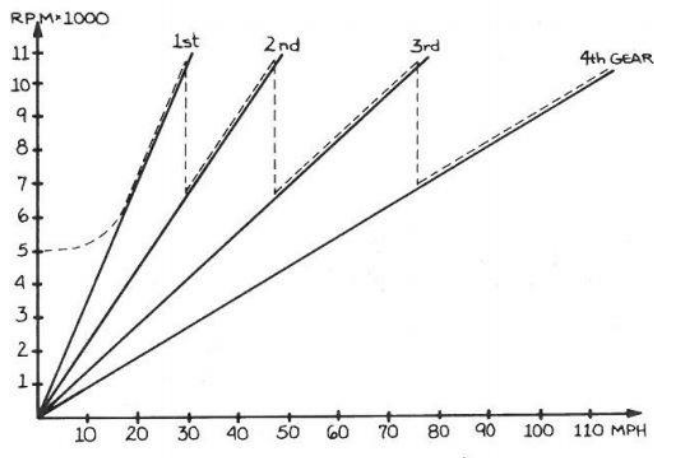
\includegraphics[width=\textwidth]{./illustrations/overview/discrete_transmission_shift_curve.png}
\end{minipage}
\hfill
\begin{minipage}{0.48\textwidth}
    \centering
    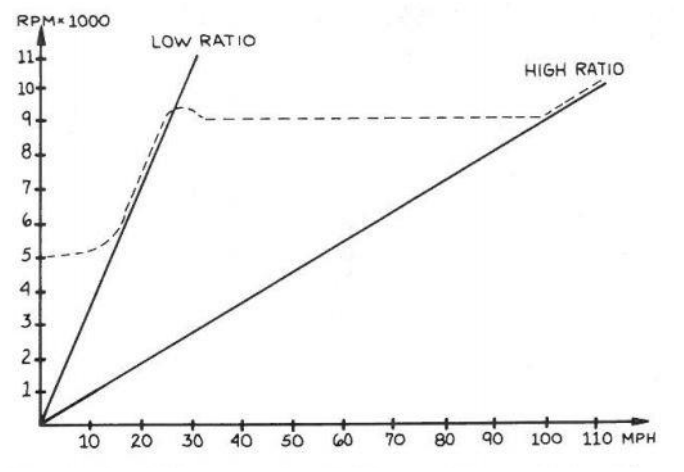
\includegraphics[width=\textwidth]{./illustrations/overview/cvt_shift_curve.png}
\end{minipage}
\caption{Illustrative comparison of engine speed versus vehicle speed. 
Left: stepped transmission showing discrete shifts. 
Right: continuously variable transmission showing smooth ratio evolution.}
\label{fig:cvt_vs_gearbox}
\end{figure}

% --------------------------------------------------------------
\subsection{Traction-Based Torque Transmission}

While the geometric adjustment of pulley radii determines the speed ratio, 
torque is transmitted through frictional interaction between the belt and 
the sheave faces.

When a pulley attempts to rotate, it applies a tangential force to the belt. 
For that force to be transmitted without relative motion, sufficient normal 
clamping force must press the belt against the conical surfaces. The greater 
the normal force, the greater the tangential force that can be supported 
before slip occurs.

This requirement arises directly from the nature of friction. The belt does 
not contain rigid gear teeth that mechanically lock the pulleys together. 
Instead, torque transfer depends on traction generated by contact pressure 
and surface friction. If the transmitted torque exceeds the available 
traction capacity, the belt will begin to slip relative to the sheave faces.

Slip reduces efficiency, generates heat, and can accelerate component wear. 
For this reason, CVT designs incorporate mechanisms that actively regulate 
clamping force in response to operating conditions.

It is therefore useful to distinguish between two interacting aspects of CVT behavior:
\begin{itemize}
    \item The \textbf{geometric ratio}, which determines relative speeds,
    \item The \textbf{traction capacity}, which determines how much torque can be transmitted without slip.
\end{itemize}

Both must be considered to fully understand performance.

\begin{figure}[H]
\centering
\begin{minipage}{0.48\textwidth}
    \centering
    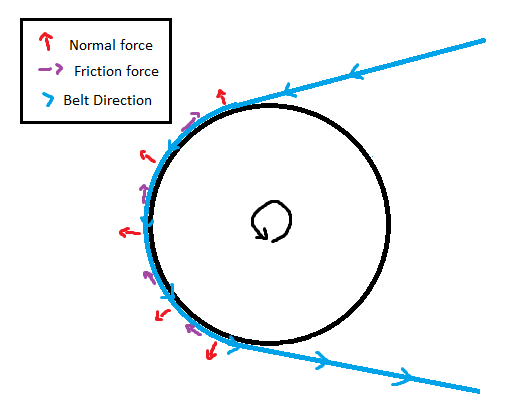
\includegraphics[width=\textwidth]{./illustrations/overview/single_pulley_normal_and_friction.png}
\end{minipage}
\hfill
\begin{minipage}{0.48\textwidth}
    \centering
    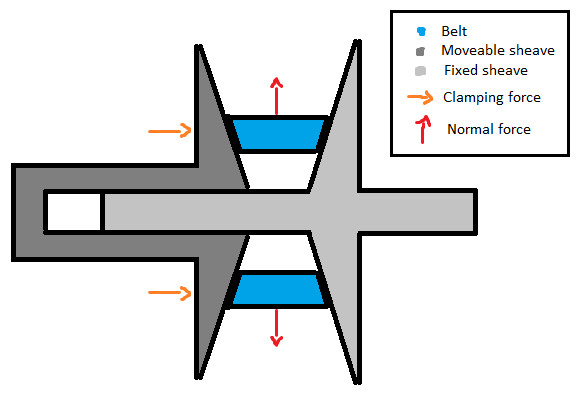
\includegraphics[width=\textwidth]{./illustrations/overview/cvt_cross_section_two_sheaves.png}
\end{minipage}
\caption{Belt-pulley contact mechanics and force transmission. 
Left: belt wrapped around a pulley showing normal forces (pressing belt against sheave surface) 
and tangential friction forces (transmitting torque through traction). 
Right: cross-sectional view of a CVT pulley assembly showing how axial clamping force 
between opposing sheaves generates the normal force required for friction and torque transmission.}
\label{fig:belt_contact}
\end{figure}

% --------------------------------------------------------------
\subsection{Actuation Mechanisms in the Present CVT}

While the geometric principles described above apply to all belt-type CVTs, 
the manner in which axial motion and clamping forces are generated depends 
on the specific hardware implementation.

The CVT considered in this work employs:

\begin{itemize}
    \item A \textbf{centrifugal flyweight and ramp mechanism} on the primary pulley,
    \item A \textbf{torque-feedback helix mechanism} on the secondary pulley,
    \item Compression and torsional springs that regulate axial clamping forces.
\end{itemize}

On the primary side, rotating flyweights move outward under centrifugal effects. 
Through a ramped interface, this outward motion generates axial force, which 
adjusts the sheave separation and alters the effective radius.


\begin{figure}[H]
\centering
\begin{minipage}{0.48\textwidth}
    \centering
    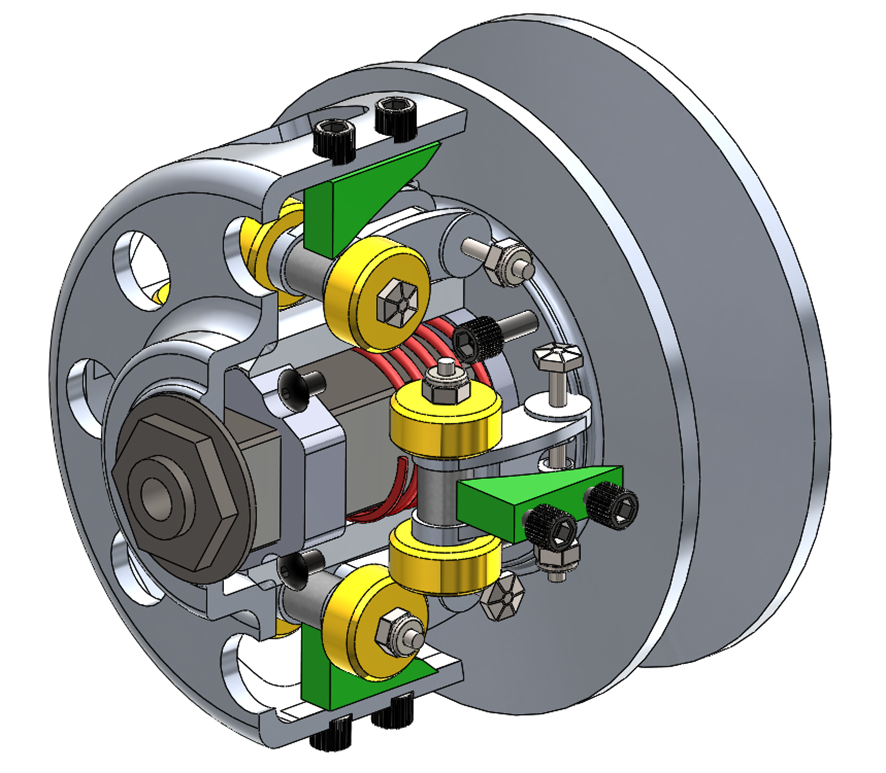
\includegraphics[width=\textwidth]{./illustrations/overview/primary_cvt_cad.png}
\end{minipage}
\hfill
\begin{minipage}{0.48\textwidth}
    \centering
    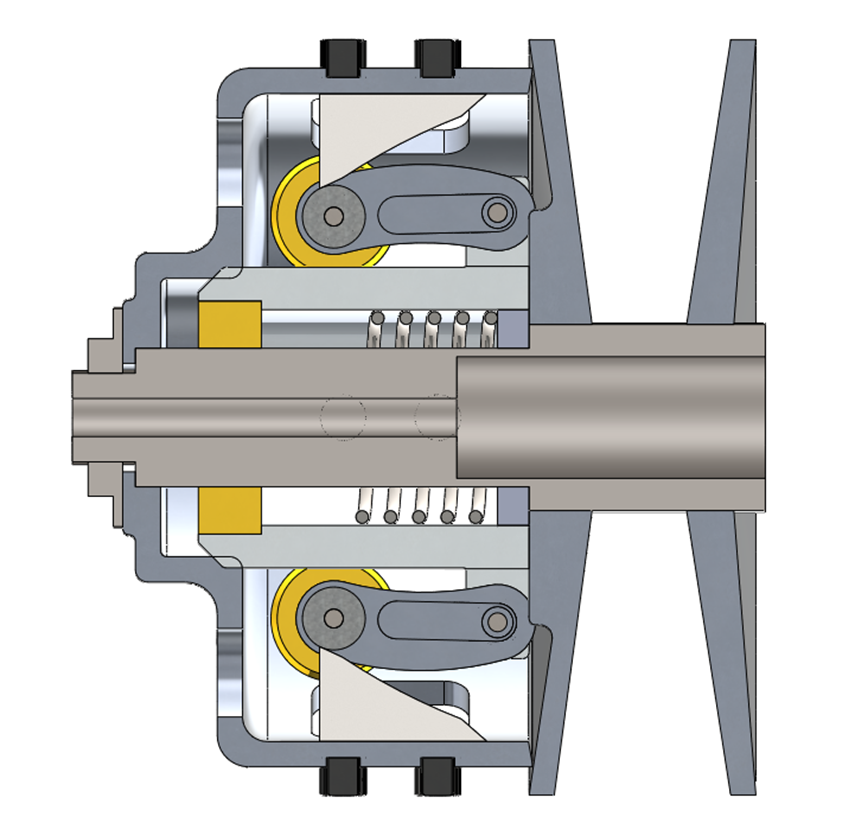
\includegraphics[width=\textwidth]{./illustrations/overview/primary_cvt_cad_cross_section.png}
\end{minipage}
\caption{Primary CVT pulley assembly. 
Left: exterior view. 
Right: cross-sectional view showing centrifugal flyweights (yellow), 
ramps (green), and compression spring (red). 
As engine speed increases, centrifugal force drives the flyweights outward along the ramps, 
generating axial clamping force.}
\label{fig:cvt_primary}
\end{figure}

On the secondary side, transmitted torque produces a rotational reaction within 
a helical interface. This interaction generates axial force that increases 
clamping in response to torque demand. Springs supplement this mechanism 
to regulate baseline clamping and system stability.

\begin{figure}[H]
\centering
\begin{minipage}{0.48\textwidth}
    \centering
    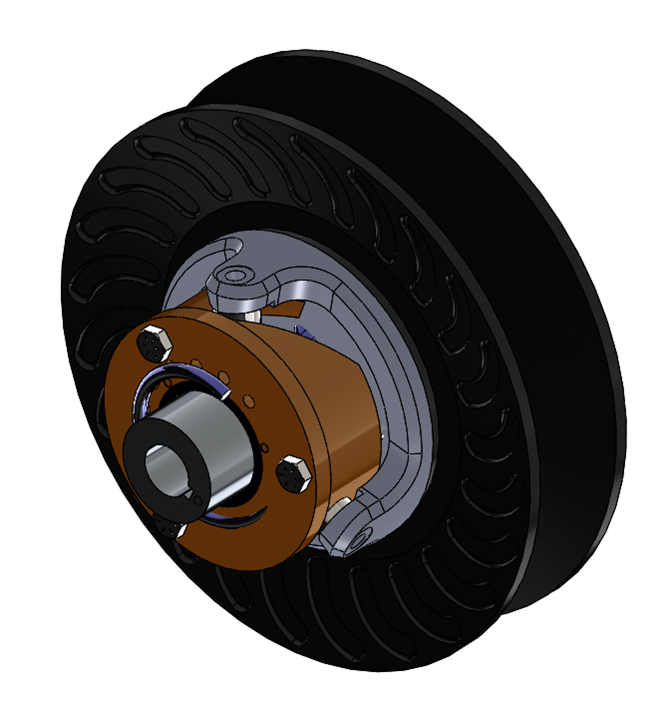
\includegraphics[width=\textwidth]{./illustrations/overview/secondary_cvt_cad.png}
\end{minipage}
\hfill
\begin{minipage}{0.48\textwidth}
    \centering
    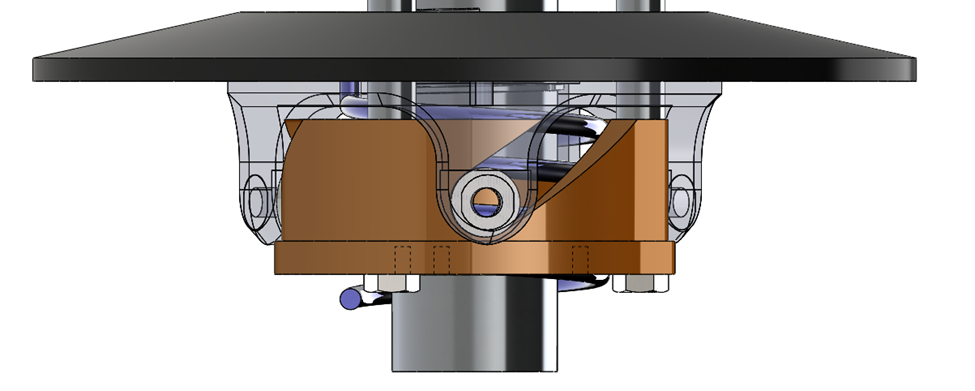
\includegraphics[width=\textwidth]{./illustrations/overview/secondary_cvt_cad_cross_section.png}
\end{minipage}
\caption{Secondary CVT pulley assembly. 
Left: exterior view. 
Right: cross-sectional view showing torque-feedback helix mechanism (bronze) 
and torsional spring (black). 
Transmitted torque generates a rotational reaction in the helix, 
which produces axial clamping force proportional to load.}
\label{fig:cvt_secondary}
\end{figure}

Although these mechanisms are specific to the hardware used in this system, 
the underlying principles of variable effective radius and traction-based 
torque transmission remain common to belt-driven CVTs.




% --------------------------------------------------------------
\subsection{Full Drivetrain Architecture}

The CVT does not operate in isolation. In the system considered here, 
the drivetrain consists of:

\begin{itemize}
    \item An internal combustion engine,
    \item The primary CVT pulley,
    \item A belt connecting to the secondary CVT pulley,
    \item A fixed-ratio gearbox,
    \item Final drive components and driven wheels,
    \item Tire-ground interaction generating tractive forces.
\end{itemize}

Engine torque enters the primary pulley, is transmitted through the belt 
to the secondary pulley, passes through a constant gear reduction, and 
ultimately produces tractive force at the ground.

The interaction between engine dynamics, CVT ratio evolution, drivetrain 
inertia, and external load forces governs overall vehicle performance.

\begin{figure}[H]
\centering

\includegraphics[width=0.5\textwidth]{./illustrations/overview/drivetrain_overview.png}
\caption{Overview of the complete drivetrain architecture considered in this work.}
\label{fig:drivetrain_overview}
\end{figure}


\section{Reference Material}\label{sec:notation}
This section records any information for easy reference.

\subsection{Coordinate and Sign Conventions}\label{sec:sign}

A consistent set of coordinate directions and sign conventions
is adopted throughout this document. All equations follow these conventions.

% --------------------------------------------------------------
\subsubsection{Vehicle Longitudinal Coordinate and Incline Angle}
\label{sec:vehicle_longitudinal}

Vehicle motion is modeled along a single longitudinal coordinate
that follows the surface of the road.

The coordinate $x$ is defined locally along the direction of travel,
tangent to the road surface. The positive direction, $+x$, corresponds
to the forward direction of vehicle motion.

Because the road may be inclined relative to horizontal, the local
direction of the $x$ axis depends on the road slope. The incline angle
is denoted by $\alpha$ and is measured between the road surface and a
horizontal reference line.

\[
\alpha > 0 \quad \text{: uphill in the $+x$ direction}
\]

\[
\alpha < 0 \quad \text{: downhill in the $+x$ direction}
\]

As illustrated in \Fig{fig:vehicle_longitudinal_axis}, the $x$ direction
always lies tangent to the road surface. Consequently, the orientation
of the longitudinal axis varies with the local road incline $\alpha$.

Vehicle velocity is defined along this coordinate. A velocity
$v > 0$ corresponds to motion in the forward $+x$ direction along
the road, while $v < 0$ corresponds to motion in the opposite direction.

These definitions establish the geometric orientation of vehicle motion
and the sign convention for road incline used throughout the model.

\begin{figure}[H]
\centering

\includegraphics[width=0.85\textwidth]{illustrations/coordinate/vehicle_longitudinal.png}
\caption{
Definition of the longitudinal vehicle coordinate and incline angle.
The coordinate $x$ is defined tangent to the road surface and
points in the forward direction of travel. The road incline
$\alpha$ is measured relative to the horizontal reference line.
Positive $\alpha$ corresponds to uphill motion in the $+x$
direction, while negative $\alpha$ corresponds to downhill slope.
}
\label{fig:vehicle_longitudinal_axis}
\end{figure}

% --------------------------------------------------------------
\subsubsection{Rotational Sign Convention}
\label{sec:rotational_sign}

All rotating components in the drivetrain follow a consistent angular
sign convention defined relative to forward vehicle motion.

The positive longitudinal direction $+x$ was defined previously as the
forward direction of travel along the road surface. The rotational
directions of all drivetrain components are chosen such that positive
rotation produces vehicle motion in this $+x$ direction.

As illustrated in \Fig{fig:rotational_sign}, positive wheel angular
velocity $\omega_w > 0$ corresponds to wheel rotation that drives the
vehicle forward along $+x$.

The same convention is propagated upstream through the drivetrain.
Positive rotation of the secondary pulley, $\omega_s > 0$, corresponds
to the direction of rotation that produces this forward wheel motion
through the final reduction gearbox and axle.

Likewise, positive rotation of the primary pulley, $\omega_p > 0$,
corresponds to the direction that drives the secondary pulley in this
same sense through the CVT belt.

Engine angular velocity follows the same convention. The engine rotates
positively when it drives the primary pulley in the defined positive
direction.

Torque follows the same sign convention. A torque is considered
positive when it acts in the defined positive rotational direction
and therefore tends to increase the corresponding angular velocity.

\begin{figure}[H]
\centering

\includegraphics[width=0.9\textwidth]{./illustrations/coordinate/rotational_directions.png}
\caption{
Rotational sign convention for the drivetrain. Positive angular
velocities for the wheels ($\omega_w$), secondary pulley ($\omega_s$),
and primary pulley ($\omega_p$) are defined such that drivetrain
rotation produces forward vehicle motion along the $+x$ direction.
}
\label{fig:rotational_sign}
\end{figure}

% --------------------------------------------------------------
\subsubsection{CVT Axial Direction}
\label{sec:cvt_axial_direction}

The axial coordinate of the primary pulley is defined along the axis of the
pulley shaft, parallel to the pulley centerline and perpendicular to the
plane of belt rotation.

In the reference configuration shown in
\Fig{fig:cvt_axial_direction} (left), the primary pulley is fully open.
The movable sheave is separated from the fixed sheave by the initial gap,
and this configuration defines the origin of the axial coordinate.

The axial variable $s$ measures the translation of the movable sheave
relative to this open configuration.

\[
s = 0 \quad \text{: fully open configuration}
\]

A positive value of $s$ corresponds to the movable sheave translating
toward the fixed sheave along the pulley axis.

\[
s > 0 \quad \text{: sheave closing motion}
\]

As the movable sheave closes, the belt is squeezed between the conical
faces and is forced outward along the pulley ramps. This increases the
effective belt radius on the primary pulley and corresponds to an
upshift of the transmission.

The maximum displacement $s = S_{\max}$ corresponds to the fully closed
configuration shown in \Fig{fig:cvt_axial_direction} (right).

Although $s$ is defined using the primary pulley, the motion cannot
occur independently. Because the belt length remains constrained,
closure of the primary pulley forces the secondary pulley to open.
The precise geometric relationship between these motions will be
derived later.

Axial velocity follows the same sign convention: $\dot{s} > 0$
corresponds to the movable sheave translating toward the fixed
sheave.

\begin{figure}[H]
\centering

\includegraphics[width=0.9\textwidth]{illustrations/coordinate/axial_direction.png}
\caption{
Definition of the primary axial coordinate. The system begins in an open 
configuration. The axial displacement $s$ measures how much the movable 
sheave has closed from this initial position. Increasing $s$ increases 
primary effective radius and is coupled to secondary axial motion.
}
\label{fig:cvt_axial_direction}
\end{figure}

% --------------------------------------------------------------
\subsubsection{Radial and Tangential Directions}
\label{sec:radial_direction}

Within the plane of pulley rotation, directions are defined using the
standard polar coordinate convention commonly used in rotational mechanics.

At any point in the plane, two orthogonal directions are defined:
the radial direction $\hat e_r$ and the tangential direction $\hat e_\theta$.
These directions form a local coordinate basis centered on the pulley axis.

The radial direction lies in the plane of rotation and points directly
outward from the center of the pulley. A radial force is defined as
positive when it acts away from the center of rotation. Thus,
$F_r > 0$ corresponds to a force directed outward along $\hat e_r$.

The tangential direction lies in the plane of rotation and is
perpendicular to the radial direction. The positive tangential
direction $\hat e_\theta$ is defined to be consistent with the
positive rotational convention introduced in
\Sec{sec:rotational_sign}. Tangential motion in this direction
corresponds to motion produced by positive angular velocity.

Figure~\ref{fig:radial_direction} illustrates these directions using
physical examples from the primary pulley. The centrifugal flyweights
generate outward radial forces $F_r$, while the belt moves along the
tangential direction with velocity $v_t$. These quantities serve as
representative examples of forces and motion that act along the radial
and tangential directions.

The previously defined axial direction is perpendicular to this plane
of rotation and points along the pulley shaft, into the page.

\begin{figure}[H]
\centering

\includegraphics[width=0.75\textwidth]{illustrations/coordinate/radial_tangential_direction.png}
\caption{
Radial and tangential directions in the plane of pulley rotation.
The radial direction $\hat e_r$ points outward from the center of the
pulley, while the tangential direction $\hat e_\theta$ is perpendicular
to $\hat e_r$ and aligned with positive rotation. Example quantities
illustrated include outward radial forces $F_r$ generated by flyweights
and tangential belt velocity $v_t$. For reference, the previously defined
axial coordinate $s$ is perpendicular to the page in this view and
points along the pulley shaft, into the page.
}
\label{fig:radial_direction}
\end{figure}


\subsection{Symbol Summary}\label{sec:symbols}
\begin{center}
\small
\setlength{\LTleft}{0pt}
\setlength{\LTright}{0pt}
\begin{longtable}{@{}p{0.34\textwidth}p{0.62\textwidth}@{}}
\toprule
Symbol & Meaning \\ \midrule
\endfirsthead
\toprule
Symbol & Meaning \\ \midrule
\endhead
\bottomrule
\endfoot
\bottomrule
\caption{Core symbols used throughout the derivation.}\label{tab:symbols_core}\\
\endlastfoot
\multicolumn{2}{@{}l}{\textbf{State and kinematics}} \\
$\vect{x}(t)$ & state vector \\
$t$ & time \\
$\omega_p,\ \omega_s$ & primary and secondary angular speed \\
$\alpha_p,\ \alpha_s$ & primary and secondary angular acceleration \\
$s,\ \dot s,\ \ddot s$ & shift position, velocity, and acceleration \\
$R,\ \dot R$ & CVT ratio and ratio rate \\
$v_{\mathrm{rel}}$ & relative slip speed at belt--pulley interface \\
\addlinespace
\multicolumn{2}{@{}l}{\textbf{Geometry}} \\
$r_{p,\mathrm{outer}}(s),\ r_{s,\mathrm{outer}}(s)$ & primary and secondary outer radius \\
$r_{p,\mathrm{eff}}(s),\ r_{s,\mathrm{eff}}(s)$ & primary and secondary effective torque radius \\
$r_{p,\text{outer},\min}$ & minimum primary outer radius \\
$r_{s,\text{outer},\max}$ & maximum secondary outer radius \\
$s_{\mathrm{dz}},\ s_{\max}$ & deadzone threshold and maximum shift \\
$\beta$ & sheave face half-angle (radial reference) \\
$C$ & pulley center distance \\
$L_b$ & total belt length \\
$\phi$ & belt wrap angle used in distributed contact model \\
$r,\ \dot r$ & local bConceptual Overview of Variable Geoelt path radius and its time derivative \\
$r_{\mathrm{cm}}$ & belt element center-of-mass radius \\
\addlinespace
\multicolumn{2}{@{}l}{\textbf{Constraint and mapping functions}} \\
$f(r_p,r_s,C)$ & belt-length compatibility root function ($f=0$) \\
$\operatorname*{root}_{r_s}(\cdot)$ & numerical root solve for secondary radius \\
$r_f(s),\ \dfrac{dr_f}{ds}$ & primary flyweight radius map and gradient \\
$\theta_s(s),\ \dfrac{d\theta_s}{ds}$ & secondary helix angle map and gradient \\
\addlinespace
\multicolumn{2}{@{}l}{\textbf{Forces and torques}} \\
$F_{p,\mathrm{ax}},\ F_{s,\mathrm{ax}}$ & primary and secondary axial mechanism force \\
$F_{c,p},\ F_{c,s}$ & primary and secondary belt centrifugal axial contribution \\
$F_{\mathrm{ax}}$ & generic axial clamp force at one pulley contact \\
$\tau_{\mathrm{eng}},\ \tau_{\mathrm{load}}$ & engine input torque and reflected load torque \\
$\tau_p,\ \tau_s$ & coupling torque seen at primary and secondary \\
$\tau,\ \tau_c$ & generic interface torque and applied coupling/friction torque \\
$\tau_{\mathrm{ns}}$ & no-slip requested coupling torque \\
$\tau_{\max}$ & traction-limited torque capacity \\
\addlinespace
\multicolumn{2}{@{}l}{\textbf{Mass/inertia and material parameters}} \\
$I_p,\ I_s$ & primary and secondary rotational inertia \\
$m_f$ & effective flyweight mass \\
$m_{p,m},\ m_{s,m}$ & equivalent primary and secondary translating mechanism mass \\
$\rho_b$ & belt material density \\
$A_b$ & belt cross-sectional area \\
$\mu$ & belt--pulley traction coefficient \\
$k_p,\ x_{p,0}$ & primary spring stiffness and preload displacement \\
$k_{s,\theta},\ \theta_{s,0}$ & secondary torsional stiffness and preload angle \\
$k_{s,x},\ x_{s,0}$ & secondary axial stiffness and preload displacement \\
\end{longtable}
\normalsize
\end{center}

\subsection{Base Units}

All quantities in this document are expressed in SI units unless otherwise stated.

\begin{table}[H]
\centering
\begin{tabular}{@{}lll@{}}
\toprule
Quantity & Unit & Symbol \\ \midrule
Length & meter & \si{\meter} \\
Mass & kilogram & \si{\kilogram} \\
Time & second & \si{\second} \\
Plane angle & radian & \si{\radian} \\
\bottomrule
\end{tabular}
\caption{Base SI units used by the model variables and parameters.}
\label{tab:si_base}
\end{table}

\subsection{Common Derived Units}

\begin{table}[H]
\centering
\begin{tabular}{@{}lll@{}}
\toprule
Quantity & Unit & Symbol \\ \midrule
Velocity & meter per second & \si{\meter\per\second} \\
Acceleration & meter per second squared & \si{\meter\per\second\squared} \\
Angular velocity & radian per second & \si{\radian\per\second} \\
Angular acceleration & radian per second squared & \si{\radian\per\second\squared} \\
Area & square meter & \si{\meter\squared} \\
Volume & cubic meter & \si{\meter\cubed} \\
Density & kilogram per cubic meter & \si{\kilogram\per\meter\cubed} \\
Linear spring stiffness & newton per meter & \si{\newton\per\meter} \\
Torsional spring stiffness & newton meter per radian & \si{\newton\meter\per\radian} \\
Force & newton (\si{\kilogram\meter\per\second\squared}) & \si{\newton} \\
Torque & newton meter (\si{\kilogram\meter\squared\per\second\squared}) & \si{\newton\meter} \\
Moment of inertia & kilogram meter squared & \si{\kilogram\meter\squared} \\
Power & watt (\si{\kilogram\meter\squared\per\second\cubed}) & \si{\watt} \\
Dimensionless ratios/coefs. & unitless & 1 \\
\bottomrule
\end{tabular}
\caption{Derived units and unitless groups used throughout the CVT model.}
\label{tab:si_derived}
\end{table}

\subsection{Constants and Parameters}\label{sec:constants}

All non-varying model parameters are centralized below as the canonical reference.
Unless explicitly treated as inputs or state-dependent maps, symbols listed here are held constant during simulation.

\begin{center}
\small
\setlength{\LTleft}{0pt}
\setlength{\LTright}{0pt}
\begin{longtable}{@{}p{0.15\textwidth}p{0.20\textwidth}p{0.14\textwidth}p{0.13\textwidth}p{0.32\textwidth}@{}}
\toprule
Symbol & Name & Nominal value & Unit & Description \\ \midrule
\endfirsthead
\toprule
Symbol & Name & Nominal value & Unit & Description \\ \midrule
\endhead
\bottomrule
\endfoot
\bottomrule
\caption{Canonical non-varying parameters used by the CVT model equations.}
\label{tab:constants}\\
\endlastfoot
\multicolumn{5}{@{}l}{\textbf{Geometry and belt}} \\
$L_b$ & Belt length & -- & \si{\meter} & Fixed total belt length \\
$C$ & Center distance & -- & \si{\meter} & Primary--secondary shaft center distance (fixed after initialization) \\
$\beta$ & Sheave half-angle & -- & \si{\radian} & Cone half-angle used for radial/axial conversion \\
$h_b$ & Belt thickness & -- & \si{\meter} & Radial belt thickness \\
$b_{\mathrm{out}}$ & Belt outer width & -- & \si{\meter} & Belt width at outer face \\
$b_{\mathrm{in}}$ & Belt inner width & -- & \si{\meter} & Belt width at inner face \\
$A_b$ & Belt cross-sectional area & -- & \si{\meter\squared} & Trapezoid area from $h_b$, $b_{\mathrm{out}}$, $b_{\mathrm{in}}$ \\
$r_{p,\text{outer},\min}$ & Primary minimum outer radius & -- & \si{\meter} & Radius at fully open primary \\
$r_{s,\text{outer},\max}$ & Secondary maximum outer radius & -- & \si{\meter} & Radius at fully closed secondary \\
$s_{\mathrm{dz}}$ & Shift deadzone threshold & -- & \si{\meter} & Onset of effective radial motion \\
$s_{\max}$ & Maximum shift & -- & \si{\meter} & Physical upper travel bound \\
\addlinespace
\multicolumn{5}{@{}l}{\textbf{Primary/secondary actuation}} \\
$m_f$ & Flyweight mass & -- & \si{\kilogram} & Effective flyweight mass \\
$r_{f,0}$ & Initial flyweight radius & -- & \si{\meter} & Flyweight radius offset at $s=0$ \\
$k_p$ & Primary spring stiffness & -- & \si{\newton\per\meter} & Primary compression spring rate \\
$x_{p,0}$ & Primary spring preload & -- & \si{\meter} & Initial compression of primary spring \\
$k_{s,\theta}$ & Secondary torsional stiffness & -- & \si{\newton\meter\per\radian} & Torsional spring rate in helix assembly \\
$\theta_{s,0}$ & Secondary torsional preload & -- & \si{\radian} & Initial torsional deflection preload \\
$r_h$ & Helix reference radius & -- & \si{\meter} & Effective cylindrical radius in helix kinematics \\
$k_{s,x}$ & Secondary axial stiffness & -- & \si{\newton\per\meter} & Secondary axial compression spring rate \\
$x_{s,0}$ & Secondary axial preload & -- & \si{\meter} & Initial compression of secondary axial spring \\
\addlinespace
\multicolumn{5}{@{}l}{\textbf{Inertia and drivetrain}} \\
$I_{\mathrm{eng}}$ & Engine inertia & -- & \si{\kilogram\meter\squared} & Engine rotational inertia \\
$I_{\mathrm{prim}}$ & Primary pulley inertia & -- & \si{\kilogram\meter\squared} & Primary CVT pulley inertia \\
$I_p$ & Effective primary inertia & -- & \si{\kilogram\meter\squared} & $I_p = I_{\mathrm{eng}} + I_{\mathrm{prim}}$ \\
$I_{\mathrm{sec}}$ & Secondary pulley inertia & -- & \si{\kilogram\meter\squared} & Secondary CVT pulley inertia \\
$I_{\mathrm{gb}}$ & Gearbox inertia & -- & \si{\kilogram\meter\squared} & Gearbox/intermediate shaft inertia \\
$I_{\mathrm{wheel}}$ & Wheel inertia & -- & \si{\kilogram\meter\squared} & Wheel/hub inertia about wheel axis \\
$I_s$ & Effective secondary inertia & -- & \si{\kilogram\meter\squared} & Lumped secondary-side inertia about secondary axis \\
$G$ & Final drive ratio & -- & 1 & Fixed ratio defined by $\omega_s = G\,\omega_w$ \\
$m$ & Vehicle mass & -- & \si{\kilogram} & Total vehicle mass \\
$r_w$ & Wheel rolling radius & -- & \si{\meter} & Effective tire rolling radius \\
\addlinespace
\multicolumn{5}{@{}l}{\textbf{Contact and environment}} \\
$\rho_b$ & Belt density & -- & \si{\kilogram\per\meter\cubed} & Belt material density \\
$\mu$ & Belt--pulley friction coefficient & -- & 1 & Effective Coulomb traction coefficient \\
$C_{\mathrm{rr}}$ & Rolling resistance coefficient & -- & 1 & Tire-road rolling resistance coefficient \\
$C_d$ & Drag coefficient & -- & 1 & Aerodynamic drag coefficient \\
$A_f$ & Frontal area & -- & \si{\meter\squared} & Vehicle aerodynamic reference area \\
$\rho$ & Air density & -- & \si{\kilogram\per\meter\cubed} & Ambient air density used in drag model \\
$g$ & Gravitational acceleration & -- & \si{\meter\per\second\squared} & Gravity constant \\
\end{longtable}
\normalsize
\end{center}

\section{Modeling Assumptions}\label{sec:assumptions}

The following assumptions define the modeling scope and physical idealizations
used in the CVT dynamic formulation. These assumptions establish the limits
within which the derived equations remain valid.

% ======================================================
\subsection{Material and Structural Idealizations}

\begin{assumptionblock}{assump:material_constancy}{Constant Material Properties}
Material properties of structural components are treated as constant.
No temperature-dependent material variation is modeled.
Thermal effects are not solved as part of this system.
\end{assumptionblock}

\begin{assumptionblock}{assump:rigid_components}{Rigid Structural Components}
All structural components (pulleys, shafts, housing) are modeled as rigid bodies.
Elastic deformation under operational loading is neglected.
The belt is assumed axially rigid (no longitudinal stretch),
while still conforming geometrically around pulleys.
\end{assumptionblock}

\begin{assumptionblock}{assump:no_wear}{Negligible Wear and Surface Evolution}
Component wear, belt degradation, and pulley surface evolution
are neglected.
The model represents short-term operational behavior.
\end{assumptionblock}

% ======================================================
\subsection{Contact and Friction Modeling}

\begin{assumptionblock}{assump:ideal_friction}{Idealized Belt--Pulley Friction Law}
Belt traction is modeled using a simplified friction law
(e.g., Coulomb friction with a capstan formulation and
an explicit stick--slip transition rule).
Microscopic contact mechanics, rubber hysteresis,
lubrication films, and detailed Stribeck effects
are not explicitly modeled.
\end{assumptionblock}

\begin{assumptionblock}{assump:constant_friction}{Constant Effective Friction Coefficient}
The belt--pulley coefficient of friction is treated as constant.
It does not evolve with temperature, wear, or surface conditioning.
\end{assumptionblock}

\begin{assumptionblock}{assump:uniform_contact}{Uniform Contact Distribution}
Contact pressure and traction over the pulley wrap angle
are treated as effectively uniform or averaged.
Localized edge loading and non-uniform stress distributions are neglected.
\end{assumptionblock}

% ======================================================
\subsection{Geometric and Kinematic Idealizations}

\begin{assumptionblock}{assump:axis_alignment}{Perfect Axis Alignment}
Primary and secondary pulley axes are assumed perfectly aligned.
Misalignment, shaft eccentricity, and geometric runout are neglected.
\end{assumptionblock}

\begin{assumptionblock}{assump:constant_belt_length}{Constant Belt Length}
The belt length is treated as constant.
Longitudinal elasticity, transient stretch, permanent creep, and
progressive elongation are not modeled.
Effective pulley radii are determined solely from geometry
and belt-length constraints.
\end{assumptionblock}

\begin{assumptionblock}{assump:uniform_contact_radius}{Uniform Contact Radius Around Wrap}
At any given instant, the belt contacts each pulley at a single,
uniform effective radius throughout the entire wrap angle.
The contact radius is constant around the circumference of contact,
with no spiral or progressive radial variation along the wrap.
While the effective radius may evolve with axial shift position,
it remains spatially uniform at each time instant.
\end{assumptionblock}

% ======================================================
\subsection{Dynamic and Inertial Modeling}

\begin{assumptionblock}{assump:lumped_inertia}{Lumped Inertia Representation}
Rotational inertias of the engine, pulleys, drivetrain,
and wheels are represented as lumped equivalent inertias.
Distributed shaft flex and torsional compliance are neglected.
\end{assumptionblock}

\begin{assumptionblock}{assump:no_vibration}{Negligible Vibrational Effects}
High-frequency vibrational effects, structural resonances,
and drivetrain oscillations are neglected.
The model captures dominant rigid-body dynamics only.
\end{assumptionblock}

\begin{assumptionblock}{assump:no_parasitic_losses}{Negligible Parasitic Friction}
Frictional losses in non-critical components
(e.g., bearings, seals, auxiliary shafts)
are neglected.
Only friction directly relevant to belt traction
and CVT torque transfer is modeled.
\end{assumptionblock}

\begin{assumptionblock}{assump:ideal_cvt_power}{Ideal CVT Power Transmission}
Power transmission through the CVT is modeled as ideal
(i.e., no internal dissipation).
Although belt slip is explicitly modeled and affects
torque capacity and shift dynamics,
the associated power loss $P_{\text{loss}}$ is neglected.
\end{assumptionblock}

\begin{assumptionblock}{assump:single_slip_interface}{Single Active Slip Interface}
At any instant, the belt is assumed to either adhere to both pulleys
or slip at exactly one pulley contact.
Simultaneous slip at both pulley contacts is not modeled.

If operating conditions would otherwise cause both contacts to exceed
their traction limits, the model assumes an instantaneous transition
between single-slip states.
\end{assumptionblock}

% ======================================================
\subsection{Environmental and Operational Scope}

\begin{assumptionblock}{assump:gravity_internal}{Negligible Gravitational Influence on CVT Internals}
Gravitational forces acting on CVT internal components
are negligible relative to centrifugal and contact forces
at operating speeds.
\end{assumptionblock}

\begin{assumptionblock}{assump:full_throttle_model}{Full-Throttle Engine Model}
The engine is modeled using a prescribed full-throttle torque curve.
Load feedback modifies engine speed dynamically,
but part-throttle dynamics and throttle transients
are not explicitly modeled.
\end{assumptionblock}


\section{Governing Principles}\label{sec:principles}

% NOTE:
% Using the format:
% \theory{th:key}{Title}{<equation>}{<description>}{<source>}[<derivation>]
%
% Keep th: keys stable so references never break.

% -------------------------
% Mechanics (forces/torques)
% -------------------------

\theory
{th:newton-trans}
{Newton's Second Law (Translation)}
{\sum F = m a}
{
\begin{itemize}
  \item $\sum F$ is the net force (\si{\newton})
  \item $m$ is mass (\si{\kilogram})
  \item $a$ is acceleration (\si{\meter\per\second\squared})
\end{itemize}
}
{Classical mechanics (textbook / lecture notes).}
[
From the definition of acceleration and empirical laws of motion; used here as a governing relationship.
]

\theory
{th:newton-rot}
{Newton's Second Law (Rotation)}
{\sum \tau = I \alpha}
{
\begin{itemize}
  \item $\sum \tau$ is net torque (\si{\newton\meter})
  \item $I$ is moment of inertia (\si{\kilogram\meter\squared})
  \item $\alpha$ is angular acceleration (\si{\radian\per\second\squared})
\end{itemize}
}
{Classical rigid body dynamics (textbook / lecture notes).}
[
Standard rigid-body rotational dynamics relationship.
]

\theory
{th:torque_definition}
{Torque Definition}
{\tau = F r}
{
\begin{itemize}
  \item $\tau$ is torque (\si{\newton\meter})
  \item $F$ is tangential force (\si{\newton})
  \item $r$ is moment arm radius (\si{\meter})
\end{itemize}
}
{Classical mechanics (textbook / lecture notes).}
[
Defines torque as the product of tangential force and moment arm.
Equivalently, $F = \tau / r$ gives the tangential force from a known torque.
]

\theory
{th:kinetic_energy_trans}
{Kinetic Energy (Translational)}
{T = \frac{1}{2} m v^2}
{
\begin{itemize}
  \item $T$ is kinetic energy (\si{\joule})
  \item $m$ is mass (\si{\kilogram})
  \item $v$ is velocity (\si{\meter\per\second})
\end{itemize}
}
{Classical mechanics (textbook / lecture notes).}
[
Translational kinetic energy of a point mass or rigid body moving with velocity $v$.
]

\theory
{th:centrifugal_force}
{Centrifugal Force}
{F_c = m \omega^2 r}
{
\begin{itemize}
  \item $F_c$ is centrifugal force (\si{\newton})
  \item $m$ is mass (\si{\kilogram})
  \item $\omega$ is angular velocity (\si{\radian\per\second})
  \item $r$ is radius from the axis of rotation (\si{\meter})
\end{itemize}
}
{\citet{CentrifugalForceCalculator2024}.}
[
Derived from circular motion kinematics where $a_c = \omega^2 r$, then applying $F = ma$.
]

% -------------------------
% Springs / elasticity
% -------------------------

\theory
{th:hooke_linear}
{Hooke's Law (Compressional)}
{F = k \Delta x}
{
\begin{itemize}
  \item $F$ is force (\si{\newton})
  \item $k$ is spring constant (\si{\newton\per\meter})
  \item $\Delta x$ is displacement (\si{\meter})
\end{itemize}
}
{\citet{hookeslaw}.}
[
Linear spring constitutive relationship in the elastic regime.
]

\theory
{th:hooke_torsional}
{Hooke's Law (Torsional)}
{F = \frac{k \Delta \theta}{r}}
{
\begin{itemize}
  \item $F$ is force (\si{\newton})
  \item $k$ is torsional spring constant (\si{\newton\meter\per\radian})
  \item $\Delta \theta$ is angular deflection (\si{\radian})
  \item $r$ is torque arm radius (\si{\meter})
\end{itemize}
}
{\citet{SpringDesignFormulas}.}
[
Starting from $\tau = k\Delta\theta$ and $\tau = Fr$, then $F = \frac{k\Delta\theta}{r}$.
]

% -------------------------
% Powertrain relationships
% -------------------------

\theory
{th:engine_torque_power}
{Engine Torque from Power}
{\tau = \frac{P}{\omega}}
{
\begin{itemize}
  \item $\tau$ is torque (\si{\newton\meter})
  \item $P$ is power (\si{\watt})
  \item $\omega$ is angular velocity (\si{\radian\per\second})
\end{itemize}
}
{\citet{HorsepowerCalculation}.}
[
From the rotational power relationship $P=\tau\omega$.
]

\theory
{th:gearing_torque}
{Gearing (Torque Scaling)}
{\tau_{\text{out}} = \tau_{\text{in}} \, R_{\text{gear}}}
{
\begin{itemize}
  \item $\tau_{\text{out}}$ is output torque (\si{\newton\meter})
  \item $\tau_{\text{in}}$ is input torque (\si{\newton\meter})
  \item $R_{\text{gear}}$ is gear reduction ratio (unitless)
\end{itemize}
}
{\citet{GearRatioExplanation}.}
[
Ideal gear relationship assuming no losses; power balance implies inverse scaling of speed.
]

% -------------------------
% Friction / belt traction
% -------------------------

\theory
{th:coulomb_friction}
{Coulomb Friction}
{F_f = \mu_s F_n}
{
\begin{itemize}
  \item $F_f$ is friction force (\si{\newton})
  \item $\mu_s$ is coefficient of static friction (unitless)
  \item $F_n$ is normal force (\si{\newton})
\end{itemize}
}
{\citet{FrictionWikipedia}.}
[
Coulomb friction model for impending slip.
]

\theory
{th:capstan}
{Capstan Equation}
{T_1 = T_2 e^{\mu \theta}}
{
\begin{itemize}
  \item $T_1$ is tight-side belt tension (\si{\newton})
  \item $T_2$ is slack-side belt tension (\si{\newton})
  \item $\mu$ is belt--pulley friction coefficient (unitless)
  \item $\theta$ is wrap angle (\si{\radian})
\end{itemize}
}
{\citet{CapstanEquation2021}.}
[
Differential force balance on an infinitesimal belt element on a pulley yields $\frac{\dd T}{T}=\mu\,\dd\theta$, then integrate over wrap.
]



% -------------------------
% Fluids / aero (if used)
% -------------------------

\theory
{th:density}
{Density}
{\rho = \frac{m}{V}}
{
\begin{itemize}
  \item $\rho$ is density (\si{\kilogram\per\meter\cubed})
  \item $m$ is mass (\si{\kilogram})
  \item $V$ is volume (\si{\meter\cubed})
\end{itemize}
}
{\citet{BritannicaDensity}.}
[
Definition of density.
]

\theory
{th:air_resistance}
{Air Resistance (Quadratic Drag)}
{F_d = \frac{1}{2}\rho v^2 C_d A}
{
\begin{itemize}
  \item $F_d$ is drag force (\si{\newton})
  \item $\rho$ is fluid density (\si{\kilogram\per\meter\cubed})
  \item $v$ is object speed relative to fluid (\si{\meter\per\second})
  \item $C_d$ is drag coefficient (unitless)
  \item $A$ is reference area (\si{\meter\squared})
\end{itemize}
}
{\citet{AirResistanceFormula}.}
[
Standard empirical/derived quadratic drag model; applicable at moderate to high Reynolds number.
]

\theory
{th:rolling_resistance}
{Rolling Resistance}
{F_r = C_r N}
{
\begin{itemize}
  \item $F_r$ is rolling resistance force (\si{\newton})
  \item $C_r$ is coefficient of rolling resistance (unitless)
  \item $N$ is normal force (\si{\newton})
\end{itemize}
}
{\citet{RollingResistance}.}
[
Rolling resistance arises from deformation of contact surfaces (tire and road). For a vehicle on level ground, $N = mg$ where $m$ is vehicle mass and $g$ is gravitational acceleration.
]

\theory
{th:gravity_force}
{Gravitational Force}
{F_g = mg}
{
\begin{itemize}
  \item $F_g$ is gravitational force (\si{\newton})
  \item $m$ is mass (\si{\kilogram})
  \item $g$ is gravitational acceleration (\si{\meter\per\second\squared})
\end{itemize}
}
{\citet{NewtonGravity}.}
[
Near Earth's surface, $g \approx 9.81$ \si{\meter\per\second\squared}. On an incline with angle $\theta$, the component parallel to the surface is $F_g \sin\theta$.
]


% ==============================================================

\section{System State Definition}
\label{sec:state}

The dynamic behavior of the CVT system is described using a set of
\emph{state variables}. A state variable is a quantity whose future
evolution is determined by its current value and the governing
differential equations of the system.

In numerical simulation, state variables are the quantities that are
explicitly integrated forward in time. All other model quantities
— such as torque transfer, transmission ratio, belt forces, and
contact conditions — are computed algebraically from these states.

% --------------------------------------------------------------
\subsection{State Vector}

\bigeq{eq:state-vector}{State Vector}{
\vect{x}(t) =
\begin{bmatrix}
\omega_p \\
\omega_s \\
s \\
\dot{s} \\
\hat{v}_b
\end{bmatrix}
}

where:

\begin{itemize}
    \item $\omega_p$ is the angular speed of the primary pulley 
    (\si{\radian\per\second}),

    \item $\omega_s$ is the angular speed of the secondary pulley 
    (\si{\radian\per\second}),

    \item $s$ is the axial shift position of the primary sheave
    (\si{\meter}),

    \item $\dot{s}$ is the axial shift velocity 
    (\si{\meter\per\second}).

    \item $\hat{v}_b$ is the modeled belt transport speed
    (\si{\meter\per\second}).
\end{itemize}

% --------------------------------------------------------------
\subsection{Independent Dynamic Degrees of Freedom}

These five quantities represent the independent dynamic motions of the CVT system.

The primary pulley can rotate independently under engine input and belt interaction. 
Its angular speed $\omega_p$ therefore represents one rotational degree of freedom.

The secondary pulley also rotates and interacts with both the belt and the external 
drivetrain load. Its angular speed $\omega_s$ represents a second independent 
rotational degree of freedom.

In addition to rotation, the CVT includes axial motion of the primary sheave. 
This axial displacement $s$ determines the effective pulley geometry and therefore 
the transmission ratio. The axial motion is mechanically independent of pure rotation 
and must be modeled explicitly.

Because axial motion follows second-order dynamics, both the axial position $s$ 
and its rate $\dot{s}$ are required to fully describe its evolution.

Finally, the belt itself moves through the pulley system and carries power
between the two pulleys. The quantity $\hat{v}_b$ describes the transport
speed of the belt and is included as a state variable so that this belt motion
can be represented directly within the dynamic model.

Together, these variables capture the complete rotational and axial motion of the system. 
Removing any one of them would eliminate an independent dynamic degree of freedom 
from the model.

% --------------------------------------------------------------
\subsection{Time Integration Perspective}

During numerical simulation, the state vector is advanced forward in time.

At each timestep $\Delta t$:

\begin{itemize}
    \item The angular speeds $\omega_p$ and $\omega_s$ are updated according 
    to their angular accelerations.

    \item The axial position $s$ is updated using its current velocity $\dot{s}$.

    \item The axial velocity $\dot{s}$ is updated according to the axial acceleration.
    
    \item The modeled belt transport speed $\hat{v}_b$ is updated according
    to its governing evolution law.
\end{itemize}

The angular and axial accelerations are determined from the governing 
equations derived in subsequent sections. Once the state vector has been 
updated, all other quantities in the model are computed directly from the 
current values of $\omega_p$, $\omega_s$, $s$, $\dot{s}$, and $\hat{v}_b$.


\section{Pulley Geometry}\label{sec:geometry}

This section establishes the geometric relationships that govern how axial
shift modifies the effective pulley radii and therefore the transmission ratio.

The analysis presented here is purely kinematic. No force balances or
dynamic effects are considered. The goal is to describe how pulley
geometry alone determines belt position and ratio evolution.

The objective is to derive explicit expressions for:

\begin{itemize}
    \item Primary outer radius as a function of shift,
    \item Secondary outer radius as a function of shift,
    \item Center-to-center distance,
    \item CVT ratio and its rate of change.
\end{itemize}

\paragraph{Radius Definitions Used in This Section}
Because the belt has finite radial height, two geometric radii are used here:
the \emph{outer radius} (belt outer surface/contact geometry) and the
\emph{inner radius} (belt inner surface). Let $h_b$ denote the belt height
(belt radial thickness). Then,
\[
r_{\text{inner}} = r_{\text{outer}} - h_b,
\]
The effective torque radius used in torque and ratio relations is introduced
later in \Sec{sec:effective-radius-placeholder}.

% ==============================================================
\subsection{Conceptual Overview of Variable Geometry}

As introduced in \Sec{sec:cvt_overview}, each pulley consists of two opposing
conical sheaves. One sheave is fixed axially, while the other translates along
the shaft.

The key controllable motion in the system is this \textit{axial separation}
between the sheaves. When the movable sheave translates toward the fixed
sheave, the gap narrows and the belt is forced outward along the conical faces.
When the sheaves separate, the belt settles deeper between them.

This axial motion does not directly change the pulley radius. Instead, the
effective radius arises geometrically from where the belt sits within the
sheave gap. In other words, axial displacement determines the belt's radial
position, and therefore the effective pulley radius. The precise relationship
between these quantities will be derived in the following subsection.

Because the belt length remains constrained, the effective radii of the
primary and secondary pulleys cannot vary independently. An increase in the
primary effective radius must therefore be accompanied by a corresponding
decrease in the secondary effective radius. This geometric coupling is
fundamental to CVT operation and forms the basis of the ratio model derived
below.

\begin{figure}[H]
\centering
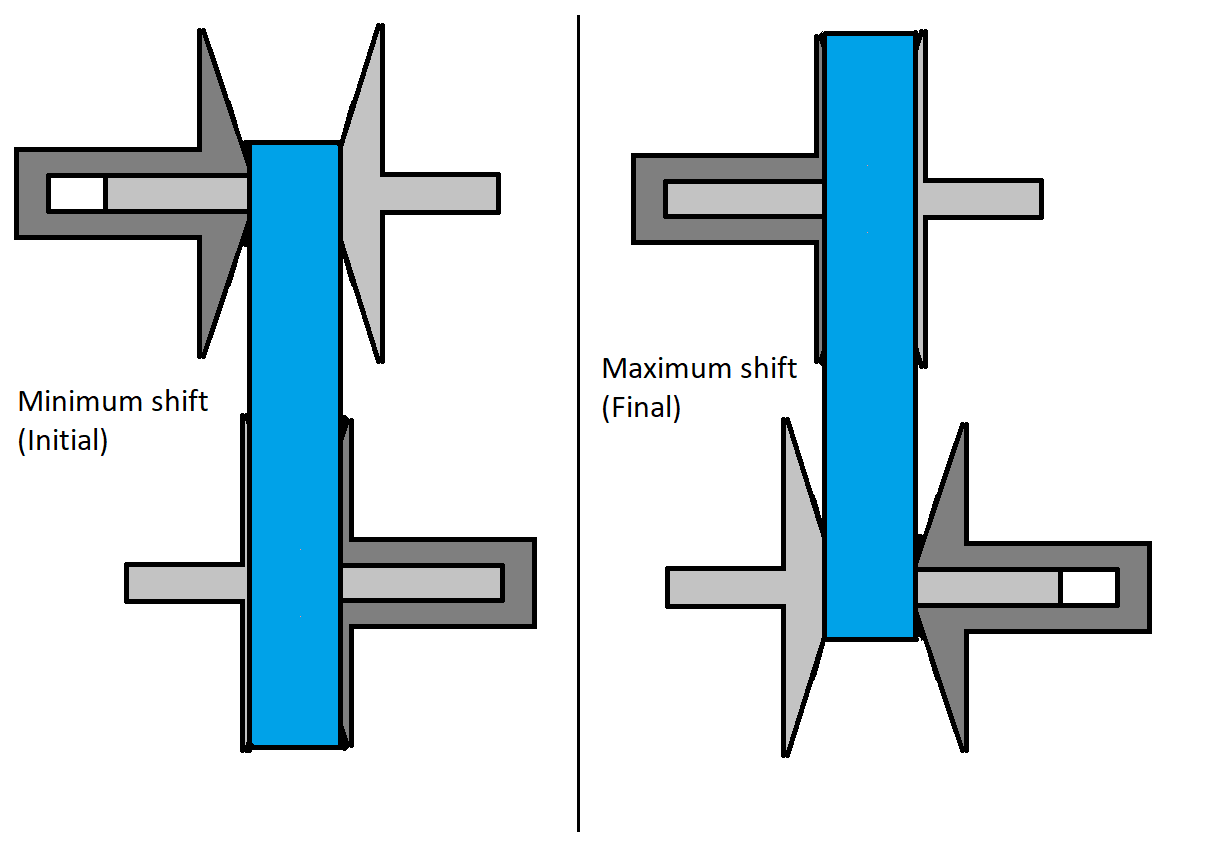
\includegraphics[width=0.95\textwidth]{illustrations/geometry/both_cvts_min_max_shift_belt.png}
\caption{
Conceptual illustration of variable pulley geometry.
Changes in axial separation alter effective radii.
Because belt length is constrained, an increase in primary effective
radius corresponds to a decrease in secondary effective radius.
}
\label{fig:variable_geometry}
\end{figure}

% NOTE:
% - Clarify cone geometry assumptions
% - Clarify belt thickness uniformity
% - Clarify that geometry is idealized

% ==============================================================
% --------------------------------------------------------------
% --------------------------------------------------------------
\subsection{Definition of Axial Shift Variable}
\label{sec:shift_definition}

Let $s$ denote the axial displacement of the movable primary sheave,
defined according to the sign convention in \Sec{sec:cvt_axial_direction}.

At $s = 0$, the primary pulley is in its fully open configuration.
The sheaves are at their maximum axial separation, and the belt
rests at its minimum effective radius.

The shift coordinate $s$ measures the amount of closure relative
to this initial configuration. Increasing $s$ corresponds to the
movable sheave translating toward the fixed sheave, reducing the
axial gap.

% --------------------------------------------------------------
\paragraph{Deadzone and Travel Limits}

In practice, the initial sheave gap at $s = 0$ is larger than the
belt width. As a result, small axial motion does not immediately
alter the belt’s contact position on the conical faces.

The interval
\[
0 \le s < s_{\mathrm{dz}}
\]
defines this \emph{deadzone}. Within this region, the movable
sheave translates axially but does not yet sufficiently compress
the belt to change its effective contact radius. The belt remains
at the same radial position despite the reduction in gap.

Once the sheave gap becomes small enough to fully engage the belt,
further axial motion alters the belt position. For
\[
s_{\mathrm{dz}} \le s \le s_{\max},
\]
additional closure forces the belt outward along the conical faces,
producing a proportional change in primary effective radius.

The shift coordinate is therefore bounded as
\[
0 \le s \le s_{\max}.
\]

The upper limit $s_{\max}$ corresponds to the physical travel limit
of the sheave assembly. At this position, the sheaves are fully closed
and mechanically contact one another, forming a hard geometric boundary
beyond which further axial motion is not possible.


% ==============================================================
\subsection{Primary Outer Radius as a Function of Shift}
\label{sec:rp}

When the primary sheaves close beyond the deadzone, the belt is forced
outward along the conical faces. The relationship between axial closure
and radial expansion follows directly from the cone geometry.

As shown in \cref{fig:primary_geometry}, the sheave face forms a straight
line in cross-section. The cone half-angle $\beta$ is defined as the angle
between the sheave face and the \emph{radial direction} (As defined in \Sec{sec:radial_direction}). 

For a small axial displacement $\Delta s$
beyond the deadzone, the total closure is shared symmetrically between
the two opposing sheaves, so each sheave contributes $\Delta s/2$.

From the right triangle formed by the sheave face,
\[
\tan\beta = \frac{\Delta s/2}{\Delta r},
\]
which gives
\begin{equation}
\Delta r = \frac{\Delta s}{2\tan\beta}.
\label{eq:cone_geometry}
\end{equation}

Thus, the cone angle determines how axial motion is converted into
radial growth: smaller $\beta$ produces greater radial change for the
same axial displacement.

Taking the infinitesimal limit of \cref{eq:cone_geometry} yields the
local geometric relationship between axial shift and effective radius,
\begin{equation}
\frac{dr}{ds} = \frac{1}{2\tan\beta}.
\label{eq:cone_geometry_diff}
\end{equation}

Because the sheave face is straight, this derivative is constant,
meaning that radial position varies linearly with axial displacement.

\begin{figure}[H]
\centering
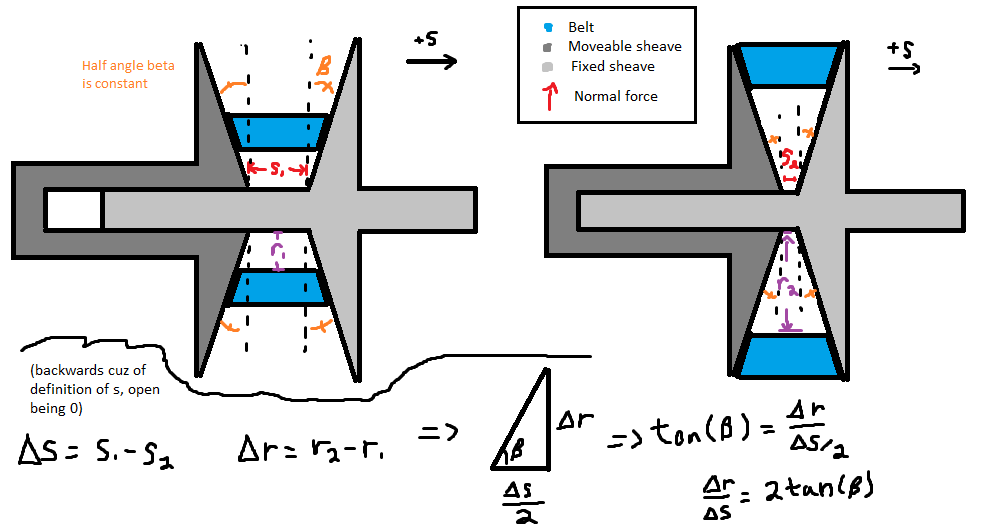
\includegraphics[width=0.7\linewidth]{./illustrations/geometry/primary_geometry.png}
\caption{
Axial–radial relationship for opposing conical sheaves.
The angle $\beta$ is defined between the sheave face and the radial direction.
}
\label{fig:primary_geometry}
\end{figure}

% --------------------------------------------------------------
\paragraph{Piecewise Radius Model}

Let $r_{p,\text{outer},\min}$ denote the minimum primary outer radius,
corresponding to the fully open configuration ($s=0$).

Within the deadzone, axial motion does not alter belt position.
Once $s \ge s_{\mathrm{dz}}$, only the displacement \emph{beyond the
deadzone} contributes to radial growth.

\bigeq{eq:primary_radius}{Primary Outer Radius}{
r_{p,\text{outer}}(s)=
\begin{cases}
r_{p,\text{outer},\min}, & 0 \le s < s_{\mathrm{dz}}, \\[8pt]
r_{p,\text{outer},\min} + \dfrac{s - s_{\mathrm{dz}}}{2\tan\beta},
& s_{\mathrm{dz}} \le s \le s_{\max}.
\end{cases}
}

% ============================================================== 
\subsection{Belt Length Constraint}\label{sec:belt_length}

In the previous subsection, the primary effective radius was expressed
as a function of axial shift. The secondary radius, however, cannot be
chosen independently. The belt has a fixed total length, and therefore
any change in primary radius must be accompanied by a corresponding
geometric adjustment of the secondary radius.

This section derives the geometric compatibility constraint imposed
by constant belt length. By expressing the total belt length in terms
of the primary radius $r_p$, secondary radius $r_s$, and center-to-center
distance $C$, we obtain an implicit relationship that couples the two
pulley radii.

The derivation follows directly from the belt path geometry shown in
\cref{fig:belt_geometry_placeholder}. The geometric
quantities used in the derivation are

\begin{itemize}
\item $r_p$ — radius of the primary pulley
\item $r_s$ — radius of the secondary pulley
\item $C$ — center-to-center distance between pulley shafts
\item $\phi_p$ — belt wrap angle on the primary pulley
\item $\phi_s$ — belt wrap angle on the secondary pulley
\item $\ell$ — length of a single straight tangent span
\end{itemize}


\begin{figure}[h]
\centering
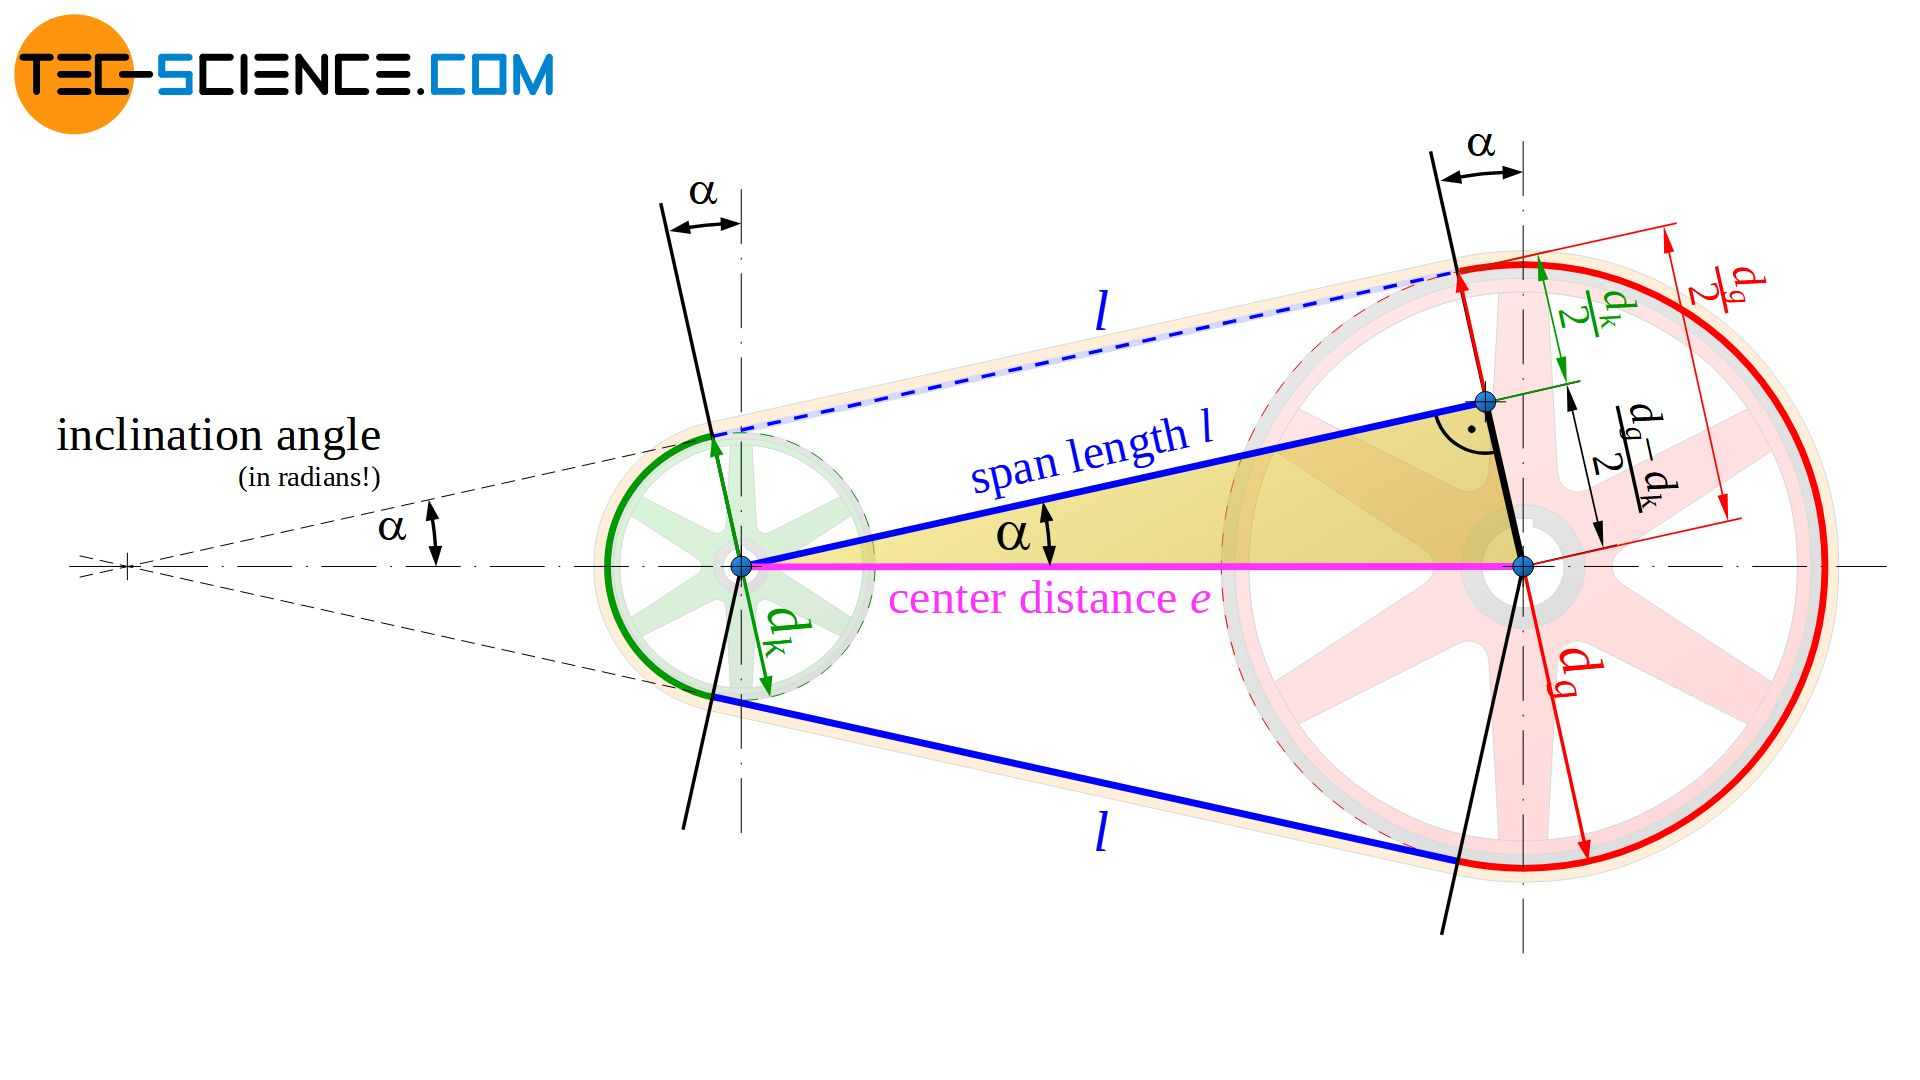
\includegraphics[width=0.75\linewidth]{./illustrations/belt_length_geometry.jpg}
\caption{Belt geometry for two pulleys of radii $r_p$ and $r_s$ separated by center distance $C$.
The belt wraps the pulleys with angles $\phi_p$ and $\phi_s$ and connects via two straight tangent spans $\ell$.}
\label{fig:belt_geometry_placeholder}
\end{figure}


\paragraph{Belt Length Decomposition}

The total belt length $L_b$ is the sum of:
(i) wrapped arc length on the primary pulley,
(ii) wrapped arc length on the secondary pulley, and
(iii) two straight tangent spans.
Therefore,

\begin{equation}
L_b = r_p \phi_p + r_s \phi_s + 2\ell,
\label{eq:belt_length_general}
\end{equation}

where $\ell$ is the length of a single straight tangent span segment.

\paragraph{Straight Span Length}

From the right-triangle geometry formed by the pulley centers and tangent points,

\begin{equation}
\ell = \sqrt{C^2 - (r_s - r_p)^2}.
\label{eq:span_length}
\end{equation}

\paragraph{Wrap Angles}

The wrap angles on the primary and secondary pulleys are

\begin{align}
\phi_p &= \pi - 2\lambda, \label{eq:wrap_primary}\\
\phi_s &= \pi + 2\lambda. \label{eq:wrap_secondary}
\end{align} 

If $\lambda < 0$, these expressions automatically redistribute wrap
between pulleys while preserving total belt length.

\paragraph{Tangency Angle (Signed Convention)}

Let $\lambda$ denote the signed angle between the line of centers and the straight
tangent belt segment (as defined in \Fig{fig:belt_geometry_placeholder}). We define

\begin{equation}
\sin\lambda = \frac{r_s - r_p}{C},
\label{eq:lambda_def}
\end{equation}

and equivalently,

\begin{equation}
\lambda = \sin^{-1}\!\left(\frac{r_s - r_p}{C}\right).
\label{eq:lambda_asin}
\end{equation}

Under this convention, $\lambda$ may be negative when $r_p > r_s$.
This signed definition ensures the wrap distribution automatically adjusts
when the pulley ordering reverses.

\paragraph{Closed Form Belt-Length Expression}

Substituting \Eq{eq:span_length} and \Eq{eq:wrap_primary}--\Eq{eq:wrap_secondary}
into \Eq{eq:belt_length_general} yields

\begin{align}
L_b
&= r_p(\pi - 2\lambda)
 + r_s(\pi + 2\lambda)
 + 2\sqrt{C^2 - (r_s - r_p)^2} \nonumber\\
&= \pi(r_p + r_s)
 + 2\lambda (r_s - r_p)
 + 2\sqrt{C^2 - (r_s - r_p)^2}. 
\label{eq:belt_length_subbed}
\end{align}

Finally, substituting \Eq{eq:lambda_asin} gives

\begin{equation}
L_b =
\pi(r_p + r_s)
+ 2(r_s - r_p)\,
\sin^{-1}\!\left(\frac{r_s - r_p}{C}\right)
+ 2\sqrt{C^2 - (r_s - r_p)^2}.
\label{eq:belt_length_final}
\end{equation}

\paragraph{Root Form (Geometric Compatibility Constraint)}

Rearranging \Eq{eq:belt_length_final} yields

\bigeq{eq:belt_length_root}{Belt Length Constraint Root Function}{
f(r_p, r_s, C) =
\pi(r_p + r_s)
+ 2(r_s - r_p)\,
\sin^{-1}\!\left(\frac{r_s - r_p}{C}\right)
+ 2\sqrt{C^2 - (r_s - r_p)^2}
- L_b.
}

The belt-length constraint is therefore

\begin{equation}
f(r_p, r_s, C) = 0.
\label{eq:belt_length_constraint}
\end{equation}

The form of \Eq{eq:belt_length_constraint} is unchanged if radii are defined
at the belt outer surface, inner surface, or effective mid-height radius,
provided all terms are referenced consistently. In particular, $L_b$ must
correspond to the same reference as $r_p$ and $r_s$ (e.g., outer-length with
outer radii, inner-length with inner radii, or effective-length with effective
radii).




\begin{remarkbox}[Remark (Transcendental Nature and Approximation)]

\Eq{eq:belt_length_root} is transcendental due to the
inverse-sine and square-root terms and therefore does not admit
a closed-form solution.

In this work, the constraint is solved numerically using a
bracketed root-finding method (e.g., bisection or Brent's method),
which is deterministic and robust over the physically admissible interval.

It is common in simplified treatments to assume

\[
\frac{r_s - r_p}{C} \approx 0,
\]

which implies $\lambda \approx 0$ and therefore
\[
\sin^{-1}\!\left(\frac{r_s - r_p}{C}\right) \approx 0.
\]

Under this small-angle assumption, the belt-length equation reduces to a much
simpler approximate form.

However, this approximation can introduce substantial geometric error when
$\frac{r_s - r_p}{C}$ is not small. Appendix~\ref{sec:approximation-validation}
quantifies this deviation and demonstrates that the approximation
is not acceptable under realistic operating conditions.

\end{remarkbox}


% NOTE:
% - Later sections will specify the bracketing bounds used in practice for the solver.
% - If you want to support cases where r_p > r_s, you can replace (r_s - r_p) with |r_s - r_p|
%   and state the sign convention, or explicitly assume w.l.o.g. r_s \ge r_p for the geometric derivation.



% ==============================================================
\subsection{Center-to-Center Distance Determination}\label{sec:center_distance}

In-order to make use of the belt-length constraint derived in \Sec{sec:belt_length}, 
the center-to-center distance $C$ must be determined.

The center-to-center distance $C$ is a fixed geometric parameter
of the assembled CVT system. Once the transmission is constructed,
$C$ does not vary during operation.

To determine $C$, we evaluate the belt-length constraint
\Eq{eq:belt_length_constraint} at the \emph{known} initial configuration
of the system.

\paragraph{Initial Geometric Configuration}

At startup, the CVT is assumed to be in its lowest ratio configuration:

\begin{itemize}
    \item The primary pulley is at its minimum outer radius,
    \[
    r_p = r_{p,\text{outer},\min}.
    \]
    \item The secondary pulley is at its maximum outer radius,
    \[
    r_s = r_{s,\text{outer},\max}.
    \]
\end{itemize}

These values are determined by the physical geometry of the sheaves
and represent the fully separated primary and fully closed secondary
configuration.

\paragraph{Center Distance from Belt-Length Compatibility}

Substituting these known radii into
\Eq{eq:belt_length_root} yields

\begin{equation}
f(r_{p,\text{outer},\min}, r_{s,\text{outer},\max}, C) = 0.
\label{eq:center_distance_constraint}
\end{equation}

This equation contains a single unknown, $C$, and is solved
numerically to determine the fixed center-to-center distance
consistent with the specified belt length $L_b$.

\begin{equation}
C
=
\operatorname*{root}_{C}
\; f\!\left(r_{p,\text{outer},\min}, r_{s,\text{outer},\max}, C\right).
\end{equation}

\begin{remarkbox}[Remark (One-Time Geometric Solve)]
The center distance $C$ is determined once during model
initialization. Thereafter, $C$ is treated as a constant
in all subsequent geometric and dynamic calculations.
\end{remarkbox}



% ==============================================================
\subsection{Secondary Outer Radius as a Function of Shift}
\label{sec:secondary_radius}

With the center-to-center distance $C$ determined from
\Sec{sec:center_distance}, and the primary radius
$r_{p,\text{outer}}(s)$ defined by \Eq{eq:primary_radius}, the secondary
outer radius is obtained by enforcing the belt-length
compatibility constraint.

\paragraph{Geometric Coupling}

At any shift position $s$, the primary radius
$r_{p,\text{outer}}(s)$ is known. The secondary radius $r_s$
must therefore satisfy

\begin{equation}
f\!\left(r_{p,\text{outer}}(s), r_s, C\right) = 0,
\label{eq:secondary_radius_constraint}
\end{equation}

where $f(\cdot)$ is defined in \Eq{eq:belt_length_root}.

\paragraph{Numerical Determination of $r_s(s)$}

Because \Eq{eq:secondary_radius_constraint} is transcendental
in $r_s$, the secondary radius is obtained numerically for
each value of $s$:

\bigeq{eq:secondary_radius}{Secondary Outer Radius}{
r_{s,\text{outer}}(s)
=
\operatorname*{root}_{r_s}
\; f\!\left(r_{p,\text{outer}}(s), r_s, C\right).
}

\begin{remarkbox}[Remark (Dynamic Root Solve)]
Unlike the center-distance calculation in
\Sec{sec:center_distance}, which is performed once during
initialization, this root solve is performed repeatedly
as the shift coordinate $s$ evolves during simulation.
Because the physically admissible interval for $r_s$ is bounded,
a bracketed solver (e.g., Brent’s method) converges rapidly.
\end{remarkbox}

With both $r_{p,\mathrm{outer}}(s)$ and $r_{s,\mathrm{outer}}(s)$ determined,
all geometric quantities describing the belt path can now be expressed
explicitly as functions of the shift coordinate $s$.

% ==============================================================
\subsection{Wrap Angles as Functions of Shift}\label{sec:wrap_angles}

The wrap angles on the primary and secondary pulleys
vary as the pulley radii change. Using the geometric relations from
\Sec{sec:belt_length}, the tangency angle becomes

\begin{equation}
\lambda(s)
=
\sin^{-1}\!\left(
\frac{
r_{s,\mathrm{outer}}(s)
-
r_{p,\mathrm{outer}}(s)
}{C}
\right).
\end{equation}

Substitution into the wrap-angle definitions yields

\begin{align}
\phi_p(s)
&=
\pi
-
2\sin^{-1}\!\left(
\frac{
r_{s,\mathrm{outer}}(s)
-
r_{p,\mathrm{outer}}(s)
}{C}
\right),\label{eq:wrap_angle_primary}\\[8pt]
\phi_s(s)
&=
\pi
+
2\sin^{-1}\!\left(
\frac{
r_{s,\mathrm{outer}}(s)
-
r_{p,\mathrm{outer}}(s)
}{C}
\right).\label{eq:wrap_angle_secondary}
\end{align}



% ==============================================================
\subsection{Effective Torque Radius}
\label{sec:effective-radius-placeholder}

All geometric relations derived thus far use the outer surface of the belt
as the reference radius. This simplifies the belt-length formulation and
pulley geometry.

Torque transmission, however, occurs through the belt cross-section.
The appropriate moment arm for torque is therefore located
approximately at the mid-height of the belt, as illustrated in 
\cref{fig:belt_cross_section_effective_radius}.

The effective torque radius for each pulley is defined as

\begin{equation}
r_{p,\text{eff}} = r_{p,\text{outer}} - \frac{h_b}{2},
\label{eq:primary_effective_radius}
\end{equation}

\begin{equation}
r_{s,\text{eff}} = r_{s,\text{outer}} - \frac{h_b}{2}.
\label{eq:secondary_effective_radius}
\end{equation}

\begin{figure}[H]
\centering
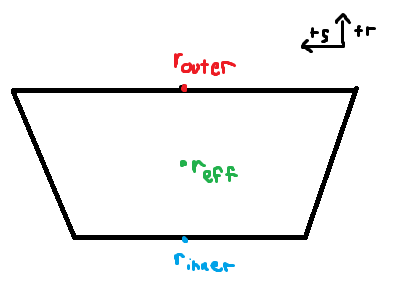
\includegraphics[width=0.6\linewidth]{./illustrations/geometry/belt_cross_section_effective_radius.png}
\caption{Belt cross-section showing the outer radius $r_{\text{outer}}$, 
inner radius $r_{\text{inner}}$, and effective torque radius $r_{\text{eff}}$ 
located at the belt mid-height. The effective radius is used for all torque 
and power transmission calculations.}
\label{fig:belt_cross_section_effective_radius}
\end{figure}


% ==============================================================
\subsection{CVT Ratio Definition}
\label{sec:cvt_ratio}

The instantaneous transmission ratio is determined purely by pulley geometry.
It is defined as the ratio of secondary to primary effective radii:

\bigeq{eq:cvt_ratio}{CVT Ratio}{
R(s) = \frac{r_{s,\text{eff}}(s)}{r_{p,\text{eff}}(s)}.
}

Because both effective radii are functions of the shift coordinate $s$,
the transmission ratio is likewise a function of $s$ alone.

As the primary sheaves close, $r_{p,\text{eff}}(s)$ increases.
By belt-length compatibility, the secondary radius decreases.
Consequently, the ratio $R(s)$ decreases with increasing $s$.

Thus:
\begin{itemize}
    \item Small $s$ (minimum primary radius) corresponds to high ratio.
    \item Large $s$ (maximum primary radius) corresponds to low ratio.
\end{itemize}

The CVT ratio is therefore a purely geometric quantity determined by
the axial shift position.


% ==============================================================
\subsection{Ratio Rate of Change}\label{sec:ratio_rate}

The CVT ratio is not only a function of shift position, but also changes in time whenever the
sheaves are moving. This time variation matters because a changing ratio introduces additional
kinematic coupling between the primary and secondary rotations. In other words, it is not
sufficient to know the instantaneous ratio $R(s)$; the model also requires how quickly the ratio
is changing.

This section derives an explicit expression for $\dot R$ in terms of the shift velocity $\dot s$
and geometric derivatives.

\subsubsection{Start from the Ratio Definition}

The ratio is defined by the effective radii as

\begin{equation}
R(s) = \frac{r_{s,\text{eff}}(s)}{r_{p,\text{eff}}(s)}.
\label{eq:R_def}
\end{equation}

Because $R$ depends on time only through $s(t)$, the chain rule gives

\begin{equation}
\dot R = \frac{dR}{ds}\dot s.
\label{eq:Rdot_chain}
\end{equation}

Thus, the objective is to compute $dR/ds$.

\subsubsection{Differentiate $R$ with Respect to $s$}

Differentiating \Eq{eq:R_def} with respect to $s$ (quotient rule) gives

\begin{align}
\frac{dR}{ds}
&=
\frac{d}{ds}\!\left(\frac{r_{s,\text{eff}}}{r_{p,\text{eff}}}\right)
=
\frac{
\left(\dfrac{dr_{s,\text{eff}}}{ds}\right) r_{p,\text{eff}}
-
r_{s,\text{eff}}
\left(\dfrac{dr_{p,\text{eff}}}{ds}\right)
}{
r_{p,\text{eff}}^2
}.
\label{eq:dRds_quotient}
\end{align}

Rearranging into a form that exposes the required components:

\begin{equation}
\frac{dR}{ds}
=
\frac{1}{r_{p,\text{eff}}}\frac{dr_{s,\text{eff}}}{ds}
-
\frac{r_{s,\text{eff}}}{r_{p,\text{eff}}^2}\frac{dr_{p,\text{eff}}}{ds}.
\label{eq:dRds_components}
\end{equation}


At this point, the remaining task is to express the two derivatives
$dr_{p,\text{eff}}/ds$ and $dr_{s,\text{eff}}/ds$ in computable form.

% ==============================================================
\subsubsection{Primary Radius Derivative}
\label{sec:drpds}

The primary radius derivative follows directly from the sheave geometry,
since the primary radius is prescribed explicitly as a function of shift.
From the piecewise primary radius model \Eq{eq:primary_radius}, the primary outer radius
satisfies

\[
r_{p,\text{outer}}(s)=
\begin{cases}
r_{p,\text{outer},\min}, & 0 \le s < s_{\mathrm{dz}}, \\[8pt]
r_{p,\text{outer},\min} + \dfrac{s - s_{\mathrm{dz}}}{2\tan\beta},
& s_{\mathrm{dz}} \le s \le s_{\max}.
\end{cases}
\]

Differentiating with respect to $s$ gives

\bigeq{eq:drpds_piecewise}{Primary Radius Derivative}{
\frac{dr_p}{ds}
=
\frac{dr_{p,\text{outer}}}{ds}
=
\begin{cases}
0, & 0 \le s < s_{\mathrm{dz}},\\[8pt]
\dfrac{1}{2\tan\beta}, & s_{\mathrm{dz}} \le s \le s_{\max}.
\end{cases}
}

Because $r_{p,\text{eff}} = r_{p,\text{outer}} - h_b/2$ and $h_b$ is constant,
the same derivative applies:

\begin{equation}
\frac{dr_{p,\text{eff}}}{ds} = \frac{dr_p}{ds}.
\label{eq:drpeffds}
\end{equation}


\begin{remarkbox}[Remark (At the Travel Limit)]
If the model clamps $s$ at the physical limit $s_{\max}$, then $r_{p,\text{outer}}$
(and thus $r_{p,\text{eff}}$) is constant beyond this point and the derivative is zero
for $s>s_{\max}$. In this document we restrict to the admissible domain
$0\le s\le s_{\max}$.
\end{remarkbox}

% ==============================================================
% ==============================================================
% ==============================================================
\subsubsection{Secondary Radius Derivative}
\label{sec:drsds}

Unlike the primary radius, the secondary radius is not prescribed explicitly
as a function of shift. Instead, it is determined implicitly by the
belt-length compatibility condition derived in \Sec{sec:belt_length}. Thus,
the secondary radius derivative must be obtained by differentiating the
constraint itself.

The belt-length constraint is written as

\begin{equation}
f(r_p, r_s, C) = 0,
\label{eq:belt_constraint_general}
\end{equation}

where $f(\cdot)$ is defined in \Eq{eq:belt_length_root} and $C$ is constant.

Since both $r_p=r_p(s)$ and $r_s=r_s(s)$ depend on the shift coordinate $s$,
differentiating \Eq{eq:belt_constraint_general} with respect to $s$ gives,
by the multivariable chain rule,

\begin{equation}
\frac{\partial f}{\partial r_p}\frac{dr_p}{ds}
+
\frac{\partial f}{\partial r_s}\frac{dr_s}{ds}
= 0.
\label{eq:implicit_chain}
\end{equation}

Solving \Eq{eq:implicit_chain} for the secondary radius derivative yields

\begin{equation}
\frac{dr_s}{ds}
=
-
\frac{\dfrac{\partial f}{\partial r_p}}
{\dfrac{\partial f}{\partial r_s}}
\frac{dr_p}{ds}.
\label{eq:drsds_general}
\end{equation}

Because the effective secondary radius differs from the outer radius only by
the constant belt offset $h_b/2$, the same derivative applies to the effective
radius:

\begin{equation}
\frac{dr_{s,\mathrm{eff}}}{ds} = \frac{dr_s}{ds}.
\label{eq:drseffds}
\end{equation}

Equation \Eq{eq:drsds_general} shows that the secondary radial motion is not
independent, but is instead determined by the belt-length constraint and the
primary radial motion.

At this point, the remaining task is to evaluate the two belt-constraint
sensitivities
$\partial f/\partial r_p$ and $\partial f/\partial r_s$, which appear in
\Eq{eq:drsds_general}. The following subsections derive these quantities
explicitly for the belt-length function defined in \Eq{eq:belt_length_root}.

\subsubsection{Partial Derivatives of the Belt Constraint}
\label{sec:belt_partials}

Recall the belt-length constraint written in root form as
\begin{equation}
f(r_p,r_s,C)
=
\pi(r_p+r_s)
+2(r_s-r_p)\sin^{-1}\!\left(\frac{r_s-r_p}{C}\right)
+2\sqrt{C^2-(r_s-r_p)^2}
-L_b
=0.
\label{eq:f_def_again}
\end{equation}

We now compute the two partial derivatives required in
\Eq{eq:drsds_general}, differentiating term-by-term and applying the
product rule directly to the inverse-sine term.

% --------------------------------------------------------------
\paragraph{Product rule for the inverse-sine factor}

Consider the factor
\[
(r_s-r_p)\sin^{-1}\!\left(\frac{r_s-r_p}{C}\right).
\]

Differentiating with respect to $r_p$ (product rule) gives
\begin{equation}
\frac{\partial}{\partial r_p}
\left[
(r_s-r_p)\sin^{-1}\!\left(\frac{r_s-r_p}{C}\right)
\right]
=
\underbrace{\frac{\partial}{\partial r_p}(r_s-r_p)}_{(1)}
\sin^{-1}\!\left(\frac{r_s-r_p}{C}\right)
+
(r_s-r_p)
\underbrace{\frac{\partial}{\partial r_p}\sin^{-1}\!\left(\frac{r_s-r_p}{C}\right)}_{(2)}.
\label{eq:prod_rule_asin_rp}
\end{equation}

We therefore compute the two sub-derivatives.

\subparagraph{Derivative (1)}

\begin{equation}
\frac{\partial}{\partial r_p}(r_s-r_p) = -1.
\label{eq:dlinear_rp}
\end{equation}

\subparagraph{Derivative (2)}

Using the chain rule,
\[
\frac{d}{dx}\sin^{-1}(x)=\frac{1}{\sqrt{1-x^2}},
\]
let
\[
u=\frac{r_s-r_p}{C}.
\]
Then
\[
\frac{\partial u}{\partial r_p} = -\frac{1}{C}.
\]

Therefore,
\begin{equation}
\frac{\partial}{\partial r_p}\sin^{-1}\!\left(\frac{r_s-r_p}{C}\right)
=
\frac{1}{\sqrt{1-u^2}}\left(-\frac{1}{C}\right).
\label{eq:asin_chain_rp_step1}
\end{equation}

Now simplify the denominator:
\[
\sqrt{1-u^2}
=
\sqrt{1-\left(\frac{r_s-r_p}{C}\right)^2}
=
\frac{\sqrt{C^2-(r_s-r_p)^2}}{C}.
\]

Substituting into \Eq{eq:asin_chain_rp_step1} yields
\begin{equation}
\frac{\partial}{\partial r_p}\sin^{-1}\!\left(\frac{r_s-r_p}{C}\right)
=
-\frac{1}{\sqrt{C^2-(r_s-r_p)^2}}.
\label{eq:asin_chain_rp_final}
\end{equation}

\subparagraph{Substitute into the product rule}

Substituting \Eq{eq:dlinear_rp} and \Eq{eq:asin_chain_rp_final} into
\Eq{eq:prod_rule_asin_rp} gives
\begin{align}
\frac{\partial}{\partial r_p}
\left[
(r_s-r_p)\sin^{-1}\!\left(\frac{r_s-r_p}{C}\right)
\right]
&=
(-1)\sin^{-1}\!\left(\frac{r_s-r_p}{C}\right)
+
(r_s-r_p)\left(
-\frac{1}{\sqrt{C^2-(r_s-r_p)^2}}
\right)
\nonumber\\[6pt]
&=
-\sin^{-1}\!\left(\frac{r_s-r_p}{C}\right)
-
\frac{r_s-r_p}{\sqrt{C^2-(r_s-r_p)^2}}.
\label{eq:prod_asin_rp_final}
\end{align}

% --------------------------------------------------------------
\paragraph{Derivative of the square-root term}

For the straight-span contribution,
\[
2\sqrt{C^2-(r_s-r_p)^2},
\]
we apply the chain rule:

\begin{equation}
\frac{\partial}{\partial r_p}
\left[
2\sqrt{C^2-(r_s-r_p)^2}
\right]
=
\frac{2(r_s-r_p)}
{\sqrt{C^2-(r_s-r_p)^2}}.
\label{eq:sqrt_general_rp}
\end{equation}

% --------------------------------------------------------------
\paragraph{Assemble $\partial f/\partial r_p$}

Differentiating \Eq{eq:f_def_again} term-by-term gives

\begin{align}
\frac{\partial f}{\partial r_p}
&=
\pi
+
2\left(
-\sin^{-1}\!\left(\frac{r_s-r_p}{C}\right)
-
\frac{r_s-r_p}
{\sqrt{C^2-(r_s-r_p)^2}}
\right)
+
\frac{2(r_s-r_p)}
{\sqrt{C^2-(r_s-r_p)^2}}
\nonumber\\[6pt]
&=
\pi
-
2\sin^{-1}\!\left(\frac{r_s-r_p}{C}\right).
\label{eq:dfdrp_final}
\end{align}

The square-root contributions cancel exactly.

% --------------------------------------------------------------
\paragraph{Derivative with respect to $r_s$}

The same procedure yields

\begin{equation}
\frac{\partial}{\partial r_s}
\left[
(r_s-r_p)\sin^{-1}\!\left(\frac{r_s-r_p}{C}\right)
\right]
=
\sin^{-1}\!\left(\frac{r_s-r_p}{C}\right)
+
\frac{r_s-r_p}{\sqrt{C^2-(r_s-r_p)^2}},
\label{eq:prod_asin_rs}
\end{equation}

and

\begin{equation}
\frac{\partial}{\partial r_s}
\left[
2\sqrt{C^2-(r_s-r_p)^2}
\right]
=
-\frac{2(r_s-r_p)}
{\sqrt{C^2-(r_s-r_p)^2}}.
\label{eq:sqrt_general_rs}
\end{equation}

Assembling terms gives

\begin{align}
\frac{\partial f}{\partial r_s}
&=
\pi
+
2\left(
\sin^{-1}\!\left(\frac{r_s-r_p}{C}\right)
+
\frac{r_s-r_p}
{\sqrt{C^2-(r_s-r_p)^2}}
\right)
-
\frac{2(r_s-r_p)}
{\sqrt{C^2-(r_s-r_p)^2}}
\nonumber\\[6pt]
&=
\pi
+
2\sin^{-1}\!\left(\frac{r_s-r_p}{C}\right).
\label{eq:dfdrs_final}
\end{align}


% --------------------------------------------------------------
\paragraph{Summary of Belt Constraint Partial Derivatives}

From the derivations above, the partial derivatives of the belt-length
constraint \Eq{eq:f_def_again} are

\begin{equation}
\frac{\partial f}{\partial r_p}
=
\pi
-
2\sin^{-1}\!\left(\frac{r_s-r_p}{C}\right),
\label{eq:dfdrp_summary}
\end{equation}

\begin{equation}
\frac{\partial f}{\partial r_s}
=
\pi
+
2\sin^{-1}\!\left(\frac{r_s-r_p}{C}\right).
\label{eq:dfdrs_summary}
\end{equation}

These expressions are globally valid under the geometric definition
of $\lambda$ given in \Eq{eq:lambda_asin} and require no piecewise
case distinction.




% ==============================================================
% ==============================================================

% ==============================================================
\subsubsection{Final Expression for the Secondary Radius Derivative}
\label{sec:drsds_final}

Equation \Eq{eq:drsds_general} expresses the secondary radius derivative in
terms of the belt-constraint partial derivatives and the primary radius derivative:

\begin{equation}
\frac{dr_s}{ds}
=
-
\frac{\dfrac{\partial f}{\partial r_p}}
{\dfrac{\partial f}{\partial r_s}}
\frac{dr_p}{ds}.
\label{eq:drsds_recalled}
\end{equation}

From \Sec{sec:belt_partials}, the partial derivatives of the belt-length constraint
\Eq{eq:belt_length_root} are

\begin{equation}
\frac{\partial f}{\partial r_p}
=
\pi
-
2\sin^{-1}\!\left(\frac{r_s-r_p}{C}\right),
\label{eq:dfdrp_final_used}
\end{equation}

\begin{equation}
\frac{\partial f}{\partial r_s}
=
\pi
+
2\sin^{-1}\!\left(\frac{r_s-r_p}{C}\right).
\label{eq:dfdrs_final_used}
\end{equation}

Substituting \Eq{eq:dfdrp_final_used} and \Eq{eq:dfdrs_final_used} into
\Eq{eq:drsds_recalled} gives

\begin{equation}
\frac{dr_s}{ds}
=
-
\frac{
\pi - 2\sin^{-1}\!\left(\dfrac{r_s-r_p}{C}\right)
}{
\pi + 2\sin^{-1}\!\left(\dfrac{r_s-r_p}{C}\right)
}
\frac{dr_p}{ds}.
\label{eq:drsds_subbed}
\end{equation}

Finally, substituting the piecewise primary radius derivative
\Eq{eq:drpds_piecewise} yields

\bigeq{eq:drsds_final}{Secondary Radius Derivative}{
\frac{dr_s}{ds}
=
\begin{cases}
0,
& 0 \le s < s_{\mathrm{dz}}, \\[12pt]
\displaystyle
-\frac{1}{2\tan\beta}
\frac{
\pi - 2\sin^{-1}\!\left(\dfrac{r_s-r_p}{C}\right)
}{
\pi + 2\sin^{-1}\!\left(\dfrac{r_s-r_p}{C}\right)
},
& s_{\mathrm{dz}} \le s \le s_{\max}.
\end{cases}
}

Because $r_{s,\mathrm{eff}} = r_s - h_b/2$ with $h_b$ constant, the same
expression applies to the effective secondary radius derivative:

\begin{equation}
\frac{dr_{s,\mathrm{eff}}}{ds} = \frac{dr_s}{ds}.
\label{eq:drseffds_final}
\end{equation}

% ==============================================================
\subsubsection{Final Expression for \texorpdfstring{$dR/ds$}{dR/ds} and \texorpdfstring{$\dot R$}{Rdot}}
\label{sec:dRds_final}

From \Eq{eq:dRds_components}, the ratio derivative is

\begin{equation}
\frac{dR}{ds}
=
\frac{1}{r_{p,\mathrm{eff}}}\frac{dr_{s,\mathrm{eff}}}{ds}
-
\frac{r_{s,\mathrm{eff}}}{r_{p,\mathrm{eff}}^2}\frac{dr_{p,\mathrm{eff}}}{ds}.
\label{eq:dRds_recalled}
\end{equation}

Using \Eq{eq:drpeffds} and \Eq{eq:drseffds_final}, this becomes

\begin{equation}
\frac{dR}{ds}
=
\frac{1}{r_{p,\mathrm{eff}}}\frac{dr_s}{ds}
-
\frac{r_{s,\mathrm{eff}}}{r_{p,\mathrm{eff}}^2}\frac{dr_p}{ds}.
\label{eq:dRds_sub_radii}
\end{equation}

Substituting \Eq{eq:drsds_subbed} into \Eq{eq:dRds_sub_radii} gives

\begin{equation}
\frac{dR}{ds}
=
\left[
-
\frac{1}{r_{p,\mathrm{eff}}}
\frac{
\pi - 2\sin^{-1}\!\left(\dfrac{r_s-r_p}{C}\right)
}{
\pi + 2\sin^{-1}\!\left(\dfrac{r_s-r_p}{C}\right)
}
-
\frac{r_{s,\mathrm{eff}}}{r_{p,\mathrm{eff}}^2}
\right]
\frac{dr_p}{ds}.
\label{eq:dRds_subbed_all}
\end{equation}

Finally, substituting the piecewise primary derivative \Eq{eq:drpds_piecewise}
yields the fully expanded result

\begin{equation}
\frac{dR}{ds}
=
\begin{cases}
0,
& 0 \le s < s_{\mathrm{dz}}, \\[14pt]
\displaystyle
\frac{1}{2\tan\beta}
\left[
-
\frac{1}{r_{p,\mathrm{eff}}}
\frac{
\pi - 2\sin^{-1}\!\left(\dfrac{r_s-r_p}{C}\right)
}{
\pi + 2\sin^{-1}\!\left(\dfrac{r_s-r_p}{C}\right)
}
-
\frac{r_{s,\mathrm{eff}}}{r_{p,\mathrm{eff}}^2}
\right],
& s_{\mathrm{dz}} \le s \le s_{\max}.
\end{cases}
\label{eq:dRds_final}
\end{equation}

Using the chain rule \Eq{eq:Rdot_chain}, $\dot R = (dR/ds)\dot s$. Substituting
\Eq{eq:dRds_final} and rearranging gives

\bigeq{eq:Rdot_final}{Rate of Change of Transmission Ratio}{
\dot R
=
\begin{cases}
0,
& 0 \le s < s_{\mathrm{dz}}, \\[14pt]
\displaystyle
-\frac{\dot s}{2\tan\beta\,r_{p,\mathrm{eff}}}
\left[
\frac{
\pi - 2\sin^{-1}\!\left(\dfrac{r_s-r_p}{C}\right)
}{
\pi + 2\sin^{-1}\!\left(\dfrac{r_s-r_p}{C}\right)
}
+
\frac{r_{s,\mathrm{eff}}}{r_{p,\mathrm{eff}}}
\right],
& s_{\mathrm{dz}} \le s \le s_{\max}.
\end{cases}
}

\subsection{Section Summary and Forward Connection}
\label{sec:geometry_summary}

This section established the complete \emph{geometric foundation} of the CVT model.
The development was intentionally kinematic: the objective was to derive a closed,
computable mapping from axial shift to pulley geometry and transmission ratio, without
introducing force balance, slip behavior, or torque relations.

At a high level, the geometry defines the chain
\[
s(t)
\;\longrightarrow\;
r_{p,\text{eff}}(s),\; r_{s,\text{eff}}(s)
\;\longrightarrow\;
R(s)
\;\longrightarrow\;
\dot R(s,\dot s),
\]
with each intermediate relationship derived explicitly from pulley and belt geometry.

\paragraph{Key Results Established}

The following geometric components are now defined and ready for use in subsequent modeling:

\begin{enumerate}
    \item \textbf{Primary radius law.}  
    \Eq{eq:primary_radius} provides the piecewise relationship between axial shift $s$
    and primary outer radius, including deadzone behavior and cone-angle dependence.

    \item \textbf{Belt-length compatibility constraint.}  
    \Eq{eq:belt_length_constraint} enforces constant belt length and defines the implicit,
    nonlinear coupling between $r_p$, $r_s$, and the center distance $C$.

    \item \textbf{Center distance determination.}  
    \Sec{sec:center_distance} fixes the assembled center-to-center distance $C$ by evaluating
    the belt constraint at a known geometric configuration. This solve is performed once
    during initialization.

    \item \textbf{Secondary radius as a function of shift.}  
    \Sec{sec:secondary_radius} defines $r_s(s)$ implicitly by solving the belt constraint at
    each shift position, producing the required redistribution of belt radius between pulleys.

    \item \textbf{Wrap angles as functions of shift.}  
    \Sec{sec:wrap_angles} defines the wrap angles $\phi_p(s)$ and $\phi_s(s)$ follow directly from the tangency geometry and
    are available for later contact, work, and belt-distribution calculations.

    \item \textbf{Effective torque radii.}  
    \Sec{sec:effective-radius-placeholder} corrects outer radii to effective radii using belt
    thickness, ensuring subsequent torque relations use an appropriate moment arm.

    \item \textbf{Ratio and ratio rate.}  
    \Eq{eq:cvt_ratio} defines the geometric ratio $R(s)$, and \Sec{sec:ratio_rate} provides
    $\dfrac{dR}{ds}$ and $\dot R$ via \Eq{eq:dRds_final} and \Eq{eq:Rdot_final}, including the
    deadzone condition where $R$ is constant.
\end{enumerate}

\paragraph{Structural Role in the Full Model}

These results form the geometric backbone of the CVT simulation. All subsequent sections treat
the relationships derived here as fixed mappings. In particular, later torque and force models
will use $r_{p,\text{eff}}(s)$ and $r_{s,\text{eff}}(s)$ as inputs, and shifting kinematics will
use $R(s)$ and $\dot R(s,\dot s)$ to relate primary and secondary motion during ratio change.

Several key properties are now clear:
(i) the geometric coupling is inherently nonlinear (through the belt-length constraint),
(ii) the deadzone is explicitly represented,
and (iii) within the admissible travel range the mappings are differentiable and suitable for
continuous-time simulation.

\paragraph{Transition to Dynamics}

With the geometry fully specified, the next objective is to determine how the shift coordinate
evolves in time. Subsequent sections introduce axial force generation (from pulley mechanisms and
belt interaction) to determine $\dot s$ and $\ddot s$. Once $\dot s$ is known, the ratio-rate
expression \Eq{eq:Rdot_final} provides the corresponding ratio evolution and the required
kinematic coupling between rotating components during shifting.


\section{Pulley Axial Force Models}\label{sec:axial}

The geometric relations developed in the previous section define how
the transmission ratio varies with axial shift. What remains is to
determine \emph{why} the shift coordinate $s(t)$ changes in time.

Axial motion of the sheaves is driven by clamping forces generated
within the primary and secondary assemblies. On the primary side,
centrifugal flyweights and springs produce an inward axial force
that tends to close the sheaves and increase radius. On the secondary
side, torque reaction and spring preload generate an opposing axial
force.

The evolution of the shift coordinate is governed by the
net axial force acting on the movable sheave assembly.
Applying Newton's second law in the axial direction
(\theoryRef{th:newton-trans}) gives

\begin{equation}
m \, \ddot{s}
=
F_{p,\text{ax}} - F_{s,\text{ax}},
\label{eq:axial_newton_base}
\end{equation}

where $F_{p,\text{ax}}$ and $F_{s,\text{ax}}$ denote the axial forces
generated by the primary and secondary mechanisms, respectively,
and $m$ is the effective axial inertia of the moving
components.

The purpose of this section is to derive expressions for
$F_{p,\text{ax}}$ and $F_{s,\text{ax}}$ as functions of the current
system state. Once these force models are established, the shift
acceleration $\ddot s$ follows directly, completing the dynamic
description of axial motion.

\begin{figure}[H]
\centering
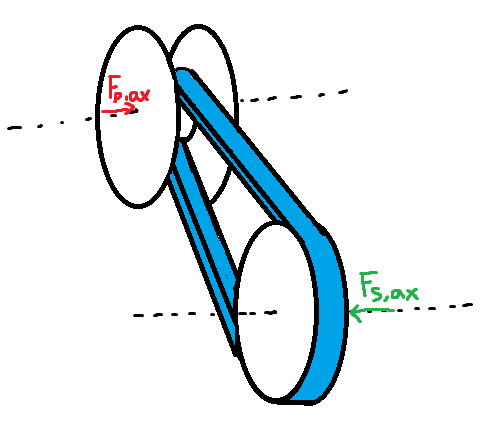
\includegraphics[width=0.8\textwidth]{illustrations/pulleyForces/cvt_overview_forces.png}
\caption{
Axial force balance governing sheave motion. Primary and secondary
mechanisms generate opposing axial forces. The net force determines
the shift acceleration $\ddot s$.
}
\label{fig:axial_force_balance}
\end{figure}

Although the specific actuator mechanisms modeled here correspond
to a flyweight-driven primary and a torque-reactive helix secondary,
the formulation is modular: any actuator model may be substituted
provided it returns the net axial force as a function of state.


% ==============================================================
\subsection{Ramp Geometry Parameterization}\label{sec:ramp-geometry}

Both pulley actuators redirect forces through inclined contact surfaces.
As the shift coordinate $s$ evolves, mechanical elements slide along
these surfaces, converting radial or circumferential forces into axial
clamping force.

To keep the formulation general and modular, the ramp geometries are
parameterized directly as functions of the axial shift coordinate $s$.
Any actuator profile may therefore be substituted provided it supplies
the appropriate geometric mapping and derivative.

% --------------------------------------------------------------
\paragraph{Primary Ramp Geometry (Axial-to-Radial Mapping)}

On the primary pulley, centrifugal force acting on the flyweights
is redirected into axial closing force through a ramp surface
(see \Fig{fig:primary_ramp}). As the movable sheave translates
axially, the flyweight slides along this ramp.

We represent the ramp by an axial-to-radial profile
\begin{equation}
r_f = r_f(s),
\label{eq:primary_profile}
\end{equation}
where $r_f(s)$ is the effective flyweight radius.

An incremental axial displacement $ds$ produces a radial displacement
$dr_f$. The local slope of the ramp is therefore $dr_f/ds$.
The instantaneous primary ramp angle is denoted by $\alpha_p(s)$ and is
defined with respect to the axial direction as
\begin{equation}
\tan\alpha_p(s) = \frac{dr_f}{ds},
\qquad
\alpha_p(s) = \tan^{-1}\!\left(\frac{dr_f}{ds}\right).
\label{eq:alpha_primary_from_slope}
\end{equation}

This definition follows directly from the geometry of the sliding
motion: a steeper ramp (larger $dr_f/ds$) produces greater radial
change per unit axial travel and therefore greater axial gain
when radial force is redirected through the surface.

\begin{figure}[H]
\centering
\begin{minipage}[t]{0.48\textwidth}
\centering
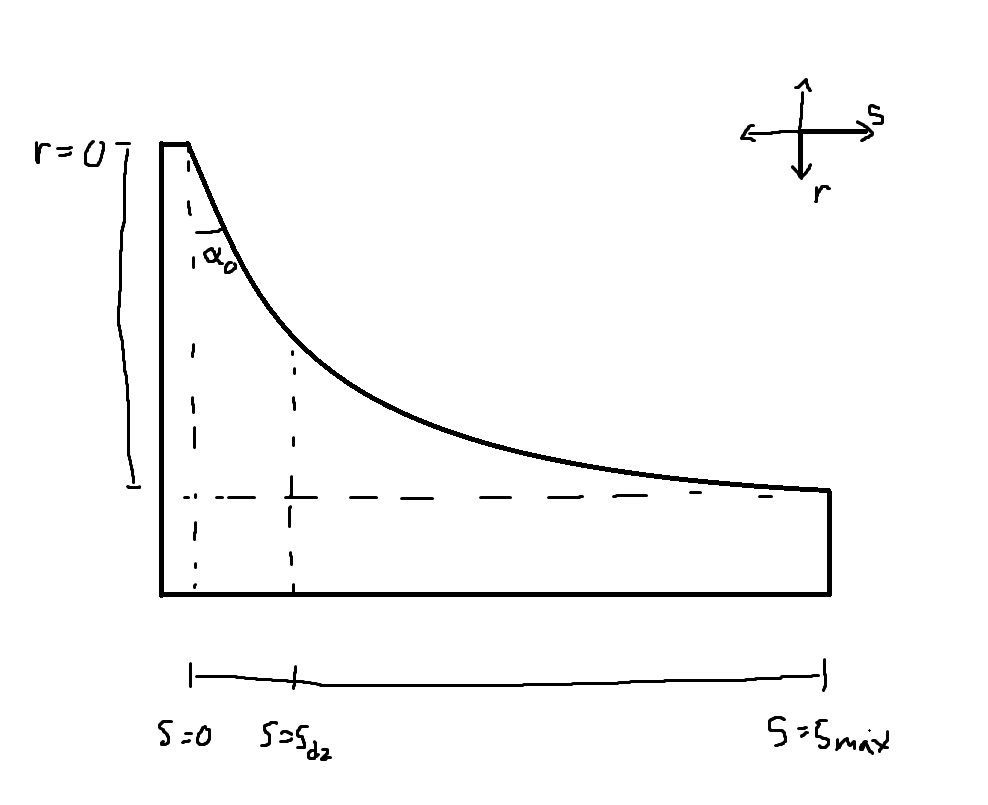
\includegraphics[width=\linewidth]{./illustrations/pulleyForces/primary_ramp_definition.png}
\end{minipage}
\hfill
\begin{minipage}[t]{0.48\textwidth}
\centering
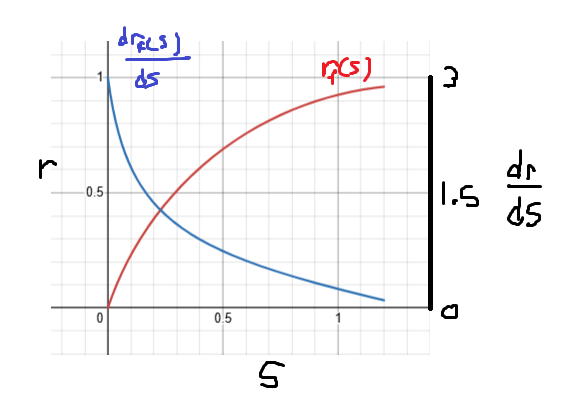
\includegraphics[width=\linewidth]{./illustrations/pulleyForces/radius_wrt_s_function.png}
\end{minipage}
\caption{
Primary ramp geometry.
\textbf{Left:} As axial displacement $s$ increases, the flyweight slides along
the ramp, producing radial change $dr_f$. The instantaneous ramp angle satisfies
$\tan\alpha_p = dr_f/ds$.
\textbf{Right:} Example profiles of $r_f(s)$ and its slope $dr_f/ds$.
}
\label{fig:primary_ramp}
\end{figure}

\paragraph{Primary Admissibility Conditions}

In order to be a valid primary ramp profile $r_f(s)$, it must satisfy:

\begin{enumerate}
    \item $r_f(s) \in C^1([0,s_{\max}])$ (continuously differentiable),
    \item $\dfrac{dr_f}{ds} \ge 0$ over $[0, s_{\max}]$,
    \item $\dfrac{dr_f}{ds}$ is finite over $[0, s_{\max}]$.
\end{enumerate}

Condition (1) ensures the ramp angle $\alpha_p(s)$ is well-defined and
continuous. Condition (2) guarantees that increasing axial displacement
does not reduce flyweight radius. Condition (3) ensures the ramp angle
remains strictly below $\pi/2$ and the axial gain $\tan\alpha_p$ remains finite.

% --------------------------------------------------------------
\paragraph{Secondary Helix Geometry (Axial-to-Rotation Mapping)}

On the secondary pulley, axial travel produces relative rotation
of a helical ramp mechanism, loading a torsional spring and generating
torque-reactive clamping (see \Fig{fig:secondary_helix_def}).

We parameterize this kinematically as
\begin{equation}
\theta_s = \theta_s(s),
\label{eq:secondary_theta_profile}
\end{equation}
where $\theta_s(s)$ is the helix-induced rotation.

An incremental rotation $d\theta_s$ corresponds to a circumferential
displacement $r_h d\theta_s$ along a cylindrical surface of effective
radius $r_h$. The instantaneous secondary helix angle is denoted by
$\alpha_s(s)$ and is defined from the local slope of the ramp surface:

\[
\tan\alpha_s
=
\frac{\text{axial rise}}{\text{circumferential run}}
=
\frac{ds}{r_h d\theta_s}.
\]

Rewriting in differential form gives
\begin{equation}
\tan\alpha_s(s)
=
\frac{1}{r_h \, \dfrac{d\theta_s}{ds}}.
\label{eq:alpha_secondary_inverse_slope}
\end{equation}

Thus, a shallower helix (smaller $\alpha_s$) produces greater rotation
per unit axial travel, while a steeper helix produces less rotation.
This inverse relationship arises naturally from the geometry of motion
on a cylindrical surface.

\begin{remarkbox}[Remark (Contrast with Primary Ramp)]
The primary ramp behaves like a simple wedge: radial displacement is
directly proportional to axial travel, so the ramp angle is naturally
defined by $\tan\alpha_p = dr_f/ds$.

The secondary mechanism instead behaves like a power screw.
Axial motion is produced through rotation around a cylindrical surface,
so the relevant geometric ratio is how much rotation occurs per unit
axial travel. This leads to the slope definition
$ds/(r_h d\theta_s)$ and the inverse relationship in
\Eq{eq:alpha_secondary_inverse_slope}.

In short, the primary redirects force through a wedge,
while the secondary converts torque through a screw-like helix.
The difference is purely geometric and reflects the distinct
mechanisms by which axial motion is generated.
\end{remarkbox}

\begin{figure}[H]
\centering
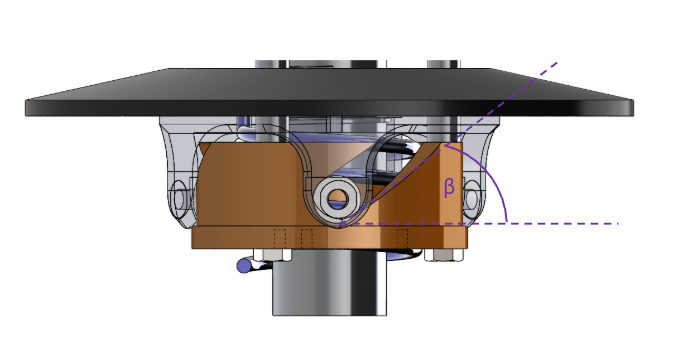
\includegraphics[width=0.7\linewidth]{./illustrations/pulleyForces/secondary_helix_torque_to_axial.png}
\caption{
Secondary helix geometry. Axial travel $s$ induces rotation
$\theta_s(s)$ around a cylindrical surface of radius $r_h$.
The instantaneous helix angle satisfies
$\tan\alpha_s = ds/(r_h d\theta_s)$.
}
\label{fig:secondary_helix_def}
\end{figure}

\paragraph{Secondary Admissibility Conditions}

The helix rotation mapping $\theta_s(s)$ must satisfy:

\begin{enumerate}
    \item $\theta_s(s) \in C^1([0,s_{\max}])$ (continuously differentiable),
    \item $\dfrac{d\theta_s}{ds} \ge 0$ over $[0, s_{\max}]$,
    \item $\dfrac{d\theta_s}{ds}$ is finite over $[0, s_{\max}]$.
\end{enumerate}

Condition (1) ensures the torque-to-axial conversion remains continuous.
Condition (2) guarantees that increasing axial displacement increases
rotation. Condition (3) ensures the effective helix angle
remains strictly below $\pi/2$ and the geometric gain remains finite.

\begin{remarkbox}[Remark (Piecewise Profiles in Practice)]
The $C^1$ requirement above is sufficient for all derivations in this document.
In practice, piecewise $C^1$ profiles (continuous everywhere, continuously
differentiable except at finitely many junction points where left and right
derivatives exist) are also admissible for numerical simulation. At junction
points, one-sided derivatives provide the required slope values, and the
resulting force discontinuities pose no difficulty for standard ODE solvers.
However, large slope discontinuities can introduce local stiffness into the
system: the abrupt change in force gradients may require adaptive solvers to
reduce the timestep significantly near the junction, degrading computational
efficiency. In extreme cases, explicit integrators may struggle to maintain
stability without impractically small step sizes, and implicit or stiff-aware
solvers may be preferable.
\\

Derivations for common ramp and helix profiles are provided in
Appendix~\ref{sec:appendix-ramp-profiles}.
\end{remarkbox}


\subsection{Primary Axial Force Model}\label{sec:primary-axial}

The primary axial clamping force is generated by the interaction
between centrifugal loading of the flyweights and the restoring
force of the primary compression spring.

As shown in \Fig{fig:primary_cvt_3d}, each flyweight of mass $m_f$
rotates with angular speed $\omega_p$ and experiences an outward
radial centrifugal force. This radial force acts along the ramp
profile $r_f(s)$ and is redirected into an axial closing force
through the ramp geometry described in \Sec{sec:ramp-geometry}.

Opposing this motion is the primary compression spring, characterized
by stiffness $k_p$ and preload $x_{p,0}$. As the sheaves close
($s$ increases), the spring compresses and produces a restoring
axial force resisting further closure.

The net axial force on the movable primary sheave is therefore
the axial component of the ramp-redirected centrifugal force
minus the spring force. This net force determines the axial
acceleration $\ddot{s}$ of the primary assembly.

\begin{figure}[H]
\centering

\includegraphics[width=0.7\linewidth]{./illustrations/pulleyForces/primary_cvt_mechanisms.png}
\caption{Primary CVT assembly showing flyweight mass $m_f$, ramp profile $r_f(s)$,
compression spring with stiffness $k_p$ and preload $x_{p,0}$, and axial shift
coordinate $s$.}
\label{fig:primary_cvt_3d}
\end{figure}

The state variable governing primary rotation is $\omega_p$.
\paragraph{Centrifugal Loading of Flyweights}

From \theoryRef{th:centrifugal_force},

\[
F_c = m \omega^2 r.
\]

Let
\begin{itemize}
    \item $m_f$ denote the flyweight mass,
    \item $r_{f,0}$ denote the initial flyweight radius at $s=0$,
    \item $r_f(s)$ denote the incremental radial change produced by the ramp.
\end{itemize}

The total effective flyweight radius is therefore

\[
r_{f,\text{tot}}(s)
=
r_{f,0} + r_f(s).
\]

The radial centrifugal force is

\begin{equation}
F_{p,\mathrm{rad}}(s,\omega_p)
=
m_f \omega_p^2 \big(r_{f,0} + r_f(s)\big).
\label{eq:primary_radial}
\end{equation}

\paragraph{Radial-to-Axial Projection}

The ramp redirects radial force into axial force.
As shown in \Fig{fig:primary_ramp_centrifugal_force},
the axial component of a force acting along the ramp is obtained by

\begin{equation}
F_{p,\mathrm{axial\;component}}
=
F_{p,\mathrm{rad}} \tan\alpha_p(s).
\label{eq:primary_projection}
\end{equation}

From \Eq{eq:alpha_primary_from_slope}, the ramp angle satisfies

\[
\tan\alpha_p(s) = \frac{dr_f}{ds}.
\]

Substituting gives

\begin{equation}
F_{p,\mathrm{cent}}(s,\omega_p)
=
m_f \omega_p^2 \big(r_{f,0} + r_f(s)\big)
\frac{dr_f}{ds}.
\label{eq:primary_centrifugal_axial}
\end{equation}

Thus the axial gain of centrifugal force is governed
by the local ramp slope, while the centrifugal magnitude
depends on the total flyweight radius.

\begin{figure}[H]
\centering
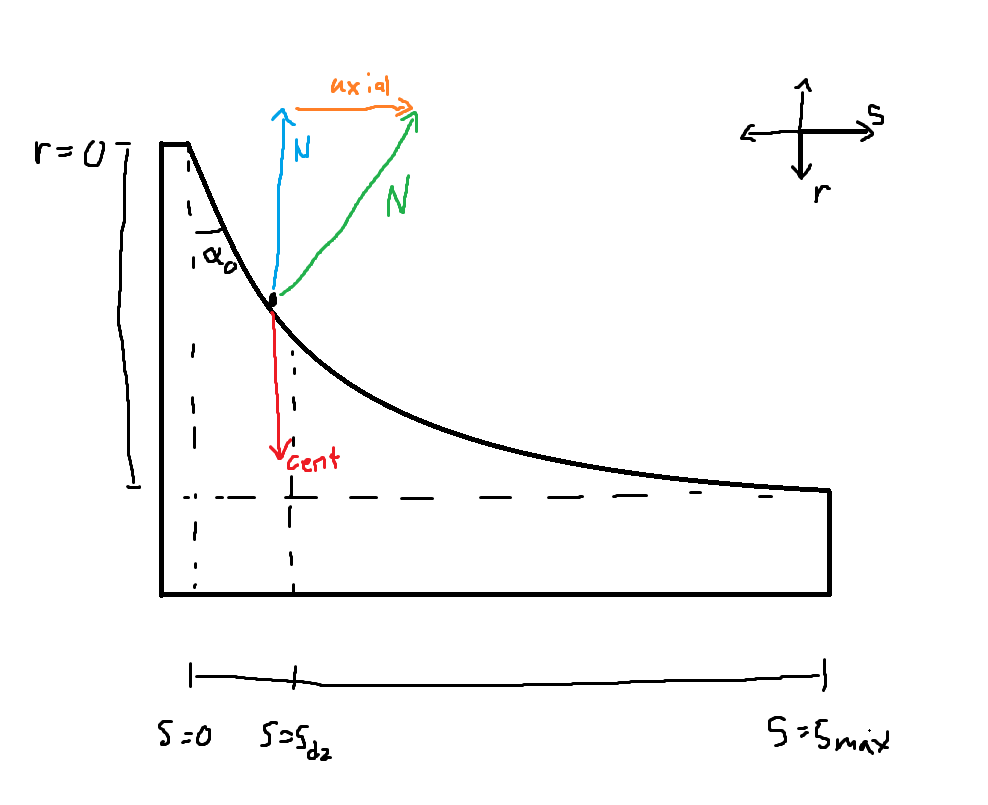
\includegraphics[width=0.7\linewidth]{./illustrations/pulleyForces/primary_ramp_centrifugal_force.png}
\caption{Primary ramp geometry. Radial centrifugal force is redirected
into axial force through the ramp. The projection introduces a factor
of $\tan\alpha_p$, which equals $dr_f/ds$ by definition of the ramp slope.}
\label{fig:primary_ramp_centrifugal_force}
\end{figure}

% --------------------------------------------------------------
\paragraph{Primary Compression Spring}

From \theoryRef{th:hooke_linear},

\[
F = k \Delta x.
\]

Let $k_p$ denote primary stiffness and $x_{p,0}$ preload.

\begin{equation}
F_{p,\mathrm{spring}}(s)
=
k_p (x_{p,0}+s).
\label{eq:primary_spring}
\end{equation}

% --------------------------------------------------------------
\paragraph{Net Primary Axial Force}

The net axial force generated by the primary mechanism is the difference between
the centrifugal axial component and the spring force:

\bigeq{eq:primary_axial}{Primary Axial Force}{
F_{p,\mathrm{ax}}(s,\omega_p)
=
m_f \omega_p^2 \big(r_{f,0} + r_f(s)\big)\frac{dr_f}{ds}
-
k_p (x_{p,0}+s).
}

% ==============================================================
% ==============================================================
\subsection{Secondary Axial Force Model}\label{sec:secondary-axial}

The secondary pulley is \emph{torque-reactive}: its axial clamping force
is generated in response to torque transmitted through the CVT.
Unlike the primary, which produces clamping based on rotational speed,
the secondary produces clamping primarily when torque flows through it.

The mechanism consists of a helical ramp between the two sheaves and a
single spring located between them. This spring serves two roles:
\begin{itemize}
    \item It acts axially in compression as the sheaves separate.
    \item It resists relative rotation torsionally as the helix turns.
\end{itemize}

Thus, axial motion and rotational motion of the helix both load the same spring.

\begin{figure}[H]
\centering
%\includegraphics[width=0.7\linewidth]{./illustrations/secondary_cvt_3d_model_placeholder.png}
\caption{Secondary CVT assembly showing the helix mechanism and spring.
Torque $\tau_s$ transmitted through the belt produces tangential force at
the helix ramps, which is redirected into axial clamping force.}
\label{fig:secondary_cvt_3d}
\end{figure}

% --------------------------------------------------------------
% --------------------------------------------------------------
\paragraph{Physical Mechanism (Screw Analogy)}

The secondary helix behaves mechanically like a screw.

If you try to spin a screw in free space, nothing happens axially.
If you spin a screw into a block that is not restrained, the block
simply rotates with the screw—again producing no axial force.
Axial force only develops when there is resistance to rotation
on one side while torque is applied on the other.

In other words, a screw converts \emph{reacted torque} into axial force.

The secondary helix operates on the same principle.
The belt applies a driving torque to the secondary pulley.
If the driven shaft were free, the entire assembly would rotate
without developing tangential reaction force at the helix.
However, when the driven load resists rotation,
torque is transmitted through the helix ramps.

Those ramps are inclined surfaces—just like screw threads.
As torque attempts to rotate one helix face relative to the other,
contact forces develop along the inclined surfaces.
Because the surfaces are angled, this tangential reaction force
has an axial component.

The result is axial clamping force.

The key distinction from a conventional screw is direction:
in a normal screw, torque pulls two components together.
In the CVT helix, the orientation of the ramp is such that
torque causes the movable sheave to be pushed outward,
increasing belt clamping.

Thus, the secondary does not clamp because it spins.
It clamps because torque is being transmitted and resisted.

% --------------------------------------------------------------
\paragraph{Definition of Transmitted Torque}

Let $\tau_s$ denote the torque transmitted through the secondary shaft.
This is the torque carried from the belt, through the helix mechanism,
and into the driven load.

For the present derivation, $\tau_s$ is treated as a known input.
Its value will be computed later in \Sec{sec:torque-coupling}.

% --------------------------------------------------------------
% --------------------------------------------------------------
\paragraph{Torsional Spring Torque}

As the helix rotates relative to the opposing sheave,
the spring is twisted torsionally.

From \theoryRef{th:hooke_torsional},

\[
\tau = k \Delta \theta.
\]

Let $k_{s,\theta}$ denote torsional stiffness and $\theta_{s,0}$ preload.

\begin{equation}
\tau_{s,\mathrm{spring}}(s)
=
k_{s,\theta}\big(\theta_{s,0}+\theta_s(s)\big).
\label{eq:secondary_torsion}
\end{equation}

This torsional component of the same spring contributes
to helix loading even when no torque is transmitted
($\tau_s = 0$), providing baseline clamping.

% --------------------------------------------------------------
\paragraph{Total Torque Applied to Helix}

\begin{equation}
\tau_{s,\mathrm{total}}
=
\tau_s + \tau_{s,\mathrm{spring}}(s).
\label{eq:secondary_total_torque}
\end{equation}

Both contributions act in the same rotational direction at the helix.
The transmitted torque loads the helix through belt force,
and the torsional spring resists relative rotation.
Both therefore generate axial clamping through the same geometry.

% --------------------------------------------------------------
\paragraph{Torque-to-Axial Conversion Through the Helix}

From \theoryRef{th:torque_definition},

\[
\tau = F_t r_h
\quad\Rightarrow\quad
F_t = \frac{\tau_{s,\mathrm{total}}}{r_h}.
\]

The tangential force $F_t$ acts along two symmetric helix ramp faces.
Each ramp carries half of the total tangential load, introducing
the factor of $1/2$ in the axial projection below.

From helix geometry (see \Fig{fig:secondary_helix_torque_to_axial}),

\begin{equation}
F_{s,\mathrm{helix}}
=
\frac{F_t}{2\tan\alpha_s(s)}.
\label{eq:secondary_projection}
\end{equation}

Substituting $F_t$ and using
\[
\tan\alpha_s(s)
=
\frac{1}{r_h\,\dfrac{d\theta_s}{ds}}
\]
gives

\begin{equation}
F_{s,\mathrm{helix}}(s,\tau_s)
=
\frac{\tau_{s,\mathrm{total}}}{2}
\frac{d\theta_s}{ds}.
\label{eq:secondary_helix_force}
\end{equation}

Notably, the helix radius $r_h$ cancels: torque is converted into
axial force according to the geometric rotation-per-travel
relationship $d\theta_s/ds$, consistent with screw mechanics.

TODO: Remark on less friction at bigger radius if being considered

\begin{figure}[H]
\centering
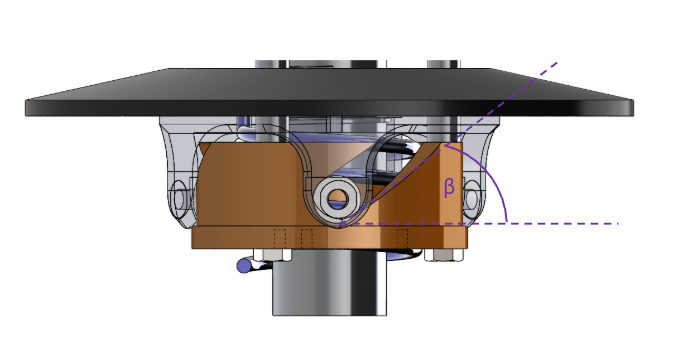
\includegraphics[width=0.7\linewidth]{./illustrations/pulleyForces/secondary_helix_torque_to_axial.png}
\caption{Helix free-body concept. Tangential force from shaft torque is
redirected into axial force along the inclined ramps. Two symmetric
ramp faces share the tangential load, producing the $1/2$ factor.}
\label{fig:secondary_helix_torque_to_axial}
\end{figure}

% --------------------------------------------------------------
\paragraph{Secondary Compression Spring}

The same spring also acts axially between the sheaves.
At $s=0$, the spring is pre-compressed by an amount $x_{s,0}$,
producing a baseline separating force that assists upshift.

As the sheaves move apart (increasing $s$),
the spring extends and its compression decreases.

From \theoryRef{th:hooke_linear},

\[
F = k \Delta x.
\]

Let $k_{s,x}$ denote axial stiffness.  
Because increasing $s$ increases compression,
the effective compression is

\[
\Delta x = x_{s,0} + s.
\]

Thus,

\begin{equation}
F_{s,\mathrm{comp}}(s)
=
k_{s,x}(x_{s,0} + s).
\label{eq:secondary_comp_spring}
\end{equation}

This axial spring force assists upshift at small $s$,
but weakens progressively as the sheaves separate.

% --------------------------------------------------------------
\paragraph{Net Secondary Axial Force}

The total secondary axial force is the sum of:

\begin{itemize}
    \item Helix-generated torque-reactive clamping,
    \item Torsional spring contribution (through the helix),
    \item Direct axial compression spring force.
\end{itemize}

\bigeq{eq:secondary_axial}{Secondary Axial Force}{
F_{s,\mathrm{ax}}(s,\tau_s)
=
\underbrace{
\frac{
\tau_s
+
k_{s,\theta}\big(\theta_{s,0}+\theta_s(s)\big)
}{2}
\frac{d\theta_s}{ds}
}_{\text{torque-reactive helix (including torsional spring)}}
+
\underbrace{
k_{s,x}(x_{s,0}+s)
}_{\text{axial spring}}.
}

% ==============================================================
\subsection{Belt Centrifugal Force on the Wrap}\label{sec:belt-centrifugal}

In addition to the actuator and spring forces derived previously, the belt
itself generates centrifugal loading as it rotates around each pulley.
This section derives the resulting contribution to axial clamping force.

Throughout this sub-section, let
\[
j \in \{p,s\}
\]
denote either pulley, where \(j=p\) corresponds to the primary and
\(j=s\) corresponds to the secondary.

% --------------------------------------------------------------
\paragraph{Centrifugal Force Formulation}

From \theoryRef{th:centrifugal_force}, a mass $m$ rotating at angular velocity
$\omega$ at radius $r$ experiences centrifugal force

\[
F_c = m \omega^2 r.
\]

To apply this to the belt wrapped around a pulley, we require:
\begin{enumerate}
    \item The radius at which this mass rotates.
    \item The mass of belt material in contact with the pulley.
    \item The angular velocity of the belt mass.
\end{enumerate}

Each of these quantities is derived below.

% --------------------------------------------------------------
\subsection{Belt Centrifugal Force on the Wrap}
\label{sec:belt-centrifugal}

In addition to the actuator and spring forces derived previously, the belt
itself generates centrifugal loading as it rotates around each pulley.
This section derives the resulting contribution to axial clamping force.

Throughout this section, let
\[
j \in \{p,s\}
\]
denote either pulley, where \(j=p\) corresponds to the primary and
\(j=s\) corresponds to the secondary.

From \theoryRef{th:centrifugal_force}, a mass \(m\) rotating at angular velocity
\(\omega\) at radius \(r\) experiences centrifugal force

\[
F_c = m\omega^2 r.
\]

To apply this to the belt wrapped around pulley \(j\), three quantities must be defined:

\begin{enumerate}
    \item the radius at which the belt mass rotates,
    \item the mass of belt material carried around the wrap,
    \item the angular velocity of that belt mass.
\end{enumerate}

Each is developed below.

% --------------------------------------------------------------
\paragraph{1. Radius at Which the Belt Mass Rotates}

Centrifugal force acts at the center of mass of the rotating belt element,
not at the outer or inner belt surface. The location of this center of mass
therefore determines the radius that must be used in the centrifugal force
calculation.

The belt cross-section is approximated as a trapezoid
(see \Fig{fig:belt_cross_section_placeholder}) with:

\begin{itemize}
    \item radial thickness \(h_b\),
    \item outer width \(b_{\mathrm{out}}\),
    \item inner width \(b_{\mathrm{in}}\).
\end{itemize}

\begin{figure}[H]
\centering

\includegraphics[width=0.55\linewidth]{./illustrations/pulleyForces/belt_cross_section.png}
\caption{Trapezoidal belt cross-section. The outer width \(b_{\mathrm{out}}\) corresponds
to the surface away from the pulley axis; the inner width \(b_{\mathrm{in}}\) corresponds
to the surface closer to the axis. The radial thickness is \(h_b\).}
\label{fig:belt_cross_section_placeholder}
\end{figure}

The cross-sectional area of the trapezoid is

\begin{equation}
A_b
=
\frac{h_b}{2}\left(b_{\mathrm{out}} + b_{\mathrm{in}}\right).
\label{eq:Ab_trap}
\end{equation}

Let \(y\) denote radial distance measured inward from the outer surface,
so that \(y=0\) at the outer surface and \(y=h_b\) at the inner surface.
For a trapezoid with linear sidewalls, the local width varies linearly with \(y\):

\begin{equation}
b(y)
=
b_{\mathrm{out}}
+
\frac{b_{\mathrm{in}} - b_{\mathrm{out}}}{h_b}y.
\label{eq:belt_width_linear}
\end{equation}

The centroid location \(\Delta r_{\mathrm{cm}}\), measured inward from the
outer surface, follows from the area-centroid definition:

\begin{equation}
\Delta r_{\mathrm{cm}}
=
\frac{1}{A_b}
\int_0^{h_b} y\,b(y)\,\dd y.
\label{eq:delta_r_cm_def}
\end{equation}

Substituting \Eq{eq:belt_width_linear} into \Eq{eq:delta_r_cm_def} gives

\begin{align}
\int_0^{h_b} y\,b(y)\,\dd y
&=
\int_0^{h_b}
y\left(
b_{\mathrm{out}}
+
\frac{b_{\mathrm{in}} - b_{\mathrm{out}}}{h_b}y
\right)\dd y
\nonumber\\[6pt]
&=
\int_0^{h_b} b_{\mathrm{out}} y\,\dd y
+
\frac{b_{\mathrm{in}} - b_{\mathrm{out}}}{h_b}
\int_0^{h_b} y^2\,\dd y
\nonumber\\[6pt]
&=
\frac{h_b^2}{2}b_{\mathrm{out}}
+
\frac{h_b^2}{3}\left(b_{\mathrm{in}} - b_{\mathrm{out}}\right)
\nonumber\\[6pt]
&=
\frac{h_b^2}{6}
\left(b_{\mathrm{out}} + 2b_{\mathrm{in}}\right).
\label{eq:centroid_integral_steps}
\end{align}

Dividing by the area from \Eq{eq:Ab_trap} yields

\begin{equation}
\Delta r_{\mathrm{cm}}
=
h_b\,
\frac{b_{\mathrm{out}} + 2b_{\mathrm{in}}}
{3\left(b_{\mathrm{out}} + b_{\mathrm{in}}\right)}.
\label{eq:delta_r_cm_trap}
\end{equation}

For pulley \(j\), let \(r_{j,\mathrm{out}}(s)\) denote the outer belt radius.
The radius at which the belt mass rotates is therefore

\begin{equation}
r_{j,\mathrm{cm}}(s)
=
r_{j,\mathrm{out}}(s) - \Delta r_{\mathrm{cm}}.
\label{eq:rj_cm_definition}
\end{equation}

% --------------------------------------------------------------
\paragraph{2. Mass of Belt Material on the Wrap}

To determine the centrifugal loading on pulley \(j\), we next determine
the amount of belt mass associated with an infinitesimal portion of its wrap.

Let \(\theta\) denote the angular coordinate measured from the center of the wrap,
so that the wrapped region on pulley \(j\) spans

\[
\theta \in \left[-\frac{\phi_j}{2},\;\frac{\phi_j}{2}\right],
\]

where \(\phi_j(s)\) is the total wrap angle on pulley \(j\)
(see \Fig{fig:belt_centrifugal_wrap_placeholder}).

\begin{figure}[H]
\centering
\includegraphics[width=0.55\linewidth]{./illustrations/pulleyForces/belt_element.png}
\caption{Belt wrapped around pulley \(j\). A differential element at angle \(\theta\)
has arc length \(\dd\ell = r_{j,\mathrm{cm}}\,\dd\theta\) and experiences radially
outward centrifugal force.}
\label{fig:belt_centrifugal_wrap_placeholder}
\end{figure}

A differential belt element subtending angle \(\dd\theta\) at the
mass-centroid radius \(r_{j,\mathrm{cm}}\) has arc length

\[
\dd \ell = r_{j,\mathrm{cm}}\,\dd\theta.
\]

Since the belt has cross-sectional area \(A_b\), the differential belt
element has volume

\begin{equation}
\dd V_j
=
A_b\,\dd\ell.
\label{eq:dV_belt_wrap_j}
\end{equation}

Substituting \(\dd\ell = r_{j,\mathrm{cm}}\,\dd\theta\) gives

\begin{equation}
\dd V_j
=
A_b\,r_{j,\mathrm{cm}}\,\dd\theta.
\label{eq:dV_belt_wrap_j_expanded}
\end{equation}

Let \(\rho_b\) denote the belt material density
(\si{\kilogram\per\meter\cubed}). The corresponding differential mass is then

\begin{align}
\dd m_j
&=
\rho_b\,\dd V_j
\nonumber\\[6pt]
&=
\rho_b A_b\,r_{j,\mathrm{cm}}\,\dd\theta.
\label{eq:dm_belt_wrap_j}
\end{align}

This gives the amount of belt material associated with an infinitesimal
portion of the wrap on pulley \(j\).

% --------------------------------------------------------------
\paragraph{3. Angular Velocity of the Belt Mass}

The rotating belt mass on pulley \(j\) must also be assigned an angular speed.
From \Sec{sec:state}, \(\hat{v}_b\) denotes the modeled belt transport speed. 
The corresponding angular velocity of the belt mass centroid
on pulley \(j\) is then

\begin{equation}
\omega_{b,j}
=
\frac{\hat{v}_b}{r_{j,\mathrm{cm}}(s)}.
\label{eq:omega_bj_definition}
\end{equation}

This relation expresses the fact that the same belt transport speed corresponds
to different local angular velocities depending on the radius of motion. 
The evolution of \(\hat{v}_b\) is derived later in \Sec{sec:torque-coupling}.

% --------------------------------------------------------------
\paragraph{Distributed Centrifugal Load Along the Wrap}

With the radius, differential mass, and angular velocity now defined,
the centrifugal force on the differential belt element follows from
\theoryRef{th:centrifugal_force}:

\begin{align}
\dd F_{c,j}
&=
\dd m_j\,\omega_{b,j}^2\,r_{j,\mathrm{cm}}
\nonumber\\[6pt]
&=
\left(\rho_b A_b\,r_{j,\mathrm{cm}}\,\dd\theta\right)
\left(\frac{\hat{v}_b}{r_{j,\mathrm{cm}}}\right)^2
r_{j,\mathrm{cm}}
\nonumber\\[6pt]
&=
\rho_b A_b\,\hat{v}_b^2\,\dd\theta.
\label{eq:dFc_belt_j}
\end{align}

This force acts radially outward at each point along the wrap.

% --------------------------------------------------------------
\paragraph{Total Radial Force Over the Wrap}

Integrating \Eq{eq:dFc_belt_j} over the full wrap angle gives the total
radially-directed centrifugal force on pulley \(j\):

\begin{align}
F_{c,j,\mathrm{rad}}
&=
\int_{-\phi_j/2}^{\phi_j/2}
\rho_b A_b\,\hat{v}_b^2\,\dd\theta
\nonumber\\[6pt]
&=
\rho_b A_b\,\hat{v}_b^2
\int_{-\phi_j/2}^{\phi_j/2}\dd\theta
\nonumber\\[6pt]
&=
\rho_b A_b\,\hat{v}_b^2\,\phi_j(s).
\label{eq:Fc_rad_wrap_j}
\end{align}

% --------------------------------------------------------------
\paragraph{Radial-to-Axial Conversion Through the Sheave Cone}

The radial centrifugal force acts outward against the conical sheave faces.
Because the sheaves are inclined at cone half-angle \(\beta\), radial loading
cannot occur without simultaneous axial motion of the sheaves.
Thus, a purely radial force applied to the belt generates an axial
reaction component that contributes to clamping.

From the pulley geometry derived previously (see \Eq{eq:cone_geometry_diff}),
the relationship between radial and axial displacement in the active
shift region is

\[
\frac{\dd r}{\dd s}
=
\frac{1}{2\tan\beta}.
\]

For an infinitesimal displacement,

\[
\delta W
=
F_{\mathrm{rad}}\,\dd r
=
F_{\mathrm{ax}}\,\dd s.
\]

Substituting \(\dd r = \dfrac{1}{2\tan\beta}\dd s\) gives

\[
F_{\mathrm{rad}}\,
\frac{1}{2\tan\beta}\dd s
=
F_{\mathrm{ax}}\,\dd s.
\]

Canceling \(\dd s\) yields

\[
F_{\mathrm{ax}}
=
\frac{F_{\mathrm{rad}}}{2\tan\beta}.
\]

Thus, the axial clamping contribution from belt centrifugal force on pulley \(j\) is

\begin{equation}
F_{c,j}
=
\frac{
\rho_b A_b\,\hat{v}_b^2\,\phi_j(s)
}{
2\tan\beta
}.
\label{eq:Fcj_general}
\end{equation}

% ==============================================================
\subsection{Axial Shift Dynamics}\label{sec:shift-dyn}

Earlier (see \Eq{eq:axial_newton_base}),
the evolution of the shift coordinate was established as

\begin{equation}
m\,\ddot{s}
=
F_{p,\text{ax}} - F_{s,\text{ax}},
\label{eq:axial_newton_base_recall}
\end{equation}

where $F_{p,\text{ax}}$ and $F_{s,\text{ax}}$ are the axial forces
generated by the primary and secondary mechanisms, respectively.

We now complete this model by:
\begin{enumerate}
    \item Expanding the force terms to include centrifugal belt loading,
    \item Replacing the lumped mass $m$ with the equivalent inertia
          associated with coordinated shift motion.
\end{enumerate}

% --------------------------------------------------------------
\paragraph{Equivalent Inertia Associated with $s$}

Newton's second law applies to physical masses in translation.
Since $s$ parameterizes coordinated motion of several bodies,
we construct an equivalent mass $m_{\mathrm{eq}}$ such that the total
kinetic energy associated with shift can be written in the form
of \theoryRef{th:kinetic_energy_trans}:

\[
T_{\text{shift}} = \frac12\,m_{\mathrm{eq}}\,\dot s^2.
\]

The movable primary sheave translates with speed $\dot s$
in the positive coordinate direction.
The movable secondary sheave translates with equal magnitude speed
(but opposite physical direction), so its kinetic energy also contributes
proportionally to $\dot s^2$.

Let $m_{p,m}$ and $m_{s,m}$ denote the masses of the movable
primary and secondary sheaves.

% --------------------------------------------------------------
\paragraph{Belt Mass Contribution}

The total belt mass is

\begin{equation}
m_b = \rho_b A_b L_b,
\label{eq:mb_def}
\end{equation}

where $A_b$ is the trapezoidal cross-sectional area from
\Eq{eq:Ab_trap} and $L_b$ is the constant belt length.

The belt moves continuously with a single belt speed,
but the axial component of that motion associated with
a change in $s$ is determined by geometry.
From the axial-radial coupling in \Eq{eq:drpds_piecewise},
a change in sheave separation $s$ is shared between the two
conical faces supporting the belt wedge.
Thus, the belt's axial velocity relative to the pulley axis is

\begin{equation}
\dot s_b = \frac{\dot s}{2}.
\label{eq:belt_half_speed}
\end{equation}

The kinetic energy associated with this axial motion is therefore

\[
T_b
=
\frac12 m_b \left(\frac{\dot s}{2}\right)^2
=
\frac12 \left(\frac{m_b}{4}\right)\dot s^2.
\]

Expressed in the generalized coordinate $s$,
the belt contributes an effective mass of $m_b/4$.

% --------------------------------------------------------------
\paragraph{Total Equivalent Mass}

The total inertia associated with shift becomes

\begin{equation}
m_{\mathrm{eq}}
=
m_{p,m} + m_{s,m} + \frac{m_b}{4}
=
m_{p,m} + m_{s,m} + \frac{\rho_b A_b L_b}{4}.
\label{eq:meq_def}
\end{equation}

% --------------------------------------------------------------
\paragraph{Net Axial Force in the $s$ Coordinate}

Collecting the axial force contributions derived previously:

\begin{itemize}
  \item $F_{p,\mathrm{ax}}(s,\omega_p)$ from \Eq{eq:primary_axial},
  \item $F_{s,\mathrm{ax}}(s,\tau_s)$ from \Eq{eq:secondary_axial},
  \item $F_{c,p}(s,\hat{v}_b)$ from \Eq{eq:Fcj_general} with $j=p$,
  \item $F_{c,s}(s,\hat{v}_b)$ from \Eq{eq:Fcj_general} with $j=s$.
\end{itemize}

With the sign convention defined above, the generalized force
in the positive $s$ direction is

\begin{equation}
\sum F_s
=
\Big(F_{p,\mathrm{ax}} + F_{c,p}\Big)
-
\Big(F_{s,\mathrm{ax}} + F_{c,s}\Big).
\label{eq:sumF_shift}
\end{equation}

% --------------------------------------------------------------
\paragraph{Shift Equation of Motion}

Applying Newton's second law in the generalized coordinate,

\[
\sum F_s = m_{\mathrm{eq}}\,\ddot s,
\]

and substituting \Eq{eq:meq_def} and \Eq{eq:sumF_shift},
we obtain

\bigeq{eq:s_ddot_final}{Axial Shift Acceleration}{
\ddot s
=
\frac{
\Big(F_{p,\mathrm{ax}}(s,\omega_p) + F_{c,p}(s,v_b)\Big)
-
\Big(F_{s,\mathrm{ax}}(s,\tau_s) + F_{c,s}(s,v_b)\Big)
}{
m_{p,m} + m_{s,m} + \dfrac{\rho_b A_b L_b}{4}
}.
}

\Eq{eq:s_ddot_final} provides the axial shift acceleration
as a function of the current state variables
$(s,\dot s,\omega_p,\omega_s)$ and the reacted secondary torque $\tau_s$.
The remaining coupling between axial and rotational dynamics
enters through $\tau_s$, which will be determined later
using \theoryRef{th:newton-rot}.

% ==============================================================
\subsection{Section Summary and Forward Outlook}\label{sec:axial-summary}

In this section we established a complete axial force model for the CVT
mechanism and derived a closed-form equation of motion for the generalized
shift coordinate $s(t)$.

At this stage, the axial subsystem is formally closed with respect to the
state variables of the model, but it still depends on one remaining
coupling quantity that is not determined internally by the axial force
balance: the reacted secondary torque $\tau_s$.
Although $\tau_s$ appears explicitly in the secondary axial force model,
its value is determined by the rotational dynamics of the drivetrain
and by torque transmission through the belt.
Thus, aside from the shared state variables, the axial and rotational
subsystems are coupled through this torque term.

The next step is to determine how torque is transmitted across the CVT
as a function of pulley radii and speed ratio.
This will establish the relationship between $\tau_s$,
input torque at the primary, and the evolving ratio
$R = r_s / r_p$.
Once this transmission relationship is obtained,
the axial and rotational equations can be combined into a unified,
state-space representation of the full CVT dynamics.

With the axial force structure now complete,
attention turns to the torque transmission mechanism
that closes the remaining dynamical loop.


% ==============================================================
\section{Belt Motion, Torque Transmission, and Contact States}
\label{sec:belt_motion_torque_transmission_contact_states}

The axial force model derived in \Sec{sec:axial} depends on quantities
that are not determined by axial motion alone. These remaining quantities
enter through the belt, which couples the primary and secondary pulleys in
two distinct ways. First, the belt moves through the pulley system with a
transport speed that enters the belt centrifugal loading terms. Second,
through frictional contact with the pulley faces, it transmits tangential
force and therefore torque between the pulleys. The purpose of this section
is to introduce the belt as the coupling medium of the CVT, define the
belt transport motion and torque path through the system, and then
distinguish the stick and slip states that govern transmission behavior.

% ==============================================================
\subsection{The Belt as the Coupling Medium}

The primary and secondary pulleys do not interact directly.
All mechanical interaction between them occurs through the belt.
The belt is therefore the coupling medium of the CVT.

This coupling occurs in two distinct ways.

First, the belt moves through the pulley system with a transport speed.
Because the belt has mass, this motion contributes to the dynamics through
belt-speed-dependent effects such as centrifugal loading.

Second, the belt transmits tangential traction through frictional contact
with the pulley faces. This tangential interaction is what allows torque
to pass from the primary to the secondary.

These two roles are illustrated in \Fig{fig:torque_path}. The primary pulley
drives the belt, the belt moves through the transmission path, and the belt in
turn drives the secondary pulley.

\begin{figure}[H]
    \centering
    
\includegraphics[width=0.8\linewidth]{./illustrations/torque/cvt_overview_forces.png}
    \caption{Belt-mediated coupling in the CVT. The primary pulley applies
    torque to the belt, the belt moves through the transmission path, and the
    belt applies torque to the secondary pulley. Through frictional contact,
    the belt also transmits tangential force between the pulley faces.}
    \label{fig:torque_path}
\end{figure}

To describe this interaction, the following belt-mediated quantities will be used:

\begin{align}
\tau_p &:\ \text{torque applied by the primary pulley onto the belt}, \\
\tau_s &:\ \text{torque applied by the belt onto the secondary pulley}, \\
F_t &:\ \text{effective tangential force transmitted through the belt}, \\
\hat{v}_b &:\ \text{modeled belt transport speed}, \\
\end{align}

The quantities $\tau_p$ and $\tau_s$ describe how torque enters and leaves the
belt transmission path.
The quantity $F_t$ describes the tangential traction carried through the belt.
The quantity $\hat{v}_b$ describes the motion of the belt itself through the
pulley system.

The remainder of this section develops these belt-mediated quantities in order.
We first examine the transport motion of the belt, then the tangential force
and torque path carried through it, and finally the contact states that govern
whether the transmission is in stick or slip.

% ==============================================================
\subsection{Belt Transport Motion}\label{sec:belt_transport_motion}

Before torque transmission can be described, the motion of the belt itself
must be established.

Under \AssRef{assump:constant_belt_length}, the belt is assumed to remain
taut and its total length is fixed. As a result, the belt does not admit
independent local stretching or compression along different portions of its
path. Instead, it moves through the CVT as a single continuous body with one
transport speed at any given instant.

To represent this motion in the dynamic model, let

\[
\hat{v}_b(t)
\]

denote the modeled belt transport speed. This quantity describes the rate at
which belt material moves along the transmission path and is the belt-speed
state introduced in \Sec{sec:state}.

If a belt segment is adhering locally to pulley \(j \in \{p,s\}\), then the
belt speed at that contact must match the circumferential speed of the pulley
at the radius where the belt mass is modeled to move. Using the centroid
radius from \Eq{eq:rj_cm_definition}, the pulley-imposed belt-line speeds are therefore

\begin{equation}
v_{p,\mathrm{cm}}
=
r_{p,\mathrm{cm}}(s)\,\omega_p,
\qquad
v_{s,\mathrm{cm}}
=
r_{s,\mathrm{cm}}(s)\,\omega_s.
\label{eq:belt_line_speeds}
\end{equation}

These quantities represent the belt transport speeds that would be imposed by
the primary and secondary pulleys, respectively, if the belt were adhering
locally at each contact.

If both pulley contacts are adhering simultaneously, then the belt cannot move
at two different speeds at once. The transport speed must therefore satisfy the
compatibility condition

\begin{equation}
\hat{v}_b
=
v_{p,\mathrm{cm}}
=
v_{s,\mathrm{cm}}.
\label{eq:vb_stick_compatibility}
\end{equation}

This is the kinematic condition associated with sticking contact.

If the two pulley-imposed belt-line speeds are unequal, then simultaneous
adherence at both contacts is not kinematically possible. In that case, the
transmission must depart from the sticking condition and enter a slipping
state, which is discussed later in this section.

With the belt transport motion now identified, the next step is to determine
how tangential force and power are carried through this moving belt.


% ==============================================================
\subsection{Belt Power Flow and Torque Transmission}

With the belt transport motion now identified, the next step is to determine
how force and power are carried through the moving belt.

Since the belt is the only mechanical connection between the pulleys, it must
carry the power transmitted through the CVT.

Torque transmission arises from tangential forces acting between the belt and
the pulley faces. Let \(F_t\) denote the effective tangential force transmitted
through the belt.

The mechanical power carried by the belt is therefore

\begin{equation}
P = F_t \,\hat{v}_b.
\label{eq:belt_power}
\end{equation}

Under \AssRef{assump:ideal_cvt_power}, this power is conserved through the
transmission, so that the power entering the belt at the primary equals the
power leaving at the secondary.

The same transmitted tangential force \(F_t\) acts at the effective contact
radius of each pulley. The torques associated with this force are therefore

\begin{align}
\tau_p &= r_{p,\mathrm{eff}} \, F_t, \\
\tau_s &= r_{s,\mathrm{eff}} \, F_t.
\label{eq:torques_from_Ft}
\end{align}

Here, \(r_{p,\mathrm{eff}}\) and \(r_{s,\mathrm{eff}}\) are the effective
contact radii defined by \Eq{eq:primary_effective_radius} and
\Eq{eq:secondary_effective_radius}, respectively. These radii determine the torque produced
by the transmitted tangential force.
Since both torques arise from the same transmitted force, \(F_t\) can be
eliminated directly. From the primary expression,

\begin{equation}
F_t = \frac{\tau_p}{r_{p,\mathrm{eff}}}.
\label{eq:Ft_from_taup}
\end{equation}

Substituting this into the secondary torque relation gives

\begin{equation}
\tau_s
=
r_{s,\mathrm{eff}}
\left(
\frac{\tau_p}{r_{p,\mathrm{eff}}}
\right)
=
\frac{r_{s,\mathrm{eff}}}{r_{p,\mathrm{eff}}}\,\tau_p.
\label{eq:taus_from_taup_intermediate}
\end{equation}

Recalling the geometric definition of the CVT ratio from \Eq{eq:cvt_ratio},

\begin{equation}
R = \frac{r_{s,\mathrm{eff}}}{r_{p,\mathrm{eff}}},
\label{eq:R_eff_repeat}
\end{equation}

it follows that

\begin{equation}
\tau_s = R\,\tau_p.
\label{eq:torque_ratio}
\end{equation}

Thus, the torque carried through the belt scales directly with the current
CVT ratio. The primary and secondary torques are not independent quantities,
but two descriptions of the same belt-mediated transmission process.

This observation motivates the introduction of a single \emph{coupling torque}.

\begin{equation}
\tau_c \equiv \tau_p.
\end{equation}

The corresponding secondary torque is then
\begin{equation}
\tau_s = R \, \tau_c.
\end{equation}

The transmitted torque is thus not a property of either pulley in isolation, but
of the belt--pulley interaction as a whole. The quantities $\tau_p$ and $\tau_s$
represent the primary-side and secondary-side expressions of this same coupling
torque.


\subsection{Transmission Regimes}
\label{sec:transmission_regimes}

The coupling torque $\tau_c$ defined in \Eq{eq:torque_ratio} is the torque
actually transmitted through the belt.
It is not prescribed externally.
Instead, its value depends on the contact state of the transmission.

In \Sec{sec:belt_transport_motion}, the belt was introduced as a moving body
with modeled transport speed $\hat{v}_b$.
That quantity describes the motion of belt material through the CVT and is used
in belt-speed-dependent effects such as centrifugal loading.
The present subsection addresses a different issue: whether the belt is locally
adhering or slipping at the pulley contacts.
For this purpose, the relevant kinematic quantities are the tangential contact
speeds imposed by the pulley surfaces.

\paragraph{No-slip torque.}

If the belt remains adhered at the pulley contacts, then the transmission
behaves as a sticking constraint.
In that case, the transmitted torque is whatever value is required to preserve
that adhered motion.

We denote this required torque by
\begin{equation}
\tau_{\mathrm{ns}},
\end{equation}
where the subscript ``ns'' denotes \emph{no slip}.
Thus, in a sticking state,
\begin{equation}
\tau_c = \tau_{\mathrm{ns}}.
\end{equation}

\paragraph{Traction limits.}

Adherence cannot be maintained for arbitrary transmitted torque.
The belt--pulley contact can only sustain a finite tangential traction, and
therefore only a finite coupling torque.

We therefore introduce directional traction bounds and write the admissible
sticking interval as
\begin{equation}
\tau_- \le \tau_{\mathrm{ns}} \le \tau_+.
\label{eq:stick_admissible_interval}
\end{equation}

If \Eq{eq:stick_admissible_interval} holds, then the no-slip torque lies within
the available traction limits, so sticking is physically admissible.

If instead $\tau_{\mathrm{ns}}$ lies outside this interval, then the torque
required to maintain adherence cannot be supported by the contact, and slip must
occur.

\paragraph{Why a slip metric is still needed.}

The traction condition alone is not enough to determine the regime.
Once slipping has begun, the transmission does not return immediately to stick
simply because $\tau_{\mathrm{ns}}$ later re-enters the admissible interval.
Stick is only recovered once the existing relative motion has decayed to zero.

For this reason, one further quantity is needed: a measure of the relative
contact-speed mismatch.

In analogy with the pulley-imposed belt-line speeds introduced in
\Sec{sec:belt_transport_motion}, define the pulley-imposed tangential contact
speeds at the effective radii by
\begin{equation}
u_p = r_{p,\mathrm{eff}}\omega_p,
\qquad
u_s = r_{s,\mathrm{eff}}\omega_s.
\label{eq:contact_surface_speeds}
\end{equation}

These are the tangential speeds that the primary and secondary pulley surfaces
would impose at their effective contact radii if each were enforcing local
adherence.

Under \AssRef{assump:single_slip_interface}, the model permits slip at only one
pulley contact at a time.
A single scalar mismatch is therefore sufficient:
\begin{equation}
v_{\Delta}
=
u_p - u_s
=
r_{p,\mathrm{eff}}\omega_p
-
r_{s,\mathrm{eff}}\omega_s.
\label{eq:v_delta_def}
\end{equation}

If
\begin{equation}
v_{\Delta}=0,
\label{eq:v_delta_zero}
\end{equation}
then the two pulley motions are compatible with a common adhered contact motion,
so a sticking state is kinematically possible.

If instead
\begin{equation}
v_{\Delta}\neq 0,
\label{eq:v_delta_nonzero}
\end{equation}
then the two pulley contacts are demanding different tangential contact speeds,
and simultaneous adherence at both contacts is not possible.

The sign of $v_{\Delta}$ indicates the slip direction:
if $v_{\Delta}>0$, the primary tends to drive the belt faster than the secondary
is accepting it; if $v_{\Delta}<0$, the opposite is true.

\paragraph{Stick and slip states.}

The transmission can therefore be in stick only when two conditions are
satisfied simultaneously:

\begin{enumerate}
    \item the required no-slip torque lies within the admissible traction
    interval, and
    \item the relative slip velocity has vanished.
\end{enumerate}

This gives the regime structure
\begin{equation}
\tau_c =
\begin{cases}
\tau_{\mathrm{ns}},
&
v_{\Delta}=0
\;\text{and}\;
\tau_- \le \tau_{\mathrm{ns}} \le \tau_+,
\\[10pt]
\text{traction-limited value},
&
\text{otherwise}.
\end{cases}
\label{eq:tau_c_regime_structure}
\end{equation}

\paragraph{Physical interpretation.}

If the required no-slip torque leaves the admissible interval, the contact can
no longer maintain adherence and slip begins.

Once slip is present, the transmission remains on a slip branch until the
existing mismatch has been driven back to zero.
This is why the slip metric is needed in addition to the traction limits:
the traction limits determine whether sticking is admissible, while
$v_{\Delta}$ determines whether slipping is still occurring and, if so, in which
direction. Importantly, this does not determine at \emph{which} contact slip occurs,
only which is overruning the other.


% ==============================================================
\subsection{Regularized Belt-Speed Evolution}
\label{sec:belt_speed_evolution}

The modeled belt transport speed $\hat{v}_b$ introduced in
\Sec{sec:belt_transport_motion} enters the axial force model through the
belt centrifugal terms derived in \Sec{sec:belt-centrifugal}.
Its evolution must therefore be specified as part of the complete dynamic model.

\paragraph{Exact closure in stick.}

From \Eq{eq:belt_line_speeds}, the pulley-imposed belt-line speeds are

\[
v_{p,\mathrm{cm}} = r_{p,\mathrm{cm}}(s)\,\omega_p,
\qquad
v_{s,\mathrm{cm}} = r_{s,\mathrm{cm}}(s)\,\omega_s.
\]

When the transmission is in a sticking state, these two speeds are compatible.
In that case, the belt transport speed is determined exactly by the adhered
kinematics, so that

\begin{equation}
\hat{v}_b = v_{p,\mathrm{cm}} = v_{s,\mathrm{cm}}.
\label{eq:vb_stick_exact}
\end{equation}

Thus, no additional approximation is required while the contacts remain stuck.

\paragraph{Need for a slip closure.}

When the transmission is slipping, the two pulley-imposed belt-line speeds no
longer agree.
At that point, the exact belt transport speed is no longer determined by
kinematic compatibility alone.
A fully resolved treatment would require a simultaneous branch-dependent
solution for contact state, transmitted torque, and adhered belt motion.

Such a closure is beyond the level of detail adopted in the present model.
Instead, the belt transport speed is represented during slip by a regularized
dynamic approximation. This preserves a continuous belt-speed state for use in
belt-speed-dependent terms, while avoiding a substantially more complicated
contact solve.

\paragraph{Regularized target speed.}

To construct this approximation, define the target belt speed

\begin{equation}
v_b^\ast
=
\frac{1}{2}
\left(
v_{p,\mathrm{cm}} + v_{s,\mathrm{cm}}
\right).
\label{eq:vb_target}
\end{equation}

This quantity represents the midpoint of the two pulley-imposed belt-line
speeds and therefore provides a natural reference speed during slip.

\paragraph{Evolution law.}

Outside the sticking regime, the modeled belt speed is evolved toward
\(v_b^\ast\) using the first-order relaxation law

\begin{equation}
\dot{\hat{v}}_b
=
\frac{v_b^\ast - \hat{v}_b}{T_b},
\label{eq:vb_relaxation}
\end{equation}

where \(T_b > 0\) is a belt-speed regularization time constant.

A small value of \(T_b\) causes \(\hat{v}_b\) to track the target speed
rapidly, while a larger value produces a more gradual response.
In either case, \(\hat{v}_b\) remains continuous through transitions between
stick and slip.

\paragraph{Resulting closure.}

The modeled belt transport speed is therefore obtained from the regime-dependent
rule

\begin{equation}
\hat{v}_b =
\begin{cases}
v_{p,\mathrm{cm}} = v_{s,\mathrm{cm}},
&
v_{\Delta}=0
\;\text{and}\;
\tau_- \le \tau_{\mathrm{ns}} \le \tau_+,
\\[10pt]
\text{solution of }
\dot{\hat{v}}_b = \dfrac{v_b^\ast - \hat{v}_b}{T_b},
&
\text{otherwise.}
\end{cases}
\label{eq:vb_regime_law}
\end{equation}

This closure is exact in stick and regularized in slip.
Its purpose is not to resolve the detailed local adhered contact during slip,
but to provide a consistent and continuous modeled belt speed for the
belt-speed-dependent terms already present in the dynamic formulation.


\subsection{Summary and Forward Outlook}

This section established the belt-level quantities required to couple the
axial and rotational subsystems of the CVT model.

The belt was introduced as the mechanical connection between the pulleys,
with two distinct dynamical roles: it transports belt mass through the
system and it transmits tangential force and therefore torque between the
pulley faces. On this basis, the modeled belt transport speed $\hat{v}_b$
and the coupling torque $\tau_c$ were defined, and the stick and slip
regimes governing transmission behavior were identified. A regularized
evolution law for $\hat{v}_b$ was then introduced to close the
belt-speed-dependent terms of the model during slip while preserving exact
kinematic compatibility in stick.

At this stage, the transmission structure has been established, but two
ingredients remain to be determined explicitly: the no-slip torque
$\tau_{\mathrm{ns}}$ and the traction limits $\tau_-$ and $\tau_+$.
The next section derives the no-slip torque required to maintain adhered
motion. The section following that then derives the admissible traction
bounds that determine when sticking can be sustained and when the
transmission must remain on a slip branch.

\section{Derivation of the No-Slip Coupling Torque}
\label{sec:tau_ns}

In \Sec{sec:transmission_regimes}, the coupling torque $\tau_c$ was introduced
as an internal torque whose value depends on the active transmission regime.
The purpose of this section is to derive the explicit form of $\tau_c$ on the
sticking branch, i.e.\ the no-slip torque $\tau_{\mathrm{ns}}$.

We proceed in four steps:

\begin{enumerate}
    \item Write the rotational equations of motion for the primary and secondary pulleys.
    \item Recall the external torque and inertia models on each side.
    \item Impose the no-slip kinematic constraint.
    \item Eliminate angular accelerations to obtain the no-slip coupling torque.
\end{enumerate}

The result is the sticking-branch torque law used later in the regime model.

% --------------------------------------------------------------
\subsection{System Definition and Torque Path}

\begin{figure}[H]
\centering

\includegraphics[width=0.85\linewidth]{./illustrations/torque/cvt_overview_forces.png}
\caption{Torque transmission schematic.
Engine torque $\tau_{\text{eng}}$ drives the primary pulley
(angular velocity $\omega_p$).
Coupling torque $\tau_c$ is transmitted through the belt to the secondary pulley
(angular velocity $\omega_s$).
The secondary delivers torque to the downstream drivetrain,
which resists motion with torque $\tau_{\text{load}}$.}
\label{fig:torque_path}
\end{figure}

We model two rotating bodies:

\begin{itemize}
    \item the primary side, rigidly connected to the engine,
    \item the secondary side, driving the downstream drivetrain and vehicle.
\end{itemize}

The external torques and effective inertias used below are

\begin{itemize}
    \item $\tau_{\text{eng}}(t)$ : engine output torque applied to the primary pulley,
    \item $\tau_{\text{load}}(t)$ : resisting torque reflected to the secondary pulley,
    \item $I_p$ : total rotational inertia of the engine + primary CVT pulley,
    \item $I_s$ : total effective rotational inertia about the secondary pulley.
\end{itemize}

Their explicit models are recalled in the following subsections.
The remaining internal unknown is the transmitted coupling torque $\tau_c(t)$.

% --------------------------------------------------------------
\subsection{Rotational Equations of Motion}

Applying \theoryRef{th:newton-rot} to the primary side gives

\bigeq{eq:primary_rot_dyn}{Primary Pulley Rotational Dynamics}{
\tau_{\text{eng}}(t) - \tau_c(t)
=
I_p\,\dot{\omega}_p(t)
}

Using the secondary-side no-slip torque mapping established in
\Eq{eq:tau_relation}, the secondary rotational equation on the sticking branch is

\bigeq{eq:secondary_rot_dyn}{Secondary Pulley Rotational Dynamics}{
R(t)\tau_c(t) - \tau_{\text{load}}(t)
=
I_s\,\dot{\omega}_s(t)
}

At this point, \Eq{eq:primary_rot_dyn} and \Eq{eq:secondary_rot_dyn}
provide two equations for the three internal unknowns
\[
\dot{\omega}_p(t),\qquad
\dot{\omega}_s(t),\qquad
\tau_c(t).
\]

The remaining quantities appearing in these equations
--- namely the applied torques $\tau_{\text{eng}}(t)$ and $\tau_{\text{load}}(t)$,
the effective inertias $I_p$ and $I_s$, and the geometric ratio $R(t)$ ---
are treated as known inputs, parameters, or previously defined geometric
quantities.
Their explicit forms are recalled in the following subsections.

Thus, the rotational system is not yet closed:
two equations are available for three unknowns.
A third relation is therefore required to determine the coupling torque.
For the no-slip branch, that final relation will come from the sticking
kinematic constraint introduced after the torque and inertia models are stated.

% --------------------------------------------------------------
\subsection{Engine Torque Model}
\label{sec:tau_eng_model}

The engine provides the driving torque
$\tau_{\text{eng}}(t)$ acting on the primary pulley.

In this model, engine output torque is represented as a
user-supplied function of primary angular velocity.
Under the full-throttle assumption
(\AssRef{assump:full_throttle_model}),

\begin{equation}
\tau_{\text{eng}}(t)
=
\tau_{\text{eng}}\!\big(\omega_p(t)\big),
\label{eq:tau_eng_from_curve}
\end{equation}

so torque depends only on instantaneous primary speed.

This representation is consistent with standard engine
characterization, where torque is measured as a function
of crankshaft speed under steady full-load conditions.

% --------------------------------------------------------------
\paragraph{Admissibility Constraints}

The supplied torque function must satisfy:

\begin{itemize}
    \item It is defined over a bounded operating domain
          $\omega_{\min} \le \omega_p \le \omega_{\max}$.
    \item It is finite and real-valued over this domain.
    \item Outside this domain, torque is either saturated
          or $\omega_p$ is constrained to remain within bounds.
\end{itemize}

No specific functional form is required.
The dynamical model only requires the mapping
$\omega_p \mapsto \tau_{\text{eng}}$
to evaluate \Eq{eq:primary_rot_dyn}.

% --------------------------------------------------------------
\paragraph{Example: Kohler CH440 Engine Curve}

As an illustrative example, \Fig{fig:ch440_torque_curve}
shows a representative torque and power curve for the
Kohler CH440 engine.

\begin{figure}[H]
\centering
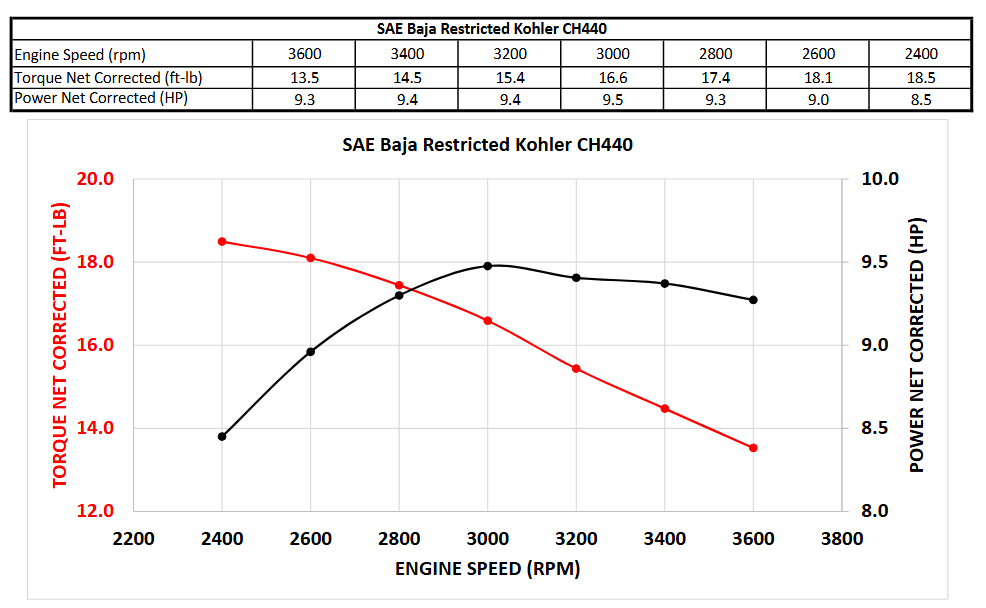
\includegraphics[width=0.75\linewidth]{./illustrations/torque/kohler_ch440_torque_power_curve.png}
\caption{
Representative torque and power curves for the Kohler CH440 engine.
Torque is supplied as a function of angular velocity and serves as
the input mapping in \Eq{eq:tau_eng_from_curve}.
}
\label{fig:ch440_torque_curve}
\end{figure}

In simulation, the discrete curve is interpolated to provide
a continuous admissible torque function over the operating range.

% --------------------------------------------------------------
\subsection{Load Torque Model}
\label{sec:tau_load_model}

The resisting torque $\tau_{\text{load}}(t)$ in
\Eq{eq:secondary_rot_dyn} represents the
longitudinal road load reflected to the secondary pulley.

We proceed in three stages:

\begin{enumerate}
    \item Express vehicle speed in terms of secondary rotation.
    \item Derive the total longitudinal road force.
    \item Reflect that force back to the secondary shaft.
\end{enumerate}

% --------------------------------------------------------------
\paragraph{Kinematic Relations}

Let $r_w$ denote effective wheel rolling radius and
$G>0$ the fixed gear ratio defined by

\[
\omega_s = G\,\omega_w.
\]

Vehicle speed is therefore

\begin{equation}
v(t)
=
r_w \omega_w(t)
=
\frac{r_w}{G}\,\omega_s(t).
\label{eq:v_from_secondary}
\end{equation}

% --------------------------------------------------------------
\paragraph{Longitudinal Road Force}

Using \theoryRef{th:newton-trans},
the total longitudinal resistive force on the vehicle is modeled as

\begin{equation}
F_{\text{road}}
=
F_{\text{rr}}
+
F_{\text{grade}}
+
F_{\text{drag}}.
\label{eq:Froad_total}
\end{equation}

\begin{figure}[H]
\centering
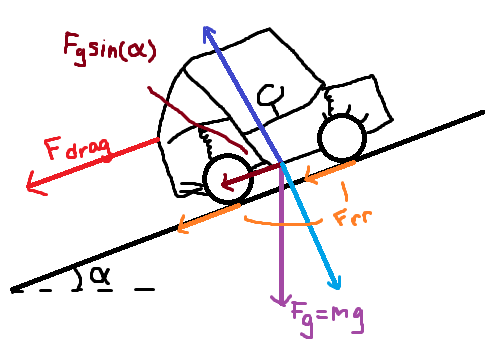
\includegraphics[width=0.75\linewidth]{./illustrations/torque/car_free_body_diagram.png}
\caption{
Free-body diagram of a vehicle on an incline.
The weight $mg$ resolves into $mg\sin\alpha$ along the slope
and $mg\cos\alpha$ normal to the surface.
Rolling resistance and aerodynamic drag oppose motion.
}
\label{fig:car_fbd}
\end{figure}

% --------------------------------------------------------------
\paragraph{Rolling Resistance}

From \theoryRef{th:rolling_resistance},

\begin{equation}
F_{\text{rr}} = C_{\text{rr}}\,N.
\label{eq:Frr_basic}
\end{equation}

From the incline geometry,

\begin{equation}
N = m g \cos\alpha.
\label{eq:normal_force}
\end{equation}

Thus

\begin{equation}
F_{\text{rr}}(v,\alpha)
=
C_{\text{rr}} m g \cos\alpha \;\mathrm{sgn}(v).
\label{eq:Frr_final}
\end{equation}

% --------------------------------------------------------------
\paragraph{Grade Resistance}

From \theoryRef{th:gravity_force}, the gravitational component along the slope is

\begin{equation}
F_{\text{grade}}(\alpha)
=
m g \sin\alpha.
\label{eq:Fgrade}
\end{equation}

% --------------------------------------------------------------
\paragraph{Aerodynamic Drag}

From \theoryRef{th:air_resistance},

\begin{equation}
F_{\text{drag}}(v)
=
\frac12 \rho C_d A_f \, v^2 \,\mathrm{sgn}(v).
\label{eq:Fdrag_final}
\end{equation}

% --------------------------------------------------------------
\paragraph{Total Road Force}

Substituting the above components into
\Eq{eq:Froad_total} yields

\begin{align}
F_{\text{road}}(t)
&=
C_{\text{rr}} m g \cos\alpha
\;\mathrm{sgn}\!\left(v(t)\right)
\nonumber\\
&\quad
+
m g \sin\alpha
\nonumber\\
&\quad
+
\frac12 \rho C_d A_f
\, v(t)^2 \,\mathrm{sgn}\!\left(v(t)\right).
\label{eq:Froad_expanded}
\end{align}

Using \Eq{eq:v_from_secondary},

\[
v(t)
=
\frac{r_w}{G}\,\omega_s(t),
\]

the road force is now fully expressed in terms of the
secondary state variable $\omega_s(t)$.

% --------------------------------------------------------------
\paragraph{Reflection to Secondary Torque}

Wheel torque is

\begin{equation}
\tau_{\text{road},w}(t)
=
r_w F_{\text{road}}(t).
\label{eq:tau_wheel}
\end{equation}

Assuming ideal power transmission
(\AssRef{assump:ideal_cvt_power}),
the resisting torque reflected to the secondary pulley is

\begin{equation}
\tau_{\text{load}}(t)
=
\frac{1}{G}\,\tau_{\text{road},w}(t)
=
\frac{r_w}{G} F_{\text{road}}(t).
\label{eq:tau_load_basic}
\end{equation}

Substituting \Eq{eq:Froad_expanded} gives

\begin{equation}
\boxed{
\tau_{\text{load}}(t)
=
\frac{r_w}{G}
\left[
C_{\text{rr}} m g \cos\alpha
\;\mathrm{sgn}\!\left(\frac{r_w}{G}\omega_s(t)\right)
+
m g \sin\alpha
+
\frac12 \rho C_d A_f
\left(\frac{r_w}{G}\omega_s(t)\right)^2
\mathrm{sgn}\!\left(\frac{r_w}{G}\omega_s(t)\right)
\right].
}
\label{eq:tau_load_final}
\end{equation}

% --------------------------------------------------------------
\subsection{Inertia Definitions}

The rotational equations \Eq{eq:primary_rot_dyn}--\Eq{eq:secondary_rot_dyn}
require the effective rotational inertia about each pulley axis.

% --------------------------------------------------------------
\paragraph{Primary Pulley Inertia}

The primary pulley is rigidly connected to the engine.
All components on this side rotate with angular velocity $\omega_p$,
so no reflection is required.

The effective inertia is therefore the direct sum

\begin{equation}
I_p
=
I_{\text{eng}}
+
I_{\text{prim}},
\label{eq:Ip_def}
\end{equation}

where
\begin{itemize}
    \item $I_{\text{eng}}$ is the engine rotational inertia,
    \item $I_{\text{prim}}$ is the primary CVT pulley inertia.
\end{itemize}

% --------------------------------------------------------------
\paragraph{Secondary Pulley Inertia}

On the secondary side, all downstream components must be
expressed as an equivalent inertia about the secondary axis.

Let

\begin{itemize}
    \item $I_{\text{sec}}$ : secondary CVT pulley inertia,
    \item $I_{\text{gb}}$ : gearbox + intermediate shaft inertia,
    \item $I_{\text{wheel}}$ : wheel + hub inertia about the wheel axis,
    \item $m$ : total vehicle mass,
    \item $r_w$ : effective wheel rolling radius,
    \item $G$ : fixed gear ratio defined by $\omega_s = G\,\omega_w$.
\end{itemize}

% --------------------------------------------------------------
\paragraph{Vehicle Mass as Equivalent Rotational Inertia}

The vehicle’s translational kinetic energy is

\[
T_{\text{trans}}
=
\frac12 m v^2,
\]

with $v = r_w \omega_w$.

Substituting,

\[
T_{\text{trans}}
=
\frac12 m (r_w \omega_w)^2
=
\frac12 (m r_w^2)\,\omega_w^2.
\]

Thus the vehicle mass behaves as an effective rotational inertia

\[
I_{\text{veh,wheel}} = m r_w^2
\]

about the wheel axis.

% --------------------------------------------------------------
\paragraph{Reflection to the Secondary Axis}

Because $\omega_s = G\,\omega_w$,
we have $\omega_w = \omega_s/G$.

Expressing the downstream kinetic energy in terms of $\omega_s$:

\[
T
=
\frac12 I_{\text{wheel}} \left(\frac{\omega_s}{G}\right)^2
+
\frac12 (m r_w^2) \left(\frac{\omega_s}{G}\right)^2.
\]

Factoring,

\[
T
=
\frac12
\left(
\frac{I_{\text{wheel}} + m r_w^2}{G^2}
\right)
\omega_s^2.
\]

Therefore, inertias at the wheel reflect to the secondary pulley as

\[
I_{\text{reflected}}
=
\frac{I_{\text{wheel}} + m r_w^2}{G^2}.
\]

% --------------------------------------------------------------
\paragraph{Total Secondary Inertia}

The total effective inertia about the secondary pulley is

\begin{equation}
I_s
=
I_{\text{sec}}
+
I_{\text{gb}}
+
\frac{I_{\text{wheel}} + m r_w^2}{G^2}.
\label{eq:Is_def}
\end{equation}

Equation \Eq{eq:Is_def} defines the total inertia
opposing angular acceleration of the secondary pulley.

% --------------------------------------------------------------
\subsection{No-Slip Ratio Kinematics}

As established in \Sec{sec:transmission_regimes}, the sticking branch is
characterized by the condition
\[
v_{\Delta}=0,
\]
where \(v_{\Delta}\) was defined in \Eq{eq:v_delta_def} as
\[
v_{\Delta}
=
r_{p,\text{eff}}(t)\,\omega_p(t)
-
r_{s,\text{eff}}(t)\,\omega_s(t).
\]

Setting this equal to zero gives
\begin{equation}
r_{p,\text{eff}}(t)\,\omega_p(t)
=
r_{s,\text{eff}}(t)\,\omega_s(t).
\label{eq:no_slip_condition}
\end{equation}

Using the geometric CVT ratio
\[
R(t)
=
\frac{r_{s,\text{eff}}(t)}{r_{p,\text{eff}}(t)},
\]
\Eq{eq:no_slip_condition} becomes
\begin{equation}
\omega_p(t)=R(t)\,\omega_s(t).
\label{eq:ratio_speed_constraint}
\end{equation}

This is the defining kinematic relation of the sticking branch.
If \Eq{eq:ratio_speed_constraint} does not hold, the present derivation no
longer applies and the transmission must instead be described by the slip
branch.

Differentiating \Eq{eq:ratio_speed_constraint} with respect to time gives
\begin{equation}
\dot{\omega}_p(t)
=
R(t)\,\dot{\omega}_s(t)
+
\omega_s(t)\,\dot R(t),
\label{eq:alpha_relation}
\end{equation}
which is the corresponding acceleration-level compatibility condition.

\subsection{Eliminating Angular Accelerations}

We now combine the primary rotational dynamics
\Eq{eq:primary_rot_dyn},
the secondary rotational dynamics
\Eq{eq:secondary_rot_dyn},
and the no-slip compatibility relation
\Eq{eq:alpha_relation}
to solve for the coupling torque on the sticking branch.

From \Eq{eq:primary_rot_dyn},

\[
\tau_c
=
\tau_{\text{eng}}
-
I_p\,\dot{\omega}_p.
\]

Substituting \Eq{eq:alpha_relation} gives

\begin{equation}
\tau_c
=
\tau_{\text{eng}}
-
I_p\bigl(R\dot{\omega}_s+\omega_s\dot R\bigr).
\label{eq:tau_c_intermediate}
\end{equation}

From \Eq{eq:secondary_rot_dyn},

\[
\dot{\omega}_s
=
\frac{R\tau_c-\tau_{\text{load}}}{I_s}.
\]

Substituting this into \Eq{eq:tau_c_intermediate} gives

\begin{align}
\tau_c
&=
\tau_{\text{eng}}
-
I_p
\left[
R\left(
\frac{R\tau_c-\tau_{\text{load}}}{I_s}
\right)
+
\omega_s\dot R
\right]
\nonumber\\[6pt]
&=
\tau_{\text{eng}}
-
\frac{I_p}{I_s}
\left(
R^2\tau_c-R\tau_{\text{load}}
\right)
-
I_p\omega_s\dot R.
\end{align}

Collecting terms yields

\begin{equation}
\tau_c
\left(
1+\frac{I_p}{I_s}R^2
\right)
=
\tau_{\text{eng}}
+
\frac{I_p}{I_s}R\tau_{\text{load}}
-
I_p\omega_s\dot R.
\label{eq:tau_c_rearranged}
\end{equation}

Because this derivation has imposed the sticking constraint
\Eq{eq:ratio_speed_constraint}, the resulting solution is precisely the no-slip
coupling torque.

% --------------------------------------------------------------
\subsection{Closed-Form No-Slip Coupling Torque}

The no-slip coupling torque is therefore

\bigeq{eq:tau_ns_final}{No-Slip Coupling Torque}{
\tau_{\mathrm{ns}}(t)
=
\frac{
\tau_{\text{eng}}(t)
+
\dfrac{I_p}{I_s}R(t)\,\tau_{\text{load}}(t)
-
I_p\,\omega_s(t)\,\dot R(t)
}{
1+\dfrac{I_p}{I_s}R(t)^2
}.
}

Equation \Eq{eq:tau_ns_final} is the torque required to maintain the no-slip
constraint
\Eq{eq:ratio_speed_constraint},
or equivalently the condition
\(
v_{\Delta}=0.
\)

% --------------------------------------------------------------
\subsection{Section Summary}

This section derived the no-slip coupling torque $\tau_{\mathrm{ns}}$ by
specializing the rotational dynamics to the sticking branch.

The derivation used three ingredients:

\begin{itemize}
    \item the primary and secondary rotational equations of motion written in
          terms of the internal coupling torque $\tau_c$,
    \item the no-slip kinematic constraint
          $\omega_p=R\,\omega_s$ and its time derivative
          $\dot{\omega}_p=R\dot{\omega}_s+\omega_s\dot R$,
    \item the no-slip torque mapping
          $\tau_{s,\mathrm{ns}}=R\,\tau_c$.
\end{itemize}

Together, these relations close the sticking branch and yield the explicit
result \Eq{eq:tau_ns_final}.


\section{Traction Limits and Slip Conditions}
\label{sec:traction-slip}

In \Sec{sec:transmission_regimes}, the sticking branch was defined by the
requirement that the no-slip coupling torque remain within an admissible
traction interval. In \Sec{sec:tau_ns}, the corresponding no-slip torque
$\tau_{\mathrm{ns}}$ was derived explicitly.

The remaining task is therefore to determine the traction bounds themselves.

Because belt--pulley friction is finite, the contact cannot sustain arbitrary
tangential traction.
For any instantaneous clamping state, only a bounded range of transmitted
coupling torque can be supported before adherence is lost.
Once the demanded torque leaves that admissible range, the no-slip branch is no
longer physically realizable and the transmission must enter slip.

Accordingly, the objective of this section is to derive bounds of the form

\begin{equation}
\tau_- \le \tau \le \tau_+,
\label{eq:tau_traction_goal}
\end{equation}

where $\tau_-$ and $\tau_+$ are the negative- and positive-direction traction
limits, respectively.

These bounds will later be compared against the no-slip torque
$\tau_{\mathrm{ns}}$ to determine whether the transmission remains in stick or
transitions to slip.
% --------------------------------------------------------------
\subsection{Tight--Slack Tension Difference and Torque Capacity}
\label{sec:traction_overview}

The same traction-capacity argument applies to both pulleys.
Accordingly, in this section we use the subscript
\[
j \in \{p,s\},
\]
where \(j=p\) denotes the primary pulley and \(j=s\) denotes the secondary pulley.

Consider the wrapped pulley shown in \Fig{fig:tight_slack}.
If torque is transmitted from pulley \(j\) to the belt, the belt tension
cannot be the same on both spans.
One side must carry a higher tension than the other.
For a given transmission direction, we therefore define

\begin{equation}
\Delta T_j
\;\equiv\;
T_{j,\mathrm{tight}}
-
T_{j,\mathrm{slack}},
\label{eq:deltaT_def}
\end{equation}

where \(T_{j,\mathrm{tight}}\) and \(T_{j,\mathrm{slack}}\) are the belt
tensions on the two straight spans shown in the figure.

\begin{figure}[H]
\centering
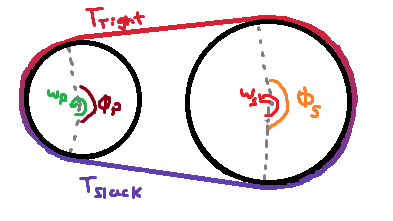
\includegraphics[width=0.9\textwidth]{./illustrations/slip/tension_slack_taught.png}
\caption{Torque transmission requires a tight--slack tension difference across the wrap.}
\label{fig:tight_slack}
\end{figure}

This tension difference arises because the pulley applies tangential
traction to the belt along the wrap angle \(\phi_j\).
The cumulative effect of this traction changes the belt tension
progressively from the slack side to the tight side.

At effective contact radius \(r_{j,\mathrm{eff}}\), the transmitted torque is

\begin{equation}
\tau_j
=
r_{j,\mathrm{eff}}\,\Delta T_j,
\qquad
|\tau_j|
=
r_{j,\mathrm{eff}}\,|\Delta T_j|.
\label{eq:tau_from_deltaT}
\end{equation}

Thus, limiting the transmitted torque is equivalent to limiting
the admissible tension difference \(\Delta T_j\).

% --------------------------------------------------------------

Under \AssRef{assump:ideal_friction} and
\AssRef{assump:constant_friction},
the belt--pulley interface obeys a Coulomb friction law with constant
coefficient \(\mu\).
The tangential traction at any point along the wrap
is therefore bounded by the local normal load:
\[
|F_f| \le \mu N.
\]

The largest admissible tension difference for a given pulley state and
transmission direction occurs when friction is fully mobilized everywhere
along the wrap, i.e.\ at impending slip.
Beyond this point, additional tension rise cannot be supported and
sliding must occur.

We therefore define a maximum supported tension difference
\(\Delta T_{j,\max}\), corresponding to the friction-saturated state,
and the associated torque capacity

\begin{equation}
\tau_{j,\max}
=
r_{j,\mathrm{eff}}\,\Delta T_{j,\max}.
\label{eq:tau_max_def}
\end{equation}

The next subsection computes \(\Delta T_{j,\max}\) by examining the
incremental change in belt tension along the wrap.

\begin{remarkbox}[Remark (Friction)]
TODO: Discuss other options for modelling friction of the rubber belt, reference that paper. Appendix?
\end{remarkbox}



\subsection{Differential Belt Element and Tangential Force Balance}
\label{sec:traction_element}

To determine the maximum admissible tension difference
$\Delta T_{j,\max}$ introduced in \Sec{sec:traction_overview},
we now examine how belt tension changes \emph{locally}
as the belt passes around a generic pulley
$j \in \{p,s\}$.

Specifically, we seek an expression for the incremental
tension change $\dd T_j$ over a differential wrap angle $\dd\theta$.
Once $\dd T_j$ is related to the available friction at the interface,
integration over the total wrap angle $\phi_j$ will yield
$\Delta T_{j,\max}$.

% --------------------------------------------------------------

\begin{figure}[H]
    \centering
    \includegraphics[width=0.55\linewidth]{./illustrations/belt_element.png}
    \caption{Free-body diagram of a differential belt element spanning $\dd \theta$.}
    \label{fig:traction_element}
\end{figure}

Consider the differential belt element shown in \Fig{fig:traction_element},
spanning an infinitesimal wrap angle $\dd\theta$ on pulley $j$.
The belt tension entering the element is $T_j$,
and leaving is $T_j + \dd T_j$.

The pulley applies to this element:
\begin{itemize}
    \item a differential normal force $\dd N_j$ (radial),
    \item a differential tangential friction force $\dd F_{f,j}$.
\end{itemize}

The positive tangential direction is taken along the midpoint tangent
of the element, consistent with increasing wrap angle and with increasing
belt tension from the slack side toward the tight side.

% --------------------------------------------------------------
\paragraph{Tangential Newton's Second Law}

Applying \theoryRef{th:newton-trans} in the tangential direction gives

\begin{equation}
\sum F_t = \dd m_j \, a_{t,j},
\label{eq:newton_tangential}
\end{equation}

where $a_{t,j}$ is the tangential acceleration of the belt material at the
contact point on pulley $j$.

The tangential components of the end tensions follow directly from geometry:

\begin{align}
(T_j)_t &= T_j\cos\!\left(\frac{\dd \theta}{2}\right),
\\[4pt]
(T_j+\dd T_j)_t &= (T_j+\dd T_j)\cos\!\left(\frac{\dd \theta}{2}\right).
\end{align}

The left-end tension acts in the positive tangential direction,
while the right-end tension acts in the negative tangential direction.
Including the differential friction force, the tangential force balance becomes

\begin{equation}
T_j\cos\!\left(\frac{\dd \theta}{2}\right)
-
(T_j+\dd T_j)\cos\!\left(\frac{\dd \theta}{2}\right)
+
\dd F_{f,j}
=
\dd m_j\,a_{t,j}.
\label{eq:tangential_balance_expanded}
\end{equation}

Simplifying the first two terms exactly gives

\begin{equation}
-\dd T_j \cos\!\left(\frac{\dd \theta}{2}\right)
+
\dd F_{f,j}
=
\dd m_j\,a_{t,j}.
\label{eq:tangential_balance_simplified}
\end{equation}

Rearranging,

\begin{equation}
\dd T_j \cos\!\left(\frac{\dd \theta}{2}\right)
=
\dd F_{f,j}
-
\dd m_j\,a_{t,j}.
\label{eq:dT_exact}
\end{equation}

% --------------------------------------------------------------
\paragraph{Belt mass element}

From \Eq{eq:dm_belt_wrap}, the belt mass associated with the differential
contact element on pulley $j$ is

\begin{equation}
\dd m_j = \rho_b A_b r_{j,\mathrm{cm}}\,\dd\theta.
\end{equation}

Thus,

\begin{equation}
\dd m_j\,a_{t,j}
=
\rho_b A_b r_{j,\mathrm{cm}} a_{t,j} \, \dd \theta.
\label{eq:dm_at}
\end{equation}

Substituting into \Eq{eq:dT_exact} gives

\begin{equation}
\dd T_j \cos\!\left(\frac{\dd \theta}{2}\right)
=
\dd F_{f,j}
-
\rho_b A_b r_{j,\mathrm{cm}} a_{t,j} \, \dd \theta.
\label{eq:dT_with_mass}
\end{equation}

% --------------------------------------------------------------
\paragraph{Friction limit and impending slip}

As established in \Sec{sec:traction_overview}, the maximum admissible
tension rise occurs when friction is fully mobilized along the wrap,
i.e.\ at impending slip.
At the differential level, this corresponds to

\begin{equation}
\dd F_{f,j} = \mu \, \dd N_j.
\label{eq:friction_saturated}
\end{equation}

Substituting \Eq{eq:friction_saturated} into
\Eq{eq:dT_with_mass} yields the maximum local
tension increase supported without sliding:

\begin{equation}
\dd T_{j,\max}
=
\frac{
\mu\, \dd N_j
-
\rho_b A_b r_{j,\mathrm{cm}} a_{t,j} \, \dd \theta
}{
\cos\!\left(\frac{\dd \theta}{2}\right)
}.
\label{eq:dT_max_local}
\end{equation}

% ==============================================================
\subsection{Integration Across the Wrap}
\label{sec:traction_wrap}

The tight--slack tension difference introduced in
\Sec{sec:traction_overview} is obtained by accumulating the
incremental tension changes \(\dd T_j\) along the contact arc of pulley
\(j \in \{p,s\}\).
Since the belt tension evolves continuously around the wrap,

\begin{equation}
\Delta T_j
=
T_{j,\mathrm{tight}} - T_{j,\mathrm{slack}}
=
\int_{-\phi_j/2}^{\phi_j/2} \dd T_j.
\label{eq:deltaT_integral_def}
\end{equation}

Accordingly, the maximum admissible tension difference is obtained
by integrating the local maximum increment \(\dd T_{j,\max}\) from
\Eq{eq:dT_max_local}:

\begin{equation}
\Delta T_{j,\max}
=
\int_{-\phi_j/2}^{\phi_j/2}
\frac{
\mu\, \dd N_j
-
\rho_b A_b r_{j,\mathrm{cm}} a_{t,j} \, \dd \theta
}{
\cos\!\left(\frac{\dd\theta}{2}\right)
}.
\label{eq:deltaT_integral}
\end{equation}

In the differential limit \(\dd\theta \to 0\),
\(\cos(\dd\theta/2) \to 1\), so this reduces to

\begin{equation}
\Delta T_{j,\max}
=
\int_{-\phi_j/2}^{\phi_j/2} \mu\, \dd N_j
-
\int_{-\phi_j/2}^{\phi_j/2}
\rho_b A_b r_{j,\mathrm{cm}} a_{t,j} \, \dd \theta.
\label{eq:deltaT_after_limit}
\end{equation}

The first integral is the total normal load carried over the wrap of
pulley \(j\), which we denote by

\begin{equation}
N_{\phi,j}
\;\equiv\;
\int_{-\phi_j/2}^{\phi_j/2} \dd N_j.
\label{eq:Nphi_def}
\end{equation}

The explicit relationship between \(N_{\phi,j}\) and the axial
clamping force is derived in \Sec{sec:normal_from_clamp}.

From \AssRef{assump:uniform_contact_radius},
\(r_{j,\mathrm{cm}}\) and \(a_{t,j}\) are uniform over the wrap,
so the second integral simplifies to
\(
\rho_b A_b r_{j,\mathrm{cm}} a_{t,j} \phi_j
\).
Hence,

\begin{equation}
\Delta T_{j,\max}
=
\mu N_{\phi,j}
-
\rho_b A_b r_{j,\mathrm{cm}} a_{t,j} \phi_j.
\label{eq:deltaT_final}
\end{equation}

Thus, the maximum admissible tension difference for pulley \(j\)
depends on two remaining quantities:
the total wrap normal load \(N_{\phi,j}\) and the tangential
belt acceleration \(a_{t,j}\).

\subsection{Tangential Acceleration of a Belt Element on a Circular Wrap}
\label{sec:belt_tangential_accel}

In \Eq{eq:deltaT_final}, Newton's second law is applied \emph{along the local
direction of belt motion}, so we require an explicit expression for the
tangential acceleration \(a_{t,j}\) of the belt material on pulley \(j\).
Since the inertial term acts on the belt element mass, the relevant kinematics
are those of the belt element centroid, located at radius
\(r_{j,\mathrm{cm}}(t)\).

\paragraph{Goal}

For a belt element of differential mass \(\dd m_j\) moving along the wrap of
pulley \(j\), the tangential force balance uses
\[
\sum F_t = \dd m_j\,a_{t,j}.
\]
Our goal is therefore to compute \(a_{t,j}\) from the belt kinematics when both
the local angular speed and the centroid radius may vary:
\[
\omega_j(t)=\dot\theta_j(t),
\qquad
\dot\omega_j(t),
\qquad
r_{j,\mathrm{cm}}(t),
\qquad
\dot r_{j,\mathrm{cm}}(t).
\]

\paragraph{Coordinate system and unit vectors}

Because we care about forces \emph{along the belt}, we choose a basis aligned
with the local wrap geometry on pulley \(j\):
\begin{itemize}
    \item \(\mathbf e_{r,j}(t)\) points radially outward from the pulley center
    to the belt point,
    \item \(\mathbf e_{\theta,j}(t)\) is the unit tangent, obtained by rotating
    \(\mathbf e_{r,j}\) by \(+90^\circ\) in the direction of increasing
    \(\theta_j\).
\end{itemize}

The tangential direction of belt motion is therefore exactly
\(\mathbf e_{\theta,j}\).

\begin{figure}[H]
    \centering
    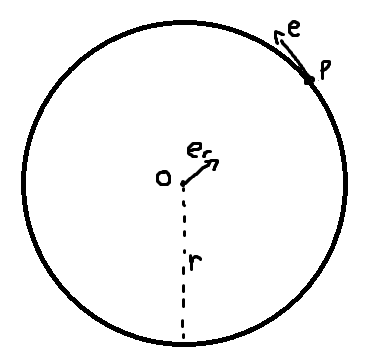
\includegraphics[width=0.7\textwidth]{./illustrations/slip/polar.png}
    \caption{Definition of the radial and tangential unit vectors.}
    \label{fig:polar_basis_placeholder}
\end{figure}

\paragraph{Tangential acceleration as a component of \(\mathbf a\)}

Tangential acceleration is the component of the acceleration vector along
\(\mathbf e_{\theta,j}\):
\begin{equation}
a_{t,j} \equiv \mathbf a_j\cdot \mathbf e_{\theta,j}.
\label{eq:at_component_def}
\end{equation}

We therefore compute the full acceleration \(\mathbf a_j=\dot{\mathbf v}_j\)
and then read off its \(\mathbf e_{\theta,j}\) component.

\paragraph{Step 1: position and velocity}

The position of the belt element centroid relative to the pulley center is
\begin{equation}
\mathbf r_j(t) = r_{j,\mathrm{cm}}(t)\,\mathbf e_{r,j}(t).
\label{eq:position_polar}
\end{equation}

Differentiating \Eq{eq:position_polar} gives
\begin{equation}
\mathbf v_j = \dot{\mathbf r}_j
= \dot r_{j,\mathrm{cm}}\,\mathbf e_{r,j}
+ r_{j,\mathrm{cm}}\,\dot{\mathbf e}_{r,j}.
\label{eq:velocity_before_unit_rates}
\end{equation}

Thus, even if \(r_{j,\mathrm{cm}}\) were constant, the velocity would still
depend on the rotation of the local basis.

\paragraph{Step 2: time derivatives of the unit vectors}

Over a small angular change \(\dd\theta_j\), the unit vectors rotate rigidly by
the same angle. Hence
\begin{equation}
\frac{\dd \mathbf e_{r,j}}{\dd\theta_j} = \mathbf e_{\theta,j},
\qquad
\frac{\dd \mathbf e_{\theta,j}}{\dd\theta_j} = -\mathbf e_{r,j}.
\label{eq:unit_vectors_angle_derivatives}
\end{equation}

Using the chain rule with
\(
\omega_j=\dot\theta_j
\),
these become
\begin{equation}
\dot{\mathbf e}_{r,j} = \omega_j\,\mathbf e_{\theta,j},
\qquad
\dot{\mathbf e}_{\theta,j} = -\omega_j\,\mathbf e_{r,j}.
\label{eq:unit_vectors_time_derivatives}
\end{equation}

\paragraph{Step 3: velocity in radial--tangential form}

Substituting \Eq{eq:unit_vectors_time_derivatives} into
\Eq{eq:velocity_before_unit_rates} gives
\begin{equation}
\mathbf v_j
=
\dot r_{j,\mathrm{cm}}\,\mathbf e_{r,j}
+
r_{j,\mathrm{cm}}\omega_j\,\mathbf e_{\theta,j}.
\label{eq:velocity_polar}
\end{equation}

Thus, \(\dot r_{j,\mathrm{cm}}\) is the radial speed and
\(r_{j,\mathrm{cm}}\omega_j\) is the tangential speed.

\paragraph{Step 4: acceleration and tangential component}

Differentiating \Eq{eq:velocity_polar} gives
\begin{align}
\mathbf a_j = \dot{\mathbf v}_j
&=
\frac{\dd}{\dd t}\big(\dot r_{j,\mathrm{cm}}\,\mathbf e_{r,j}\big)
+
\frac{\dd}{\dd t}\big(r_{j,\mathrm{cm}}\omega_j\,\mathbf e_{\theta,j}\big)
\nonumber\\[6pt]
&=
\ddot r_{j,\mathrm{cm}}\,\mathbf e_{r,j}
+
\dot r_{j,\mathrm{cm}}\,\dot{\mathbf e}_{r,j}
+
(\dot r_{j,\mathrm{cm}}\,\omega_j + r_{j,\mathrm{cm}}\,\dot\omega_j)\mathbf e_{\theta,j}
+
r_{j,\mathrm{cm}}\omega_j\,\dot{\mathbf e}_{\theta,j}.
\label{eq:accel_expand}
\end{align}

Substituting the unit-vector derivatives from
\Eq{eq:unit_vectors_time_derivatives} and collecting like terms yields
\begin{align}
\mathbf a_j
&=
\ddot r_{j,\mathrm{cm}}\,\mathbf e_{r,j}
+
\dot r_{j,\mathrm{cm}}(\omega_j\,\mathbf e_{\theta,j})
+
(\dot r_{j,\mathrm{cm}}\,\omega_j + r_{j,\mathrm{cm}}\,\dot\omega_j)\mathbf e_{\theta,j}
+
r_{j,\mathrm{cm}}\omega_j(-\omega_j\,\mathbf e_{r,j})
\nonumber\\[6pt]
&=
\big(\ddot r_{j,\mathrm{cm}} - r_{j,\mathrm{cm}}\omega_j^2\big)\mathbf e_{r,j}
+
\big(r_{j,\mathrm{cm}}\dot\omega_j + 2\dot r_{j,\mathrm{cm}}\,\omega_j\big)\mathbf e_{\theta,j}.
\label{eq:accel_polar}
\end{align}

By \Eq{eq:at_component_def}, the tangential acceleration is therefore
\begin{equation}
a_{t,j}
=
r_{j,\mathrm{cm}}\dot\omega_j + 2\dot r_{j,\mathrm{cm}}\,\omega_j.
\label{eq:at_final}
\end{equation}

\paragraph{Origin of the factor of 2}

The two \(\dot r_{j,\mathrm{cm}}\,\omega_j\) contributions in
\Eq{eq:accel_polar} arise from two distinct effects:
\begin{itemize}
    \item \(\dot r_{j,\mathrm{cm}}\,\dot{\mathbf e}_{r,j}\): the radial velocity
    \(\dot r_{j,\mathrm{cm}}\,\mathbf e_{r,j}\) acquires a tangential contribution because
    the radial direction itself rotates at rate \(\omega_j\),
    \item \(\frac{\dd}{\dd t}(r_{j,\mathrm{cm}}\omega_j)\): the tangential speed changes when
    the centroid radius changes.
\end{itemize}

Together, these give the total term \(2\dot r_{j,\mathrm{cm}}\,\omega_j\).
\subsection{Normal Force from Axial Clamping}
\label{sec:normal_from_clamp}

The traction bound \Eq{eq:deltaT_final} depends on the total normal load
over the wrap of pulley \(j\),
\[
N_{\phi,j} \equiv \int_{-\phi_j/2}^{\phi_j/2} \dd N_j.
\]
We now express \(N_{\phi,j}\) in terms of the axial clamping force
generated by that pulley.

% --------------------------------------------------------------
\paragraph{Axial clamp produces radial normal load}

The belt is pressed between two opposing conical sheaves.
On pulley \(j\), an axial clamping force \(F_{\mathrm{ax},j}\) pushes the
sheaves together.
Because the sheave faces are inclined at cone half-angle \(\beta\),
this axial force generates a radial normal load on the belt.

From the conical geometry relation established in
\Eq{eq:cone_geometry_diff},

\[
\frac{\dd r_j}{\dd s} = \frac{1}{2\tan\beta}.
\]

To relate the axial and radial forces consistently, we use virtual work.
The incremental work done by the axial clamp must equal the incremental
work associated with radial compression of the belt:

\[
F_{\mathrm{ax},j}\,\dd s
=
F_{\mathrm{rad},j}\,\dd r_j.
\]

Substituting
\(
\dd r_j = \left(\dd r_j/\dd s\right)\dd s
\)
gives

\begin{equation}
F_{\mathrm{rad},j}
=
\frac{F_{\mathrm{ax},j}}{\dd r_j/\dd s}
=
2F_{\mathrm{ax},j}\tan\beta.
\label{eq:Frad_from_Fax}
\end{equation}

Thus, the axial clamp force on pulley \(j\) produces a total radial normal load

\begin{equation}
F_{\mathrm{rad},j} = 2F_{\mathrm{ax},j}\tan\beta.
\label{eq:Frad_simple}
\end{equation}

% --------------------------------------------------------------
\paragraph{Identification with the wrap-normal load}

The radial load \(F_{\mathrm{rad},j}\) derived above represents the total inward
force applied by the two sheave faces of pulley \(j\) onto the belt.
That load is carried by the distributed belt--pulley contact forces
\(\dd N_j\) along the wrap.

Therefore, the total normal load available for traction on pulley \(j\) is

\begin{equation}
\boxed{
N_{\phi,j} = F_{\mathrm{rad},j} = 2F_{\mathrm{ax},j}\tan\beta.
}
\label{eq:Nphi_from_Fax}
\end{equation}

This result states that the total wrap normal load, and hence the normal
load available for traction, is set directly by the axial clamping force
through the cone geometry.

\subsection{Torque Capacity}
\label{sec:tau_capacity}

From \Sec{sec:traction_overview}, the maximum transmissible torque on pulley
\(j\) is determined by the maximum admissible tension difference across the
wrap:
\begin{equation}
\tau_{j,\max}
=
r_{j,\mathrm{eff}}\,\Delta T_{j,\max}.
\label{eq:tau_max_repeat}
\end{equation}

Using the integrated result from \Eq{eq:deltaT_final},
together with the wrap-normal relation \Eq{eq:Nphi_from_Fax} and the
belt tangential acceleration from \Eq{eq:at_final},
\[
\Delta T_{j,\max}
=
\mu N_{\phi,j}
-
\rho_b A_b r_{j,\mathrm{cm}} a_{t,j} \phi_j,
\qquad
N_{\phi,j} = 2F_{\mathrm{ax},j}\tan\beta,
\qquad
a_{t,j}
=
r_{j,\mathrm{cm}}\dot{\omega}_j
+
2\dot r_{j,\mathrm{cm}}\,\omega_j,
\]
the explicit torque-capacity expression becomes

\bigeq{eq:tau_capacity_final}{Pulley Torque Capacity}{
\tau_{j,\max}
=
r_{j,\mathrm{eff}}
\left[
2\mu F_{\mathrm{ax},j}\tan\beta
-
\rho_b A_b r_{j,\mathrm{cm}} \phi_j
\left(
r_{j,\mathrm{cm}}\dot{\omega}_j
+
2\dot r_{j,\mathrm{cm}}\,\omega_j
\right)
\right].
}

The remaining task is to substitute the appropriate rotational acceleration
\(\dot{\omega}_j\) and axial clamp force \(F_{\mathrm{ax},j}\) for each pulley 
to obtain explicit bounds on the coupling torque.

% --------------------------------------------------------------
\begin{remarkbox}[Remark (Why this differs from the classical capstan exponential)]
In the classical capstan problem, the normal load is generated \emph{by the belt tension}
itself (a larger tension implies a proportionally larger contact normal),
which leads to the exponential relation $T_1/T_2 = e^{\mu\phi}$.

Here, the normal load is imposed externally by the clamping mechanism:
$N_\phi$ is determined by $F_{\mathrm{ax}}$ through \Eq{eq:Nphi_from_Fax}.
Therefore, the available traction scales \emph{linearly} with clamping force,
not exponentially with belt tension.
Centrifugal loading and ratio change enter additionally through the inertial term
in \Eq{eq:tau_capacity_final}.
\end{remarkbox}

% --------------------------------------------------------------
\begin{remarkbox}[Remark (Torque-Reactive Clamping and Implicit Capacity at the Secondary)]
For the secondary pulley, the specific axial clamp force
$F_{\mathrm{ax}}$ used in this model depends on the transmitted torque
$\tau_s$ (see \Eq{eq:secondary_axial}).  
However, the traction capacity $\tau_{\max}$ derived above depends
on $F_{\mathrm{ax}}$ through \Eq{eq:Nphi_from_Fax} and
\Eq{eq:tau_capacity_final}.  

Consequently, at the secondary interface the admissible torque
satisfies an implicit relation of the form
\[
|\tau_s| \le \tau_{\max}\big(F_{\mathrm{ax}}(\tau_s)\big).
\]

In other words, the transmitted torque influences the clamp force,
the clamp force determines the traction capacity,
and that capacity bounds the transmitted torque.
This circular dependence arises only because the secondary
mechanism is torque-reactive.

For the specific secondary model adopted in this work,
this implicit inequality can be reduced to a closed-form solution
(see Appendix~\ref{sec:appendix-secondary-capacity-closure}).
The explicit algebra is omitted here to preserve clarity,
as it depends on the detailed functional form of
$F_{\mathrm{ax}}(s,\tau_s)$ and is not required
to understand the main traction derivation.
\end{remarkbox}


% --------------------------------------------------------------
\subsection{Section Conclusion and Transition}
\label{sec:traction_conclusion}

This section derived a traction-limited torque bound for a single pulley.

Equation \Eq{eq:tau_capacity_final} gives the maximum torque
that can be transmitted at the current operating state.
It depends only on:

\begin{itemize}
    \item axial clamping force $F_{\mathrm{ax}}$,
    \item cone angle $\beta$,
    \item wrap angle $\phi$,
    \item belt mass and kinematics.
\end{itemize}

No exponential amplification occurs because the normal force
is externally imposed and bounded.

% ==============================================================


\section{Pulley-Specific Traction Bounds and Coupling Torque Closure}
\label{sec:pulley_specific_bounds}

The generic capacity law \Eq{eq:tau_capacity_final} gives the maximum
transmissible torque for a pulley \(j\) in terms of its local clamping force,
geometry, and belt kinematics.
To obtain usable limits on the coupling torque, this expression must now be
specialized to the primary and secondary pulleys.

For each pulley, the procedure is the same:

\begin{enumerate}
    \item identify the torque transmitted at that pulley,
    \item substitute the appropriate rotational acceleration,
    \item substitute the pulley-specific axial clamping-force model,
    \item solve the resulting implicit inequality for the admissible torque range.
\end{enumerate}

On the primary side this is relatively direct, since the axial clamp force does
not depend explicitly on the transmitted torque.
On the secondary side, the torque-reactive helix introduces an additional
dependence on transmitted torque, so the algebra is more involved.

The resulting admissible interval for the coupling torque is obtained by
intersecting the bounds contributed by the two pulleys.

% --------------------------------------------------------------
\subsection{Primary Pulley Traction Bounds}
\label{sec:primary_tau_limits}

On the primary pulley, the transmitted torque at the belt contact is the
coupling torque itself.
Thus, applying \Eq{eq:tau_capacity_final} with \(j=p\) gives

\begin{equation}
\tau_{p,\max}
=
r_{p,\mathrm{eff}}
\left[
2\mu F_{\mathrm{ax},p}\tan\beta
-
\rho_b A_b r_{p,\mathrm{cm}} \phi_p
\left(
r_{p,\mathrm{cm}}\dot{\omega}_p
+
2\dot r_{p,\mathrm{cm}}\,\omega_p
\right)
\right].
\label{eq:tau_p_max_generic}
\end{equation}

Therefore, admissible transmission at the primary requires
\begin{equation}
|\tau_c| \le \tau_{p,\max}.
\label{eq:tau_p_capacity_start}
\end{equation}

From the primary rotational dynamics \Eq{eq:primary_rot_dyn},
\begin{equation}
\dot{\omega}_p
=
\frac{\tau_{\mathrm{eng}}-\tau_c}{I_p}.
\label{eq:omega_dot_p_from_eom}
\end{equation}

Substituting \Eq{eq:omega_dot_p_from_eom} into \Eq{eq:tau_p_max_generic} gives
\begin{equation}
|\tau_c|
\le
r_{p,\mathrm{eff}}
\left[
2\mu F_{\mathrm{ax},p}\tan\beta
-
\rho_b A_b r_{p,\mathrm{cm}} \phi_p
\left(
r_{p,\mathrm{cm}}\frac{\tau_{\mathrm{eng}}-\tau_c}{I_p}
+
2\dot r_{p,\mathrm{cm}}\,\omega_p
\right)
\right].
\label{eq:tau_p_capacity_implicit}
\end{equation}

Since \(\tau_c\) appears on both sides, the positive and negative directions
must be treated separately.

\paragraph{Positive-direction bound \(\tau_c \ge 0\)}

For \(\tau_c \ge 0\), \(|\tau_c|=\tau_c\), so
\begin{align}
\tau_c
&\le
r_{p,\mathrm{eff}}
\left[
2\mu F_{\mathrm{ax},p}\tan\beta
-
\rho_b A_b r_{p,\mathrm{cm}} \phi_p
\left(
r_{p,\mathrm{cm}}\frac{\tau_{\mathrm{eng}}-\tau_c}{I_p}
+
2\dot r_{p,\mathrm{cm}}\,\omega_p
\right)
\right]
\nonumber\\[4pt]
\frac{\tau_c}{r_{p,\mathrm{eff}}}
-
\rho_b A_b r_{p,\mathrm{cm}} \phi_p
\frac{r_{p,\mathrm{cm}}}{I_p}\tau_c
&\le
2\mu F_{\mathrm{ax},p}\tan\beta
-
\rho_b A_b r_{p,\mathrm{cm}} \phi_p
\left(
\frac{r_{p,\mathrm{cm}}}{I_p}\tau_{\mathrm{eng}}
+
2\dot r_{p,\mathrm{cm}}\,\omega_p
\right).
\label{eq:tau_p_plus_rearrange}
\end{align}

Hence,
\begin{equation}
\tau_c \le \tau_{p,+},
\qquad
\tau_{p,+}
=
\frac{
2\mu F_{\mathrm{ax},p}\tan\beta
-
\rho_b A_b r_{p,\mathrm{cm}} \phi_p
\left(
\dfrac{r_{p,\mathrm{cm}}}{I_p}\tau_{\mathrm{eng}}
+
2\dot r_{p,\mathrm{cm}}\,\omega_p
\right)
}{
\dfrac{1}{r_{p,\mathrm{eff}}}
-
\rho_b A_b r_{p,\mathrm{cm}} \phi_p
\dfrac{r_{p,\mathrm{cm}}}{I_p}
}.
\label{eq:tau_p_plus}
\end{equation}

\paragraph{Negative-direction bound \(\tau_c \le 0\)}

For \(\tau_c \le 0\), \(|\tau_c|=-\tau_c\), so
\begin{align}
-\tau_c
&\le
r_{p,\mathrm{eff}}
\left[
2\mu F_{\mathrm{ax},p}\tan\beta
-
\rho_b A_b r_{p,\mathrm{cm}} \phi_p
\left(
r_{p,\mathrm{cm}}\frac{\tau_{\mathrm{eng}}-\tau_c}{I_p}
+
2\dot r_{p,\mathrm{cm}}\,\omega_p
\right)
\right]
\nonumber\\[4pt]
-\frac{\tau_c}{r_{p,\mathrm{eff}}}
-
\rho_b A_b r_{p,\mathrm{cm}} \phi_p
\frac{r_{p,\mathrm{cm}}}{I_p}\tau_c
&\le
2\mu F_{\mathrm{ax},p}\tan\beta
-
\rho_b A_b r_{p,\mathrm{cm}} \phi_p
\left(
\frac{r_{p,\mathrm{cm}}}{I_p}\tau_{\mathrm{eng}}
+
2\dot r_{p,\mathrm{cm}}\,\omega_p
\right).
\label{eq:tau_p_minus_rearrange}
\end{align}

Hence,
\begin{equation}
\tau_c \ge \tau_{p,-},
\qquad
\tau_{p,-}
=
-\frac{
2\mu F_{\mathrm{ax},p}\tan\beta
-
\rho_b A_b r_{p,\mathrm{cm}} \phi_p
\left(
\dfrac{r_{p,\mathrm{cm}}}{I_p}\tau_{\mathrm{eng}}
+
2\dot r_{p,\mathrm{cm}}\,\omega_p
\right)
}{
\dfrac{1}{r_{p,\mathrm{eff}}}
+
\rho_b A_b r_{p,\mathrm{cm}} \phi_p
\dfrac{r_{p,\mathrm{cm}}}{I_p}
}.
\label{eq:tau_p_minus}
\end{equation}

Therefore, the primary pulley contributes the admissible interval
\begin{equation}
\boxed{
\tau_{p,-} \le \tau_c \le \tau_{p,+}.
}
\label{eq:primary_tau_interval}
\end{equation}

Finally, substituting the primary axial-force model
\Eq{eq:primary_axial}
into \Eq{eq:tau_p_plus} and \Eq{eq:tau_p_minus}, with
\[
F_{\mathrm{ax},p}
=
m_f\omega_p^2\,r_f(s)\,\frac{\dd r_f}{\dd s}
-
k_p\bigl(x_{p,0}+s\bigr),
\]
gives the explicit primary traction bounds

\bigeq{eq:tau_p_plus_expanded}{Primary Traction Upper Bound}{
\tau_{p,+}
=
\frac{
2\mu\tan\beta
\left[
m_f\omega_p^2\,r_f(s)\,\dfrac{\dd r_f}{\dd s}
-
k_p\bigl(x_{p,0}+s\bigr)
\right]
-
\rho_b A_b r_{p,\mathrm{cm}} \phi_p
\left(
\dfrac{r_{p,\mathrm{cm}}}{I_p}\tau_{\mathrm{eng}}
+
2\dot r_{p,\mathrm{cm}}\,\omega_p
\right)
}{
\dfrac{1}{r_{p,\mathrm{eff}}}
-
\rho_b A_b r_{p,\mathrm{cm}} \phi_p
\dfrac{r_{p,\mathrm{cm}}}{I_p}
},
}

and

\bigeq{eq:tau_p_minus_expanded}{Primary Traction Lower Bound}{
\tau_{p,-}
=
-\frac{
2\mu\tan\beta
\left[
m_f\omega_p^2\,r_f(s)\,\dfrac{\dd r_f}{\dd s}
-
k_p\bigl(x_{p,0}+s\bigr)
\right]
-
\rho_b A_b r_{p,\mathrm{cm}} \phi_p
\left(
\dfrac{r_{p,\mathrm{cm}}}{I_p}\tau_{\mathrm{eng}}
+
2\dot r_{p,\mathrm{cm}}\,\omega_p
\right)
}{
\dfrac{1}{r_{p,\mathrm{eff}}}
+
\rho_b A_b r_{p,\mathrm{cm}} \phi_p
\dfrac{r_{p,\mathrm{cm}}}{I_p}
}.
}

% --------------------------------------------------------------
\subsection{Secondary Pulley Traction Bounds}
\label{sec:secondary_tau_limits}

On the secondary pulley, the transmitted torque at the belt contact is
\(\tau_s\).
Applying \Eq{eq:tau_capacity_final} with \(j=s\) therefore gives

\begin{equation}
\tau_{s,\max}
=
r_{s,\mathrm{eff}}
\left[
2\mu F_{\mathrm{ax},s}\tan\beta
-
\rho_b A_b r_{s,\mathrm{cm}} \phi_s
\left(
r_{s,\mathrm{cm}}\dot{\omega}_s
+
2\dot r_{s,\mathrm{cm}}\,\omega_s
\right)
\right].
\label{eq:tau_s_max_generic}
\end{equation}

Accordingly, admissible transmission at the secondary requires
\begin{equation}
|\tau_s| \le \tau_{s,\max}.
\label{eq:tau_s_capacity_start}
\end{equation}

From the secondary rotational dynamics \Eq{eq:secondary_rot_dyn},
\begin{equation}
\dot{\omega}_s
=
\frac{\tau_s-\tau_{\mathrm{load}}}{I_s}.
\label{eq:omega_dot_s_from_eom}
\end{equation}

From the secondary axial-force model \Eq{eq:secondary_axial},
\begin{equation}
F_{\mathrm{ax},s}(s,\tau_s)
=
\frac{
\tau_s + k_{s,\theta}\!\bigl(\theta_{s,0}+\theta_s(s)\bigr)
}{2}
\frac{\dd \theta_s}{\dd s}
+
k_{s,x}(x_{s,0}-s).
\label{eq:Fax_s_sub}
\end{equation}

Substituting \Eq{eq:omega_dot_s_from_eom} and \Eq{eq:Fax_s_sub} into
\Eq{eq:tau_s_max_generic} gives the implicit secondary traction inequality

\begin{equation}
\begin{aligned}
|\tau_s|
\le\;&
r_{s,\mathrm{eff}}
\Biggl[
2\mu\tan\beta
\left(
\frac{
\tau_s + k_{s,\theta}\!\bigl(\theta_{s,0}+\theta_s(s)\bigr)
}{2}
\frac{\dd \theta_s}{\dd s}
+
k_{s,x}(x_{s,0}-s)
\right)
\\
&\qquad
-
\rho_b A_b r_{s,\mathrm{cm}} \phi_s
\left(
r_{s,\mathrm{cm}}\frac{\tau_s-\tau_{\mathrm{load}}}{I_s}
+
2\dot r_{s,\mathrm{cm}}\,\omega_s
\right)
\Biggr].
\end{aligned}
\label{eq:tau_s_capacity_implicit}
\end{equation}

Since \(\tau_s\) appears both through the acceleration term and through the
torque-reactive axial clamping force, the positive and negative transmission
directions must again be treated separately.

\paragraph{Positive-direction bound \(\tau_s \ge 0\)}

For \(\tau_s \ge 0\), \(|\tau_s|=\tau_s\).
Collecting the \(\tau_s\) terms on the left gives
\begin{align}
\frac{\tau_s}{r_{s,\mathrm{eff}}}
-
\mu\tan\beta \frac{\dd\theta_s}{\dd s}\,\tau_s
\rho_b A_b r_{s,\mathrm{cm}} \phi_s
\frac{r_{s,\mathrm{cm}}}{I_s}\,\tau_s
\;\le\;&
\mu\tan\beta
\frac{\dd\theta_s}{\dd s}
k_{s,\theta}\!\bigl(\theta_{s,0}+\theta_s(s)\bigr)
\nonumber\\
&+
2\mu\tan\beta\,k_{s,x}(x_{s,0}-s)
\nonumber\\
&+
\rho_b A_b r_{s,\mathrm{cm}} \phi_s
\left(
\frac{r_{s,\mathrm{cm}}}{I_s}\tau_{\mathrm{load}}
-
2\dot r_{s,\mathrm{cm}}\,\omega_s
\right).
\label{eq:tau_s_plus_rearrange}
\end{align}

Hence,
\begin{equation}
\tau_s \le \tau_{s,+},
\label{eq:tau_s_plus_ineq}
\end{equation}
with
\bigeq{eq:tau_s_plus}{Secondary Positive Traction Limit}{
\tau_{s,+}
=
\frac{
\mu\tan\beta
\left[
\frac{\dd\theta_s}{\dd s}\,
k_{s,\theta}\!\bigl(\theta_{s,0}+\theta_s(s)\bigr)
+
2k_{s,x}(x_{s,0}-s)
\right]
+
\rho_b A_b r_{s,\mathrm{cm}} \phi_s
\left(
\frac{r_{s,\mathrm{cm}}}{I_s}\tau_{\mathrm{load}}
-
2\dot r_{s,\mathrm{cm}}\,\omega_s
\right)
}{
\frac{1}{r_{s,\mathrm{eff}}}
-
\mu\tan\beta \frac{\dd\theta_s}{\dd s}
+
\rho_b A_b r_{s,\mathrm{cm}} \phi_s
\frac{r_{s,\mathrm{cm}}}{I_s}
}.
}

\paragraph{Negative-direction bound \(\tau_s \le 0\)}

For \(\tau_s \le 0\), \(|\tau_s|=-\tau_s\).
Collecting the \(\tau_s\) terms on the left gives
\begin{align}
-\frac{\tau_s}{r_{s,\mathrm{eff}}}
-
\mu\tan\beta \frac{\dd\theta_s}{\dd s}\,\tau_s
+
\rho_b A_b r_{s,\mathrm{cm}} \phi_s
\frac{r_{s,\mathrm{cm}}}{I_s}\,\tau_s
\;\le\;&
\mu\tan\beta
\frac{\dd\theta_s}{\dd s}
k_{s,\theta}\!\bigl(\theta_{s,0}+\theta_s(s)\bigr)
\nonumber\\
&+
2\mu\tan\beta\,k_{s,x}(x_{s,0}-s)
\nonumber\\
&+
\rho_b A_b r_{s,\mathrm{cm}} \phi_s
\left(
\frac{r_{s,\mathrm{cm}}}{I_s}\tau_{\mathrm{load}}
-
2\dot r_{s,\mathrm{cm}}\,\omega_s
\right).
\label{eq:tau_s_minus_rearrange}
\end{align}

Hence,
\begin{equation}
\tau_s \ge \tau_{s,-},
\label{eq:tau_s_minus_ineq}
\end{equation}
with
\bigeq{eq:tau_s_minus}{Secondary Negative Traction Limit}{
\tau_{s,-}
=
-\frac{
\mu\tan\beta
\left[
\frac{\dd\theta_s}{\dd s}\,
k_{s,\theta}\!\bigl(\theta_{s,0}+\theta_s(s)\bigr)
+
2k_{s,x}(x_{s,0}-s)
\right]
+
\rho_b A_b r_{s,\mathrm{cm}} \phi_s
\left(
\frac{r_{s,\mathrm{cm}}}{I_s}\tau_{\mathrm{load}}
-
2\dot r_{s,\mathrm{cm}}\,\omega_s
\right)
}{
\frac{1}{r_{s,\mathrm{eff}}}
+
\mu\tan\beta \frac{\dd\theta_s}{\dd s}
-
\rho_b A_b r_{s,\mathrm{cm}} \phi_s
\frac{r_{s,\mathrm{cm}}}{I_s}
}.
}

Therefore, the secondary pulley contributes the admissible interval
\begin{equation}
\boxed{
\tau_{s,-} \le \tau_s \le \tau_{s,+}.
}
\label{eq:secondary_tau_interval}
\end{equation}

\subsection{Combined Traction-Limited Coupling Law}
\label{sec:final_coupling_law}

The previous two subsections produced admissible traction intervals for each
pulley separately:
\[
\tau_{p,-} \le \tau_c \le \tau_{p,+},
\qquad
\tau_{s,-} \le \tau_s \le \tau_{s,+}.
\]

Since the transmitted state must satisfy the traction limits at
\emph{both} pulleys simultaneously, the final admissible range is obtained by
intersecting these two constraints.

Using the torque mapping
\[
\tau_s = R\,\tau_c,
\]
the secondary bounds may be written in terms of the coupling torque as
\[
\frac{\tau_{s,-}}{R}
\le
\tau_c
\le
\frac{\tau_{s,+}}{R}.
\]

Therefore, the overall admissible coupling-torque interval is

\begin{equation}
\tau_- \le \tau_c \le \tau_+,
\label{eq:tau_global_interval}
\end{equation}

with
\begin{equation}
\tau_-
=
\max\!\left(
\tau_{p,-},
\frac{\tau_{s,-}}{R}
\right),
\qquad
\tau_+
=
\min\!\left(
\tau_{p,+},
\frac{\tau_{s,+}}{R}
\right).
\label{eq:tau_pm_final}
\end{equation}

These are the final negative- and positive-direction traction limits used in
the regime law.

% --------------------------------------------------------------
\paragraph{Stick and slip regimes}

As established in \Sec{sec:transmission_regimes}, the no-slip branch is
admissible only when two conditions hold simultaneously:

\begin{enumerate}
    \item the no-slip torque lies within the admissible interval, and
    \item the relative slip metric satisfies \(v_{\Delta}=0\).
\end{enumerate}

If both conditions are satisfied, the transmission remains in stick and the
coupling torque is the no-slip torque \(\tau_{\mathrm{ns}}\).

If instead the no-slip torque lies outside the admissible interval, or if a
nonzero slip mismatch is already present, then the transmission is on a
traction-limited slip branch.
The active slip branch is selected by the sign of \(v_{\Delta}\), as introduced
in \Sec{sec:transmission_regimes}.

This gives the final coupling law

\bigeq{eq:tau_c_final}{Traction-Limited Coupling Torque Law}{
\tau_c =
\begin{cases}
\tau_{\mathrm{ns}},
&
v_{\Delta}=0
\;\text{and}\;
\tau_- \le \tau_{\mathrm{ns}} \le \tau_+,
\\[10pt]
\tau_+,
&
v_{\Delta}>0
\;\text{or}\;
\bigl(v_{\Delta}=0 \text{ and } \tau_{\mathrm{ns}}>\tau_+\bigr),
\\[10pt]
\tau_-,
&
v_{\Delta}<0
\;\text{or}\;
\bigl(v_{\Delta}=0 \text{ and } \tau_{\mathrm{ns}}<\tau_-\bigr).
\end{cases}
}


\paragraph{Interpretation}

The logic of \Eq{eq:tau_c_final} is as follows:

\begin{itemize}
    \item If the sticking solution is both kinematically compatible
    (\(v_{\Delta}=0\)) and traction-admissible
    (\(\tau_- \le \tau_{\mathrm{ns}} \le \tau_+\)),
    then the transmission remains on the no-slip branch.

    \item If the demanded no-slip torque exceeds the positive traction limit,
    the contact saturates on the positive slip branch.

    \item If the demanded no-slip torque falls below the negative traction
    limit, the contact saturates on the negative slip branch.

    \item Once slip is present, the transmission remains on the corresponding
    slip branch until the mismatch \(v_{\Delta}\) is driven back to zero.
\end{itemize}

\Eq{eq:tau_c_final} therefore closes the coupling-torque model across
both stick and slip regimes.

% ==============================================================
\section{Complete CVT Dynamic Model}
\label{sec:complete_model}

This section gathers the results of the previous derivations into one closed
nonlinear dynamical model.
No new physics is introduced here.
The goal is simply to summarize, in one place,

\begin{enumerate}
    \item the chosen state variables,
    \item the algebraic quantities computed from those states,
    \item the stick--slip torque closure,
    \item and the final governing ODEs.
\end{enumerate}

% --------------------------------------------------------------
\subsection{State Definition}

The state vector is
\begin{equation}
\mathbf{x}
=
\big(
\omega_p,\;
\omega_s,\;
s,\;
\dot s
\big),
\label{eq:state_vector}
\end{equation}
where
\begin{itemize}
    \item \(\omega_p\) is the primary pulley angular velocity,
    \item \(\omega_s\) is the secondary pulley angular velocity,
    \item \(s\) is the axial shift coordinate,
    \item \(\dot s\) is the axial shift velocity.
\end{itemize}

% --------------------------------------------------------------
\subsection{Geometry and Ratio Closure}

At each instant, the shift coordinate \(s\) determines the pulley geometry
through the belt-length constraint and the conical kinematic relations derived
earlier.
In particular, the effective radii and wrap angles are functions of \(s\), and
the geometric CVT ratio is
\begin{equation}
R(s)
=
\frac{r_{s,\mathrm{eff}}(s)}{r_{p,\mathrm{eff}}(s)}.
\label{eq:R_of_s}
\end{equation}

Its time derivative is
\begin{equation}
\dot R = \dot R(s,\dot s),
\label{eq:Rdot_of_states}
\end{equation}
as given by \Eq{eq:Rdot_final}.

Thus, once \((s,\dot s)\) are known, the model can evaluate
\[
r_{p,\mathrm{eff}},\quad
r_{s,\mathrm{eff}},\quad
r_{p,\mathrm{cm}},\quad
r_{s,\mathrm{cm}},\quad
\phi_p,\quad
\phi_s,\quad
R,\quad
\dot R,
\]
together with any other geometry-dependent terms appearing in the force and
traction models.

% --------------------------------------------------------------
\subsection{Torque Closure}

The internal torque transmitted through the CVT is the coupling torque
\(\tau_c\).
This is the central algebraic unknown of the transmission model.

\paragraph{No-slip torque demand.}

If sticking is maintained, the required coupling torque is the no-slip torque
derived in \Eq{eq:tau_ns_final}:
\begin{equation}
\tau_{\mathrm{ns}}
=
\frac{
\tau_{\mathrm{eng}}
+
\dfrac{I_p}{I_s}R\,\tau_{\mathrm{load}}
-
I_p\,\omega_s\,\dot R
}{
1+\dfrac{I_p}{I_s}R^2
}.
\label{eq:tau_ns_def_complete}
\end{equation}

\paragraph{Traction bounds.}

The pulley-specific traction limits derived in
\Sec{sec:primary_tau_limits} and \Sec{sec:secondary_tau_limits}
combine to give the final admissible interval
\begin{equation}
\tau_- \le \tau_c \le \tau_+,
\label{eq:tau_pm_complete}
\end{equation}
with
\begin{equation}
\tau_-
=
\max\!\left(
\tau_{p,-},
\frac{\tau_{s,-}}{R}
\right),
\qquad
\tau_+
=
\min\!\left(
\tau_{p,+},
\frac{\tau_{s,+}}{R}
\right),
\label{eq:tau_pm_complete_explicit}
\end{equation}
as given by \Eq{eq:tau_pm_final}.

\paragraph{Slip metric and regime selection.}

The slip metric from \Eq{eq:v_delta_def} is
\begin{equation}
v_{\Delta}
=
r_{p,\mathrm{eff}}\,\omega_p
-
r_{s,\mathrm{eff}}\,\omega_s.
\label{eq:v_delta_complete}
\end{equation}

Using \(\tau_{\mathrm{ns}}\), \(\tau_-\), \(\tau_+\), and \(v_\Delta\), the
actual coupling torque is selected by the stick--slip law
\Eq{eq:tau_c_final}:
\begin{equation}
\tau_c =
\begin{cases}
\tau_{\mathrm{ns}},
&
v_{\Delta}=0
\;\text{and}\;
\tau_- \le \tau_{\mathrm{ns}} \le \tau_+,
\\[10pt]
\tau_+,
&
v_{\Delta}>0
\;\text{or}\;
\bigl(v_{\Delta}=0 \text{ and } \tau_{\mathrm{ns}}>\tau_+\bigr),
\\[10pt]
\tau_-,
&
v_{\Delta}<0
\;\text{or}\;
\bigl(v_{\Delta}=0 \text{ and } \tau_{\mathrm{ns}}<\tau_-\bigr).
\end{cases}
\label{eq:tau_c_complete}
\end{equation}

% --------------------------------------------------------------
\subsection{Governing ODEs}

With the coupling torque now closed, the rotational dynamics are
\begin{align}
\dot\omega_p
&=
\frac{1}{I_p}
\left(
\tau_{\mathrm{eng}}(\omega_p) - \tau_c
\right),
\label{eq:omega_p_dot_complete}
\\[6pt]
\dot\omega_s
&=
\frac{1}{I_s}
\left(
R\,\tau_c - \tau_{\mathrm{load}}(\omega_s)
\right),
\label{eq:omega_s_dot_complete}
\end{align}
from \Eq{eq:primary_rot_dyn} and \Eq{eq:secondary_rot_dyn}.

The axial shift dynamics are
\begin{align}
\dot s &= \dot s,
\label{eq:s_dot_complete}
\\[6pt]
\ddot s
&=
\frac{
\Big(F_{p,\mathrm{ax}}(s,\omega_p) + F_{c,p}(s,\omega_p)\Big)
-
\Big(F_{s,\mathrm{ax}}(s,R\tau_c) + F_{c,s}(s,\omega_s)\Big)
}{
m_{p,m} + m_{s,m} + \dfrac{\rho_b A_b L_b}{4}
},
\label{eq:s_ddot_complete}
\end{align}
from \Eq{eq:s_ddot_final}, with the secondary axial-force term evaluated using
\(\tau_s = R\tau_c\).

% --------------------------------------------------------------
\subsection{Model Evaluation Sequence}

Given the current state
\[
\mathbf{x}(t)=\big(\omega_p,\omega_s,s,\dot s\big),
\]
the model is evaluated in the following order:

\begin{enumerate}
    \item Compute the geometry from \(s\), including the effective radii,
    centroid radii, and wrap angles.

    \item Compute \(R(s)\) from \Eq{eq:R_of_s} and \(\dot R(s,\dot s)\) from
    \Eq{eq:Rdot_of_states}.

    \item Evaluate the no-slip torque demand \(\tau_{\mathrm{ns}}\) from
    \Eq{eq:tau_ns_def_complete}.

    \item Evaluate the pulley-specific traction bounds
    \(\tau_{p,\pm}\) and \(\tau_{s,\pm}\), then combine them into
    \(\tau_-\) and \(\tau_+\) using \Eq{eq:tau_pm_complete_explicit}.

    \item Evaluate the slip metric \(v_{\Delta}\) from
    \Eq{eq:v_delta_complete}, then select the actual coupling torque \(\tau_c\)
    from \Eq{eq:tau_c_complete}.

    \item Evaluate the ODE right-hand sides
    \Eq{eq:omega_p_dot_complete},
    \Eq{eq:omega_s_dot_complete},
    \Eq{eq:s_dot_complete},
    and \Eq{eq:s_ddot_complete}.
\end{enumerate}

% --------------------------------------------------------------
\subsection{Complete Nonlinear ODE System}

The complete closed CVT model is therefore
\begin{equation}
\boxed{
\begin{aligned}
\dot\omega_p
&=
\frac{1}{I_p}
\left(
\tau_{\mathrm{eng}}(\omega_p) - \tau_c
\right),
\\[6pt]
\dot\omega_s
&=
\frac{1}{I_s}
\left(
R(s)\,\tau_c - \tau_{\mathrm{load}}(\omega_s)
\right),
\\[6pt]
\frac{d}{dt}s
&=
\dot s,
\\[6pt]
\frac{d}{dt}\dot s
&=
\frac{
\Big(F_{p,\mathrm{ax}}(s,\omega_p) + F_{c,p}(s,\omega_p)\Big)
-
\Big(F_{s,\mathrm{ax}}(s,R(s)\tau_c) + F_{c,s}(s,\omega_s)\Big)
}{
m_{p,m} + m_{s,m} + \dfrac{\rho_b A_b L_b}{4}
},
\end{aligned}
}
\label{eq:final_cvt_system_complete}
\end{equation}
with the algebraic closures
\[
R=R(s),
\qquad
\dot R=\dot R(s,\dot s),
\qquad
\tau_c \text{ from \Eq{eq:tau_c_complete}},
\]

In short, the model closes in the following way:
the shift state determines the geometry, the geometry determines both the
no-slip torque demand and the traction limits, the regime law selects the
actual transmitted coupling torque, and that torque feeds back into both the
rotational and axial dynamics.\section{Simulation Results}
\label{sec:results}

Because experimental drivetrain data for the present vehicle configuration was not available at the time of writing, the results presented here focus on establishing physical credibility of the model through three complementary strategies:

\begin{enumerate}
    \item Verification that the dynamic model reproduces known quasi–static behaviour in appropriate limits.
    \item Demonstration that the model produces trends consistent with established physical intuition of CVT operation.
    \item Exploration of transient behaviours and force interactions that cannot be captured by steady–state formulations.
\end{enumerate}

Accordingly, the results are structured to progressively build confidence in the formulation. We begin with a summary of simulation parameters, then verify steady–state force balance behaviour, examine the magnitude of the centrifugal belt correction, and finally present transient simulations of torque transmission and full vehicle launch behaviour.

\FloatBarrier

% --------------------------------------------------
\subsection{Simulation Parameters}
\label{sec:results_parameters}

All simulations were performed using the nominal parameter set summarized in \Cref{tab:simulation_parameters}. Symbol definitions are centralized in \Cref{tab:constants}; this results table reports the nominal values used in simulation together with their sources.

\begin{table}[H]
\centering
\caption{Nominal simulation parameters grouped by subsystem. Parameter sources are indicated as CAD (measured from geometry), Spec (manufacturer specification), Lit. (literature value), or Est. (engineering estimate).}
\label{tab:simulation_parameters}

\small
\begin{tabular}{@{}llp{3.0cm}llp{2.2cm}@{}}
\toprule
\textbf{Subsystem} & \textbf{Symbol(s)} & \textbf{Parameter} & \textbf{Nominal value} & \textbf{Unit} & \textbf{Source} \\
\midrule

Primary clutch
& $m_f$
& Flyweight mass
& --
& \si{\kilogram}
& CAD / Spec \\
& $r_{f,0}$
& Flyweight radius
& --
& \si{\meter}
& CAD \\
& $r_f(s)$
& Ramp geometry profile
& profile curve
& --
& CAD \\
& $k_p$
& Primary spring rate
& --
& \si{\newton\per\meter}
& Spec \\
& $x_{p,0}$
& Primary spring preload
& --
& \si{\meter}
& Spec \\
& $\beta$
& Sheave half-angle
& $0.2007$
& \si{\radian}
& CAD \\
& $s_{\mathrm{dz}},\ s_{\max}$
& Minimum / maximum shift position
& --
& \si{\meter}
& CAD \\

\midrule

Secondary clutch
& $\theta_s(s)$
& Helix angle profile
& profile curve
& --
& CAD \\
& $k_{s,\theta}$
& Torsional spring rate
& --
& \si{\newton\meter\per\radian}
& Spec \\
& $\theta_{s,0}$
& Torsional spring preload
& --
& \si{\radian}
& Spec \\
& $k_{s,x}$
& Compression spring rate
& --
& \si{\newton\per\meter}
& Spec \\
& $\beta$
& Sheave half-angle
& $0.2007$
& \si{\radian}
& CAD \\

\midrule

Belt
& $\rho_b$
& Mass per unit length
& --
& \si{\kilogram\per\meter}
& Lit. \\
& $\beta$
& Belt V-angle
& $0.2007$
& \si{\radian}
& Spec \\
& $\mu$
& Friction coefficient
& --
& 1
& Est. \\
& $L_b$
& Free belt length
& $0.9535$
& \si{\meter}
& CAD \\
& $h_b,\ b_{\mathrm{out}},\ b_{\mathrm{in}}$
& Cross–section geometry
& $h_b=0.01557$; others --
& \si{\meter}
& CAD \\

\midrule

Vehicle
& $m$
& Total vehicle mass
& --
& \si{\kilogram}
& Measured \\
& $r_w$
& Wheel radius
& --
& \si{\meter}
& CAD \\
& $G$
& Final drive ratio
& --
& 1
& Spec \\
& $C_d$
& Drag coefficient
& --
& 1
& Est. \\
& $A_f$
& Frontal area
& --
& \si{\meter\squared}
& CAD \\
& $C_{\mathrm{rr}}$
& Rolling resistance coefficient
& --
& 1
& Lit. \\

\midrule

Engine
& $\tau_{\mathrm{eng}}(\omega_p)$
& Torque curve
& lookup/fit curve
& \si{\newton\meter}
& Spec \\

\bottomrule
\end{tabular}
\end{table}

Parameters derived directly from geometry (e.g. ramp profiles, helix geometry, belt path) are known with relatively high confidence. By contrast, friction coefficient and certain aerodynamic parameters are treated as estimated quantities and are therefore examined further in the sensitivity analysis presented later in this section.

\FloatBarrier

% --------------------------------------------------
\subsection{Steady-State Force Balance Verification}
\label{sec:results_static}

Before examining transient behaviour, it is useful to verify that the dynamic model recovers the expected quasi–static behaviour of the CVT under steady operating conditions.

Physically, if engine speed is held constant and inertial effects vanish, the axial forces acting on the movable sheave should balance such that

\[
F_{\text{net}}(s) = 0
\]

at the equilibrium shift position.

\begin{figure}[H]
\centering
%\includegraphics[width=0.85\textwidth]{figures/placeholder_primary_force_balance.png}
\caption{Placeholder: axial force components acting on the primary clutch as a function of shift position at several fixed engine speeds. The curves represent centrifugal flyweight force, primary spring restoring force, and belt axial reaction. The equilibrium shift position occurs where the net axial force crosses zero.}
\label{fig:primary_force_balance}
\end{figure}

\Cref{fig:primary_force_balance} illustrates the individual axial force contributions acting on the primary sheave. As engine speed increases, centrifugal flyweight force grows approximately quadratically, shifting the equilibrium point toward larger shift positions. This behaviour corresponds physically to the familiar engagement and upshift mechanism of the CVT.

From these force curves the equilibrium shift position can be extracted as the zero–crossing of the net force curve.

\begin{figure}[H]
\centering
%\includegraphics[width=0.8\textwidth]{figures/placeholder_equilibrium_shift_curve.png}
\caption{Placeholder: predicted equilibrium shift position as a function of engine angular velocity obtained from the steady-state force balance.}
\label{fig:shift_curve}
\end{figure}

The resulting equilibrium shift curve shown in \Cref{fig:shift_curve} provides a useful consistency check against prior quasi–static formulations in the literature. In the limit of negligible inertia, the dynamic model converges to this same equilibrium condition, confirming that the formulation is internally consistent.

\FloatBarrier

% --------------------------------------------------
\subsection{Magnitude of the Centrifugal Belt Correction}
\label{sec:results_centrifugal}

One of the central derivations of this work is the centrifugal belt force correction derived in \Sec{sec:belt_centrifugal}. Physically, this term arises because the rotating belt experiences radial inertia that tends to unseat it from the sheave groove.

This effect reduces the effective normal force acting on the belt and therefore lowers the maximum transmissible torque.

\begin{figure}[H]
\centering
%\includegraphics[width=0.85\textwidth]{figures/placeholder_centrifugal_vs_clamp.png}
\caption{Placeholder: centrifugal belt force compared with total clamping force as a function of engine speed for both primary and secondary pulleys.}
\label{fig:centrifugal_comparison}
\end{figure}

\Cref{fig:centrifugal_comparison} compares the centrifugal correction term with the total clamping force produced by the clutch mechanisms. At low engine speeds the centrifugal term is negligible. However, as engine speed increases the correction grows rapidly and becomes comparable in magnitude to the mechanical clamping force.

To quantify the impact of this effect on torque transmission, the maximum transmissible torque was computed both with and without the centrifugal correction.

\begin{figure}[H]
\centering
%\includegraphics[width=0.8\textwidth]{figures/placeholder_torque_capacity_comparison.png}
\caption{Placeholder: predicted torque capacity of the belt drive with and without the centrifugal correction term. Neglecting the correction significantly overestimates the torque capacity at high engine speeds.}
\label{fig:torque_capacity_comparison}
\end{figure}

The difference between these curves represents the modelling error introduced by neglecting belt centrifugal effects. For the operating range considered here, the correction substantially reduces the predicted torque capacity at high rotational speeds, highlighting the importance of including this effect in accurate CVT models.

\FloatBarrier

% --------------------------------------------------
\subsection{Torque Transmission and Slip Behaviour}
\label{sec:results_slip}

The model explicitly distinguishes between no–slip and slipping regimes based on the instantaneous torque capacity of the belt.

Physically, when the demanded torque exceeds the maximum transmissible torque determined by clamping force and friction, the belt must enter a slipping state.

\begin{figure}[H]
\centering
%\includegraphics[width=0.85\textwidth]{figures/placeholder_torque_demand_vs_capacity.png}
\caption{Placeholder: time history of torque demand and maximum transmissible torque during a transient loading event. Regions where torque demand exceeds capacity correspond to slipping behaviour.}
\label{fig:torque_slip_event}
\end{figure}

\Cref{fig:torque_slip_event} illustrates a representative transient in which the torque demand temporarily exceeds the belt's torque capacity. In these intervals the transmitted torque is limited by frictional capacity rather than by the engine torque itself.

The model also records the instantaneous slip state.

\begin{figure}[H]
\centering
%\includegraphics[width=0.85\textwidth]{figures/placeholder_slip_indicator.png}
\caption{Placeholder: slip-state indicator and ratio derivative during the transient event shown in \Fig{fig:torque_slip_event}.}
\label{fig:slip_indicator}
\end{figure}

As shown in \Cref{fig:slip_indicator}, the onset of slip coincides with changes in the rate of ratio evolution. This coupling between torque transmission and ratio dynamics is a fundamentally transient phenomenon and cannot be captured by purely steady–state models.

\FloatBarrier

% --------------------------------------------------
\subsection{Vehicle Launch from Rest}
\label{sec:results_launch}

The full drivetrain model can be used to simulate a complete vehicle launch from rest.

Physically, such a launch typically exhibits three distinct phases:

\begin{enumerate}
\item initial clutch engagement,
\item active ratio upshift as vehicle speed increases,
\item eventual stabilization near the shift–out ratio.
\end{enumerate}

\begin{figure}[H]
\centering
%\includegraphics[width=0.85\textwidth]{figures/placeholder_ratio_vs_time.png}
\caption{Placeholder: transmission ratio as a function of time during a simulated vehicle launch from rest.}
\label{fig:ratio_launch}
\end{figure}

\Cref{fig:ratio_launch} shows the predicted ratio trajectory during the launch. The model captures the gradual engagement of the belt followed by continuous ratio adjustment as engine speed increases.

\begin{figure}[H]
\centering
%\includegraphics[width=0.85\textwidth]{figures/placeholder_engine_vehicle_speed.png}
\caption{Placeholder: engine angular velocity and vehicle speed during the launch simulation.}
\label{fig:engine_vehicle_speed}
\end{figure}

The relationship between engine speed and vehicle speed is shown in \Cref{fig:engine_vehicle_speed}. A properly tuned CVT maintains the engine near its optimal operating range during acceleration.

\begin{figure}[H]
\centering
%\includegraphics[width=0.8\textwidth]{figures/placeholder_engine_operating_map.png}
\caption{Placeholder: trajectory of the engine operating point during launch plotted against the engine torque curve.}
\label{fig:engine_operating_map}
\end{figure}

\Cref{fig:engine_operating_map} visualizes this behaviour by plotting the engine operating point over the torque curve. The ability of the CVT to keep the engine near its optimal torque or power region is one of the primary motivations for using continuously variable transmissions.

\FloatBarrier

% --------------------------------------------------
\subsection{Parameter Sensitivity}
\label{sec:results_sensitivity}

Finally, selected parameter variations were performed to illustrate how the model responds to changes in key clutch parameters.

Rather than performing a full factorial sweep, the analysis focuses on parameters known to strongly influence CVT behaviour.

\paragraph{Flyweight mass}

Increasing flyweight mass increases centrifugal force and therefore lowers engagement RPM.

\begin{figure}[H]
\centering
%\includegraphics[width=0.85\textwidth]{figures/placeholder_flyweight_sensitivity.png}
\caption{Placeholder: effect of flyweight mass on predicted ratio trajectory and engagement speed.}
\label{fig:flyweight_sensitivity}
\end{figure}

\paragraph{Helix angle}

The helix profile determines how strongly the secondary clutch reacts to transmitted torque.

\begin{figure}[H]
\centering
%\includegraphics[width=0.85\textwidth]{figures/placeholder_helix_sensitivity.png}
\caption{Placeholder: effect of helix angle variation on ratio dynamics under load.}
\label{fig:helix_sensitivity}
\end{figure}

\paragraph{Friction coefficient}

The belt friction coefficient determines the torque capacity threshold at which slip occurs.

\begin{figure}[H]
\centering
%\includegraphics[width=0.85\textwidth]{figures/placeholder_friction_sensitivity.png}
\caption{Placeholder: torque capacity as a function of friction coefficient.}
\label{fig:friction_sensitivity}
\end{figure}

These sensitivity studies demonstrate how the model can be used not only to simulate drivetrain behaviour but also to provide insight into the effects of tuning parameters commonly adjusted during CVT calibration.

\FloatBarrier

\section{Conclusion}
\label{sec:conclusion}

This work developed a unified first-principles dynamic model for a
mechanically actuated dry rubber V-belt CVT and its coupling to the full
drivetrain. Starting from geometry and force balance, the derivation produced a
closed nonlinear state-space formulation in which rotational dynamics,
traction-limited torque transmission, and axial shift dynamics are solved
consistently in time.

The completed formulation includes the primary flyweight-ramp actuation model,
secondary helix torque feedback, belt geometric closure, centrifugal belt
normal-force correction, and a stick--slip switching rule for transmitted
torque. Together, these elements provide a physically interpretable framework
that bridges the gap between purely quasi-static tuning models and dynamic
simulation suitable for transient events such as engagement, upshift, and
load-induced slip.

From an engineering perspective, the model is intended to support both
understanding and design iteration: it provides traceable equations for
mechanism-level reasoning while also enabling numerical studies of parameter
sensitivity (e.g., flyweight mass, helix profile, friction level) and their
impact on shift behaviour and torque capacity.

The current formulation also has clear limits. It does not yet include thermal
effects, wear progression, or detailed tribological contact evolution, and the
vehicle side remains a reduced longitudinal model. Efficiency is also treated
with simplifying assumptions: torque transfer is modeled with ideal geometric
mapping and traction limits, but explicit speed/load-dependent loss partitions
(e.g., belt hysteresis, sheave contact dissipation, bearing and seal losses)
are not yet parameterized as a standalone efficiency submodel. In addition,
experimental calibration and validation data are still limited for the present
hardware configuration, so several parameters are currently represented by
engineering estimates.

TODO: insert the final quantitative result highlights from
\Sec{sec:results}, including the key no-slip/slip transition findings and the
measured impact of the centrifugal correction on predicted torque capacity.

TODO: insert final validation-comparison statement once benchmark and/or
experimental datasets are finalized.

Future work will prioritize targeted parameter identification, experimental
validation across operating regimes, and extension of the model to include
higher-fidelity loss and thermal effects so that predictive accuracy and design
decision confidence can be improved further.

\appendix

\section{Belt Length Small-Angle Approximation}\label{sec:approximation-validation}

This appendix quantifies the error introduced by the small-angle approximation
commonly used in simplified CVT kinematic models. Using parameter values
representative of the physical system considered in this work, we demonstrate
that the approximation introduces substantial error in the computed
center-to-center distance, then further in the ratio, which is critical for accurate dynamic modeling.

% --------------------------------------------------------------
\subsection{Standard Approximation}

Many simplified treatments assume
\[
\frac{r_s - r_p}{C} \ll 1,
\]
which implies $\lambda \approx 0$ and therefore
\[
\sin^{-1}\!\left(\frac{r_s - r_p}{C}\right) \approx 0.
\]

Under this approximation, the belt-length constraint
\Eq{eq:belt_length_final} reduces to
\begin{equation}
L_b \approx \pi(r_p + r_s) + 2\sqrt{C^2 - (r_s - r_p)^2}.
\label{eq:belt_length_approx}
\end{equation}

% --------------------------------------------------------------
\subsection{Derivation of the Approximate Center Distance}

To determine the center-to-center distance at the initial configuration,
we substitute $r_p = r_{p,\text{outer},\min}$ and $r_s = r_{s,\text{outer},\max}$ into
\Eq{eq:belt_length_approx} and solve for $C$.

\paragraph{Step 1: Isolate the square root.}

Rearranging \Eq{eq:belt_length_approx}:
\begin{equation}
L_b - \pi(r_{p,\text{outer},\min} + r_{s,\text{outer},\max})
=
2\sqrt{C^2 - (r_{s,\text{outer},\max} - r_{p,\text{outer},\min})^2}.
\label{eq:approx_step1}
\end{equation}

\paragraph{Step 2: Square both sides.}

\begin{equation}
\bigl[L_b - \pi(r_{p,\text{outer},\min} + r_{s,\text{outer},\max})\bigr]^2
=
4\bigl[C^2 - (r_{s,\text{outer},\max} - r_{p,\text{outer},\min})^2\bigr].
\label{eq:approx_step2}
\end{equation}

\paragraph{Step 3: Solve for $C^2$.}

\begin{equation}
C^2
=
\frac{\bigl[L_b - \pi(r_{p,\text{outer},\min} + r_{s,\text{outer},\max})\bigr]^2}{4}
+
(r_{s,\text{outer},\max} - r_{p,\text{outer},\min})^2.
\label{eq:approx_step3}
\end{equation}

\paragraph{Step 4: Take the square root.}

Expanding the squared term in the numerator:
\[
\bigl[L_b - \pi(r_{p,\text{outer},\min} + r_{s,\text{outer},\max})\bigr]^2
=
L_b^2 - 2L_b\pi(r_{p,\text{outer},\min} + r_{s,\text{outer},\max}) + \pi^2(r_{p,\text{outer},\min} + r_{s,\text{outer},\max})^2,
\]
the approximate center distance becomes

\begin{equation}
\boxed{
C_{\mathrm{approx}}
=
\sqrt{
\frac{L_b^2 - 2L_b\pi(r_{p,\text{outer},\min} + r_{s,\text{outer},\max}) + \pi^2(r_{p,\text{outer},\min} + r_{s,\text{outer},\max})^2}{4}
+
(r_{s,\text{outer},\max} - r_{p,\text{outer},\min})^2
}.
}
\label{eq:C_approx}
\end{equation}

This closed-form expression avoids the need for numerical root finding
but neglects the $\sin^{-1}$ term in the exact constraint.

% --------------------------------------------------------------
\subsection{Error Analysis}

We now evaluate the approximation error using parameter values
from the physical CVT system considered in this work.

\paragraph{System Parameters}

\begin{center}
\begin{tabular}{lcc}
\toprule
\textbf{Parameter} & \textbf{Value} & \textbf{SI Value} \\
\midrule
Belt length $L_b$ & \SI{37.538}{in} & \SI{0.9535}{m} \\
Belt height $h_b$ & \SI{0.613}{in} & \SI{0.01557}{m} \\
Groove half-angle $\beta$ & \SI{11.5}{\degree} & \SI{0.2007}{rad} \\
Inner primary radius & \SI{0.75}{in} & \SI{0.01905}{m} \\
Primary outer radius $r_{p,\text{outer},\min}$ & \SI{1.363}{in} & \SI{0.03462}{m} \\
Secondary outer radius $r_{s,\text{outer},\max}$ & \SI{4.0}{in} & \SI{0.1016}{m} \\
\bottomrule
\end{tabular}
\end{center}

\noindent
The primary outer radius is computed as the inner radius plus belt height:
$r_{p,\text{outer},\min} = 0.75 + 0.613 = \SI{1.363}{in}$.

\paragraph{Computed Center Distances}

Solving the exact belt-length constraint \Eq{eq:belt_length_constraint}
numerically yields
\[
C_{\mathrm{exact}} = \SI{0.25387}{m} \approx \SI{9.995}{in}.
\]

Evaluating the approximate formula \Eq{eq:C_approx} yields
\[
C_{\mathrm{approx}} = \SI{0.27116}{m} \approx \SI{10.676}{in}.
\]

\paragraph{Error Metrics}

The absolute and relative errors are:
\begin{align}
\Delta C &= C_{\mathrm{approx}} - C_{\mathrm{exact}}
= \SI{0.01729}{m}
= \SI{0.681}{in}, \\[4pt]
\varepsilon_{\mathrm{rel}}
&= \frac{\Delta C}{C_{\mathrm{exact}}}
= \frac{0.01729}{0.25387}
= 6.81\%.
\end{align}

\paragraph{Assessment}

The small-angle approximation introduces a relative error of nearly 7\%
in the center-to-center distance for this system. This error arises because
the ratio
\[
\frac{r_{s,\text{outer},\max} - r_{p,\text{outer},\min}}{C}
=
\frac{0.1016 - 0.03462}{0.25387}
=
0.264
\]
is not small. The assumption $\lambda \approx 0$ is therefore not
justified for this CVT geometry.

Since the center distance $C$ propagates into all subsequent geometric
calculations---wrap angles, tangent span lengths, and derived quantities
such as the transmission ratio---a 7\% error in $C$ can compound into
larger errors in predicted system behavior.

% --------------------------------------------------------------
\subsection{Propagation to Secondary Radius and Transmission Ratio}

To demonstrate how the center distance error propagates into operationally
relevant quantities, we now examine the secondary radius and CVT ratio
at two shift positions: zero shift and maximum shift.

% --------------------------------------------------------------
\subsubsection{Derivation of the Approximate Secondary Radius}

Given a known primary outer radius $r_{p,\text{outer}}$ and center distance $C$,
the secondary outer radius can be obtained by solving the belt-length
constraint. Under the small-angle approximation \Eq{eq:belt_length_approx},
this yields a closed-form expression.

\paragraph{Step 1: Isolate the square root.}

From \Eq{eq:belt_length_approx}:
\begin{equation}
L_b - \pi(r_{p,\text{outer}} + r_{s,\text{outer}})
=
2\sqrt{C^2 - (r_{s,\text{outer}} - r_{p,\text{outer}})^2}.
\end{equation}

\paragraph{Step 2: Square both sides.}

\begin{equation}
\bigl[L_b - \pi r_{p,\text{outer}} - \pi r_{s,\text{outer}}\bigr]^2
=
4\bigl[C^2 - (r_{s,\text{outer}} - r_{p,\text{outer}})^2\bigr].
\end{equation}

\paragraph{Step 3: Expand and collect terms.}

Expanding the left side:
\[
(L_b - \pi r_{p,\text{outer}})^2
- 2\pi(L_b - \pi r_{p,\text{outer}}) r_{s,\text{outer}}
+ \pi^2 r_{s,\text{outer}}^2.
\]

Expanding the right side:
\[
4C^2 - 4r_{s,\text{outer}}^2 + 8 r_{p,\text{outer}} r_{s,\text{outer}} - 4r_{p,\text{outer}}^2.
\]

Collecting powers of $r_{s,\text{outer}}$ yields a quadratic equation:
\begin{equation}
(\pi^2 + 4) r_{s,\text{outer}}^2
- 2\bigl[\pi L_b - \pi^2 r_{p,\text{outer}} + 4 r_{p,\text{outer}}\bigr] r_{s,\text{outer}}
+ \bigl[(L_b - \pi r_{p,\text{outer}})^2 + 4r_{p,\text{outer}}^2 - 4C^2\bigr]
= 0.
\end{equation}

\paragraph{Step 4: Apply the quadratic formula.}

The physically meaningful root (smaller secondary radius for overdrive
configuration) is

\begin{equation}
\boxed{
r_{s,\mathrm{approx}}
=
\frac{
\pi L_b + (4 - \pi^2) r_{p,\text{outer}}
-
2\sqrt{(\pi^2 + 4)C^2 - L_b^2 + 4\pi L_b r_{p,\text{outer}} - 4\pi^2 r_{p,\text{outer}}^2}
}{
\pi^2 + 4
}.
}
\label{eq:rs_approx}
\end{equation}

This closed-form expression enables direct computation of the approximate
secondary radius without numerical root finding.

\subsubsection{Zero Shift Configuration}
\label{sec:approx_zeroshift}

At zero shift, the CVT is in its lowest ratio (maximum reduction)
configuration. This is also the geometry used to compute the approximate
center distance $C_{\mathrm{approx}}$, so much of that initial center-distance
error cancels when the same configuration is used again to recover the
secondary radius.

\paragraph{Primary Radius at Zero Shift}

At $s = 0$, the primary is within the deadzone, so from \Eq{eq:primary_radius}:
\[
r_{p,\text{outer}}(0) = r_{p,\text{outer},\min} = \SI{0.03462}{m}.
\]

\paragraph{Secondary Radius Comparison}

Solving the exact belt-length constraint with $C_{\mathrm{exact}}$ yields
\[
r_{s,\mathrm{exact}} = \SI{0.10161}{m}.
\]

Evaluating the approximate formula \Eq{eq:rs_approx} with
$C_{\mathrm{approx}} = \SI{0.27116}{m}$ yields
\[
r_{s,\mathrm{approx}} = \SI{0.10161}{m}.
\]

\paragraph{Transmission Ratio Error}

Computing effective radii with $h_b/2 = \SI{0.00779}{m}$:

\begin{center}
\begin{tabular}{lcc}
\toprule
\textbf{Quantity} & \textbf{Exact} & \textbf{Approximate} \\
\midrule
$r_{p,\text{eff}}$ & \SI{0.0268}{m} & \SI{0.0268}{m} \\
$r_{s,\text{eff}}$ & \SI{0.0938}{m} & \SI{0.0938}{m} \\
$R = r_{s,\text{eff}}/r_{p,\text{eff}}$ & 3.496 & 3.497 \\
\bottomrule
\end{tabular}
\end{center}

The ratio error at zero shift is
\[
\varepsilon_R = \frac{|3.497 - 3.496|}{3.496} \approx 0.005\%.
\]

Thus, although $C_{\mathrm{approx}}$ is already 6.81\% too large, the induced
error has little visible effect at minimum shift because the radius calculation
is being evaluated at the same operating point used to construct that
approximate center distance in the first place.

\begin{figure}[H]
\centering
%\includegraphics[width=0.75\linewidth]{./illustrations/appendix/approx_zero_shift.png}
\caption{Scaled diagram of the CVT at zero shift ($s = 0$).
The primary pulley (left) and exact secondary pulley (right, solid line)
are shown alongside the approximate secondary pulley (dotted line).
The two solutions nearly overlap at this operating point,
indicating negligible ratio error in this case.}
\label{fig:approx_zero_shift}
\end{figure}

% --------------------------------------------------------------
\subsubsection{Maximum Shift Configuration}
\label{sec:approx_maxshift}

At maximum shift, the primary and secondary pulleys are closest in size,
representing a near-crossover configuration.

\paragraph{Primary Radius at Maximum Shift}

Using \Eq{eq:primary_radius} with $s = s_{\max} = \SI{0.75}{in} = \SI{0.01905}{m}$
and deadzone $s_{\mathrm{dz}} = \SI{0.0024892}{m}$:
\begin{align}
r_{p,\text{outer}}(s_{\max})
&= r_{p,\text{outer},\min} + \frac{s_{\max} - s_{\mathrm{dz}}}{2\tan\beta} \nonumber\\[4pt]
&= 0.03462 + \frac{0.01905 - 0.0024892}{2 \times \tan(11.5^\circ)} \nonumber\\[4pt]
&= 0.03462 + \frac{0.01656}{0.4070} \nonumber\\[4pt]
&= \SI{0.0753}{m}.
\end{align}

\paragraph{Secondary Radius Comparison}

Solving the exact belt-length constraint \Eq{eq:belt_length_constraint}
numerically with $C_{\mathrm{exact}} = \SI{0.25387}{m}$ yields
\[
r_{s,\mathrm{exact}} = \SI{0.06647}{m}.
\]

Evaluating the approximate formula \Eq{eq:rs_approx} with
$C_{\mathrm{approx}} = \SI{0.27116}{m}$ yields
\[
r_{s,\mathrm{approx}} = \SI{0.05600}{m}.
\]

\paragraph{Transmission Ratio Error}

The CVT ratio is defined using effective radii, which account for
belt seating depth (\Eq{eq:cvt_ratio}):
\[
r_{\text{eff}} = r_{\text{outer}} - \frac{h_b}{2}.
\]

With $h_b/2 = \SI{0.00779}{m}$:

\begin{center}
\begin{tabular}{lcc}
\midrule[\heavyrulewidth]
Quantity & \textbf{Exact} & \textbf{Approximate} \\
\midrule
$r_{p,\text{eff}}$ & \SI{0.0675}{m} & \SI{0.0675}{m} \\
$r_{s,\text{eff}}$ & \SI{0.0587}{m} & \SI{0.0482}{m} \\
$R = r_{s,\text{eff}}/r_{p,\text{eff}}$ & 0.869 & 0.714 \\
\bottomrule
\end{tabular}
\end{center}

Both models predict underdrive ($R < 1$), but the approximation
substantially underestimates the ratio. The ratio error is
\[
\varepsilon_R = \frac{|0.714 - 0.869|}{0.869} = 17.8\%.
\]

Unlike the minimum-shift case, this operating point does not benefit from
the same cancellation, so the center-distance error propagates into a much
larger error in secondary radius and transmission ratio.

\begin{figure}[H]
\centering
%\includegraphics[width=0.75\linewidth]{./illustrations/appendix/approx_max_shift.png}
\caption{Scaled diagram of the CVT at maximum shift ($s = s_{\max}$).
The primary pulley (left) and exact secondary pulley (right, solid line)
are shown alongside the approximate secondary pulley (dotted line).
The approximation underestimates the secondary radius,
leading to a lower predicted ratio than the exact model.}
\label{fig:approx_max_shift}
\end{figure}

% --------------------------------------------------------------
\subsection{Summary of Approximation Errors}

\begin{center}
\begin{tabular}{lccc}
\toprule
\textbf{Configuration} & \textbf{$R_{\mathrm{exact}}$} & \textbf{$R_{\mathrm{approx}}$} & \textbf{Ratio Error} \\
\midrule
Zero shift ($s = 0$) & 3.496 & 3.497 & 0.005\% \\
Maximum shift ($s = s_{\max}$) & 0.869 & 0.714 & 17.8\% \\
\bottomrule
\end{tabular}
\end{center}

The small-angle approximation error is strongly operating-point dependent.
At zero shift, most of the center-distance error cancels because the
approximate center distance was itself constructed from that same geometry.
At maximum shift, that cancellation is lost and the ratio error becomes
substantial.

These errors arise from the initial 6.81\% error in center distance,
which propagates nonlinearly through the belt-length geometry in a
state-dependent way. Since the transmission ratio directly enters the
rotational equations of motion (\Sec{sec:complete_model}), this approximation
can still produce materially inaccurate dynamics near maximum shift.

This analysis justifies the use of exact numerical solutions for all
geometric computations in this work.

\section{Common Ramp Profile Designs}\label{sec:appendix-ramp-profiles}

This appendix presents common ramp profile parameterizations for CVT
primary pulley actuation. From \Eq{eq:primary_centrifugal_axial}, the
centrifugal axial force is
\begin{equation}
F_{p,\mathrm{cent}}(s,\omega_p)
=
m_f \omega_p^2 \bigl(r_{f,0} + r_f(s)\bigr) \frac{dr_f}{ds},
\label{eq:centrifugal_product_form}
\end{equation}
where $m_f$ is the flyweight mass, $r_{f,0}$ is the initial flyweight
radius, and $r_f(s)$ is the radial displacement along the ramp as a
function of axial shift $s$.

The profile $r_f(s)$ must satisfy the admissibility conditions from
\Sec{sec:axial}: continuously differentiable, non-negative slope,
and finite slope throughout $[0, s_{\max}]$.

% --------------------------------------------------------------
\subsection{Linear Ramp}
\label{sec:ramp_linear}

A linear ramp with slope $k_r$ (radial displacement per unit axial shift):
\begin{equation}
r_f(s) = k_r \cdot s,
\qquad
\frac{dr_f}{ds} = k_r = \text{const}.
\label{eq:linear_ramp}
\end{equation}

Substituting into \Eq{eq:centrifugal_product_form}:
\begin{equation}
F_{p,\mathrm{cent}}(s,\omega_p)
= m_f \omega_p^2 k_r (r_{f,0} + k_r s)
= m_f \omega_p^2 k_r r_{f,0} + m_f \omega_p^2 k_r^2 s.
\label{eq:linear_ramp_force}
\end{equation}

At constant $\omega_p$, axial force increases linearly with $s$ because
the growing radius is multiplied by a constant slope. Simple to manufacture,
but may cause aggressive shifting at high ratio.

% --------------------------------------------------------------
\subsection{Circular Arc Ramp}
\label{sec:ramp_circular}

A circular arc ramp is designed to reduce force variation across the shift
range by achieving \emph{partial} cancellation. The key insight is to parameterize
the arc by desired slope angles $\alpha_1$ and $\alpha_2$ at the start and end
of the segment, where $|dr_f/ds| = \tan\alpha$ specifies the force multiplier.
This provides direct control over actuation behavior at engagement (high slope)
versus overdrive (low slope).

For a circle of radius $R_c$ centered at $(s_c, r_c)$, the ramp profile
satisfies:
\begin{equation}
(s - s_c)^2 + (r_f - r_c)^2 = R_c^2.
\end{equation}

Solving for $r_f(s)$ on the upper arc:
\begin{equation}
r_f(s) = r_c + \sqrt{R_c^2 - (s - s_c)^2}.
\label{eq:circ_ramp}
\end{equation}

Implicit differentiation yields:
\begin{equation}
\frac{dr_f}{ds}
= \frac{-(s - s_c)}{\sqrt{R_c^2 - (s - s_c)^2}}
= \frac{-(s - s_c)}{r_f - r_c}.
\label{eq:circ_slope}
\end{equation}

\paragraph{Parameterization from slope angles.}

At any point on the arc where the local slope angle is $\alpha$
(i.e.\ $dr_f/ds = \tan\alpha$), the circle constraint combined with
\Eq{eq:circ_slope} gives the parametric form:
\begin{align}
s &= s_c - R_c\sin\alpha,
&
r_f &= r_c + R_c\cos\alpha.
\label{eq:circ_parametric}
\end{align}
The slope angle $\alpha$ decreases monotonically from $\alpha_1$ (entry) to
$\alpha_2 < \alpha_1$ (exit) as $s$ increases along the ramp. Applying
\Eq{eq:circ_parametric} at both boundary shifts $s_1$ and $s_2$ and
subtracting:
\begin{equation}
s_2 - s_1 = R_c(\sin\alpha_1 - \sin\alpha_2).
\end{equation}
With $\Delta s = s_2 - s_1$ as the total axial span of the ramp segment,
the arc radius and center are determined entirely by the two slope angles:
\begin{equation}
R_c = \frac{\Delta s}{\sin\alpha_1 - \sin\alpha_2},
\qquad
s_c = s_1 + R_c\sin\alpha_1.
\label{eq:circ_params}
\end{equation}
The boundary condition $r_f(s_1) = 0$ (flyweights at their initial radius at
ramp entry) then fixes the radial center:
\begin{equation}
r_c = -R_c\cos\alpha_1.
\label{eq:circ_rc}
\end{equation}

Substituting into \Eq{eq:centrifugal_product_form}:
\begin{equation}
F_{p,\mathrm{cent}}(s,\omega_p)
= m_f \omega_p^2 (r_{f,0} + r_f) \cdot \frac{-(s - s_c)}{r_f - r_c}.
\label{eq:circ_force}
\end{equation}

To see the cancellation explicitly, split
$r_{f,0} + r_f = (r_{f,0} + r_c) + (r_f - r_c)$:
\begin{align}
F_{p,\mathrm{cent}}
&=
m_f \omega_p^2
\left[
\underbrace{(r_f - r_c)}_{\text{cancels}} \cdot \frac{-(s-s_c)}{r_f - r_c}
+
(r_{f,0} + r_c) \cdot \frac{-(s-s_c)}{r_f - r_c}
\right]
\nonumber\\[6pt]
&=
-m_f \omega_p^2\,(s - s_c)
\left[
1 + \frac{r_{f,0} + r_c}{r_f - r_c}
\right].
\label{eq:circ_split}
\end{align}

This form reveals the structure clearly. The dominant factor is $-(s - s_c)$,
which is linear in shift: the $(r_f - r_c)$ terms cancel exactly in the first
part of the split. The bracket $\left[1 + \dfrac{r_{f,0}+r_c}{r_f-r_c}\right]$
is a nonlinear correction multiplier. Using the parametric form
\Eq{eq:circ_parametric} with \Eq{eq:circ_rc}, the bracket evaluates to
\begin{equation}
1 + \frac{r_{f,0}+r_c}{r_f-r_c}
=
1 + \frac{r_{f,0} - R_c\cos\alpha_1}{R_c\cos\alpha},
\label{eq:circ_bracket}
\end{equation}
where $\alpha$ is the local slope angle at shift $s$, sweeping from $\alpha_1$
at entry to $\alpha_2$ at exit. This makes the effective proportionality between
force and $(s-s_c)$ position-dependent.

The numerator $r_{f,0} - R_c\cos\alpha_1$ is the key residual: it is
controlled entirely by the choice of $\alpha_1$, $\alpha_2$, and $\Delta s$
through $R_c = \Delta s/(\sin\alpha_1 - \sin\alpha_2)$. Increasing either $\alpha_1$
or $\Delta s$ raises $R_c$, making $R_c\cos\alpha_1$ larger and the residual
smaller (or negative). The entry force scale, the exit force scale, and the
degree of position-dependence between them are therefore all coupled to the
same two angle choices. There is no freedom to set the overall force scale
independently of the nonlinearity — changing $\alpha_1$ and $\alpha_2$ adjusts
both simultaneously.

The condition $r_{f,0} = R_c\cos\alpha_1$ makes the residual zero, so the
bracket equals 1 everywhere and force is exactly proportional to shift. This
is the angle configuration at which the circular arc best approximates the
hyperbolic ideal — it gives a practical design rule for tuning.

The practical consequence is important: at a fixed engine speed $\omega_p$,
the centrifugal force is approximately proportional to $(s - s_c)$, growing
linearly with shift. This directly matches the linear restoring force of the
primary spring (force $\propto k_s \cdot s$). A spring-loaded primary can
therefore be tuned to balance the centrifugal flyweights at a target shift,
and the linear character of the circular arc ensures the equilibrium is
stable across the shift range rather than concentrated at a single point.

Circular arcs are widely used in practice due to ease of manufacture and
sufficient compensation. The nonlinear residual is small when the ramp center
offset $(r_{f,0} + r_c)$ is small relative to the arc radius $R_c$, but it
cannot be eliminated entirely. The following section shows how to \emph{exactly}
achieve the linear target by choosing a different ramp geometry.

% --------------------------------------------------------------
\subsection{Hyperbolic Ramp (Perfect Cancellation)}
\label{sec:ramp_hyperbolic}

From \Eq{eq:circ_bracket}, the circular arc force-to-shift proportionality
constant is:
\begin{equation}
\frac{F_{p,\mathrm{cent}}}{-m_f\omega_p^2(s-s_c)}
= 1 + \frac{r_{f,0} - R_c\cos\alpha_1}{R_c\cos\alpha}.
\end{equation}
This varies with position because $\alpha$ changes along the arc. The natural
question is: what ramp profile makes this ratio a \emph{true constant}?
That constant is what we call $K$, and the profile that achieves it satisfies:
\begin{equation}
(r_{f,0} + r_f(s))\frac{dr_f}{ds} = K s,
\label{eq:target_ode}
\end{equation}
where $K > 0$. This produces centrifugal force exactly proportional to shift:
\begin{equation}
F_{p,\mathrm{cent}}(s,\omega_p)
= m_f \omega_p^2 K s.
\label{eq:target_force}
\end{equation}

$K$ is not a free parameter any more than $R_c$ is for the circular arc: just
as $R_c$ is uniquely determined by $\alpha_1$, $\alpha_2$, and $\Delta s$
(\Eq{eq:circ_params}), $K$ is uniquely determined by $\alpha_1$, $\alpha_2$,
$s_1$, and $s_2$ (derived in the parameterization below). What differs is not
the design inputs, but that the hyperbolic profile makes $K$ exactly constant
along the entire ramp, whereas the circular arc's equivalent ratio changes
with position.

\paragraph{Deriving the profile.}

Equation~\eqref{eq:target_ode} is separable. Substituting $u = r_{f,0} + r_f$,
so $du/ds = dr_f/ds$:
\begin{equation}
u \, du = K s \, ds.
\end{equation}

Integrating both sides and writing the constant of integration as
$\tfrac{1}{2}K s_0^2$:
\begin{equation}
\tfrac{1}{2}u^2 = \tfrac{1}{2}K(s^2 + s_0^2).
\end{equation}

Substituting back $u = r_{f,0} + r_f$:
\begin{equation}
\boxed{
(r_{f,0} + r_f(s))^2 = K(s^2 + s_0^2),
}
\label{eq:hyperbolic_ramp}
\end{equation}

giving the explicit profile:
\begin{equation}
r_f(s) = \sqrt{K(s^2 + s_0^2)} - r_{f,0}.
\label{eq:hyperbolic_profile}
\end{equation}

In the $(s, r_f)$ plane, the locus $(r_{f,0}+r_f)^2 = Ks^2$ (taking $s_0 = 0$)
is a branch of a \emph{hyperbola} — hence the name. Unlike the circular arc,
where the residual multiplier in \Eq{eq:circ_split} could not be removed, this
profile forces the product $(r_{f,0}+r_f)\cdot dr_f/ds = Ks$ exactly for all
$s$.

\paragraph{Local slope and its variation.}

To see how $K$ relates to actual ramp angles, differentiate
\Eq{eq:hyperbolic_ramp} implicitly:
\begin{equation}
\frac{dr_f}{ds}
= \frac{K s}{r_{f,0}+r_f}
= \frac{\sqrt{K}\, s}{\sqrt{s^2 + s_0^2}}.
\label{eq:hyperbolic_slope}
\end{equation}

Since $dr_f/ds = \tan\alpha(s)$ by definition of the ramp slope angle, the
local angle satisfies:
\begin{equation}
\tan\alpha(s) = \frac{\sqrt{K}\, s}{\sqrt{s^2 + s_0^2}}.
\label{eq:hyperbolic_angle}
\end{equation}

Two observations follow. First, the slope is zero at $s = 0$ and grows
monotonically toward the asymptote $\sqrt{K}$ as $s \to \infty$. This is the
opposite trend from a circular arc, where the slope decreases from entry to
exit. The reason is that the growing lever arm $(r_{f,0}+r_f)$ at large shift
would otherwise amplify force super-linearly; a rising slope exactly compensates
to keep the product $Ks$ linear. Second, the asymptotic slope
$\lim_{s\to\infty} \tan\alpha(s) = \sqrt{K}$ gives a simple interpretation: $K
= \tan^2\!\alpha_\infty$ where $\alpha_\infty$ is the slope the profile
approaches at large shift.

\paragraph{Parameterization by entry and exit angles.}

Following the same convention as \Sec{sec:ramp_circular}, specify desired slope
angles $\alpha_1$ and $\alpha_2$ at entry shift $s_1$ and exit shift $s_2$.
From \Eq{eq:hyperbolic_angle}:
\begin{align}
\tan^2\!\alpha_1 &= \frac{K s_1^2}{s_1^2 + s_0^2},
&
\tan^2\!\alpha_2 &= \frac{K s_2^2}{s_2^2 + s_0^2}.
\label{eq:hyperbolic_angle_conditions}
\end{align}

Dividing the two equations eliminates $K$:
\begin{equation}
\frac{\tan^2\!\alpha_1}{\tan^2\!\alpha_2}
=
\frac{s_1^2\,(s_2^2 + s_0^2)}{s_2^2\,(s_1^2 + s_0^2)}.
\end{equation}

Solving for $s_0^2$:
\begin{equation}
s_0^2
=
\frac{s_1^2 s_2^2\,(\tan^2\!\alpha_2 - \tan^2\!\alpha_1)}
     {\tan^2\!\alpha_1\, s_2^2 - \tan^2\!\alpha_2\, s_1^2}.
\label{eq:hyperbolic_s0}
\end{equation}

Then $K$ follows from either condition in \Eq{eq:hyperbolic_angle_conditions}:
\begin{equation}
K
=
\frac{\tan^2\!\alpha_1\,(s_1^2 + s_0^2)}{s_1^2}.
\label{eq:hyperbolic_K}
\end{equation}

For $s_0^2 > 0$ a consistent solution requires the numerator and denominator of
\Eq{eq:hyperbolic_s0} to have the same sign. Since the hyperbolic slope
increases with $s$ (Eq.~\eqref{eq:hyperbolic_slope}), the physically consistent
case is $\alpha_2 > \alpha_1$ (exit angle larger than entry), with
$\tan^2\!\alpha_1 s_2^2 > \tan^2\!\alpha_2 s_1^2$ ensuring a positive
denominator. No solution exists when the two angle conditions give a
degenerate system ($\tan^2\!\alpha_1 s_2^2 = \tan^2\!\alpha_2 s_1^2$).

\paragraph{Practical impact.}

In most cases the difference between circular and hyperbolic profiles is
negligible. For the specific ramps implemented in this work, the integrated
force deviation across the full shift range is less than $1\%$. The hyperbolic
derivation is nonetheless useful: it establishes the theoretical ideal and
shows that the circular arc's partial cancellation is not a fundamental
limitation but rather a small correction from the constant offset $(r_{f,0}+r_c)$.

\paragraph{Limitations.}

Both profiles address only the centrifugal force term. The secondary pulley
torque feedback ($F_{s,\mathrm{ax}}(s,\tau_s)$ in \Eq{eq:s_ddot_complete})
introduces load-dependent nonlinear terms that no ramp geometry alone can
cancel. Circular arcs therefore remain the practical standard—simpler to
manufacture, well-understood, and sufficient given these irreducible
secondary-side effects.

% --------------------------------------------------------------
\subsection{Piecewise Ramps and Smoothing}
\label{sec:ramp_piecewise}

Any of the profiles above can be combined in a piecewise fashion: multiple
linear segments, multiple circular arcs with different angle pairs, or a mix
of profile types joined at transition shifts $s_1, s_2, \ldots, s_{n-1}$.
This allows region-specific tuning — steeper slopes at engagement, moderate for
cruise, gentler near overdrive — without committing to a single global geometry.

\paragraph{Admissibility at junctions.}

The admissibility conditions from \Sec{sec:axial} require $r_f(s)$ to be
continuously differentiable ($C^1$). A piecewise ramp satisfies $C^0$ by
construction (the profile value is continuous if segments are joined at a common
point), but slope continuity may be violated: if the left-segment slope at
$s_k$ differs from the right-segment slope, Eq.~\eqref{eq:centrifugal_product_form}
gives a finite force jump at that point. No kinematic singularity occurs, but
the force has a step discontinuity.

\paragraph{Numerical stiffness considerations.}

A sharp slope discontinuity is not the same as a smooth rapid transition:
many real implementations use a finite but steep blend region, which the ODE
solver sees as an extremely large second derivative $d^2r_f/ds^2$ near the
junction. This can create a locally stiff region and force an adaptive
integrator to take very small steps near the knot, even if the discontinuity
is physically mild. If simulation performance is a concern, slope transitions
should be blended — a short circular arc segment tangent to both adjoining
profiles is sufficient, as it restores $C^1$ continuity and bounds $d^2r_f/ds^2$
throughout the ramp.

\section{Numerical Methods Summary}\label{sec:appendix-numerics}

This section documents the numerical algorithms used for belt-geometry root
finding and dynamic simulation, including the specific tolerances, bracketing
strategies, and solver configurations employed in the implementation.

% --------------------------------------------------------------
\subsection{Root Finding for Belt-Length Constraint}

Given a known primary outer radius $r_1$ and fixed center-to-center distance
$C$, the secondary outer radius $r_2$ is the unique root of the belt-length
constraint. This scalar root problem is obtained by rearranging the exact belt
length closure from \Eq{eq:belt_length_constraint} into the residual form:
\begin{equation}
g(r_2;\,r_1)
=
\pi(r_1+r_2)
+ 2(r_2-r_1)\arcsin\!\left(\frac{r_2-r_1}{C}\right)
+ 2\sqrt{C^2-(r_2-r_1)^2}
- L_b
= 0,
\label{eq:belt_constraint_g}
\end{equation}
where $L_b$ is the fixed belt length. A separate invocation solves for the
center-to-center distance $C$ itself at initialization, using the same equation
evaluated at the boundary radii $(r_{1,\min},\, r_{2,\max})$ with $C$ as the
unknown; this is exactly the initialization step implied by
\Eq{eq:belt_length_constraint} before the ratio law \Eq{eq:R_of_s} can be
evaluated over the shift range.

\paragraph{Bracketing strategy.}

The $\arcsin$ term in \Eq{eq:belt_constraint_g} is real only when
$|r_2 - r_1| \le C$, so the natural domain for $r_2$ is the open interval
$(r_1 - C,\, r_1 + C)$. Within this interval a sign change is guaranteed:
at the lower boundary $r_2 \to r_1 - C$, the $\arcsin$ saturates to $-\pi/2$
and the square root vanishes, giving
$g \to 2\pi r_1 - 2\pi C - L_b < 0$ for all physically valid parameters.
At the upper boundary $r_2 \to r_1 + C$, by symmetry
$g \to 2\pi r_1 + 2\pi C - L_b > 0$, satisfied whenever the belt length is
less than the circumference subtended by the wider pulley pair --- a
requirement any real CVT must satisfy. A small safety margin
$\varepsilon = \num{e-9}$~m is applied at both ends to keep $\arcsin$ away
from its domain boundary where the function becomes numerically steep.

For center-to-center distance solving, the bracket is instead the interval
$(\Delta r + \varepsilon,\; L_b/2)$, where $\Delta r = |r_{2,\mathrm{eff}} -
r_{1,\mathrm{eff}}|$ is the effective-radius difference at the boundary
configuration. The lower bound ensures $\arcsin$ is defined; the upper bound
is a conservative geometric limit (a straight two-span belt cannot exceed
$L_b$ across a gap of $L_b/2$). Both brackets are validated by an explicit
sign-change check before invoking the solver, so any failure to bracket
immediately identifies an infeasible geometry rather than producing a silent
wrong answer.

\paragraph{Brent's method.}

Both roots are found using \texttt{scipy.optimize.brentq}, an implementation
of Brent's algorithm~\cite{Brent1973}. The method combines three strategies:
bisection (guaranteed bracket-halving), secant interpolation (superlinear
convergence near smooth roots), and inverse quadratic interpolation
(order-$\approx 1.84$ convergence when three previous iterates are
well-conditioned). Whenever the faster interpolation steps would place the
next iterate outside the current bracket, the algorithm falls back to
bisection, preserving the worst-case $O(\log_2(1/\varepsilon))$ guarantee of
pure bisection. Because the sign-change brackets described above are
guaranteed for all valid CVT geometries, \texttt{brentq} is certain to
converge. Both root solves use an absolute tolerance of $\num{e-9}$~m, well
below any physically meaningful length precision.

% --------------------------------------------------------------
\subsection{ODE Integration for Dynamic Simulation}

The full CVT state vector $\mathbf{x} = (\omega_p, \omega_s, s, \dot{s})$
is integrated using \texttt{scipy.integrate.solve\_ivp}. The governing system
is the assembled first-order model in \Eq{eq:final_cvt_system_complete}, with
rotational sub-equations \Eq{eq:omega_p_dot_complete} and
\Eq{eq:omega_s_dot_complete}, axial dynamics \Eq{eq:s_ddot_complete}, and
algebraic geometry closures \Eq{eq:R_of_s} and \Eq{eq:Rdot_of_states}. The
time integrator is used with the
\texttt{RK45} method --- the Dormand--Prince explicit embedded Runge--Kutta
pair~\cite{DormandPrince1980}. The method propagates the state with a
5th-order formula and simultaneously computes a 4th-order companion estimate
for local error control, using the same six function evaluations. The tableau
is FSAL (first-same-as-last): the final stage of each accepted step is
reused as the first stage of the next, so only five new evaluations are
needed per step in steady operation.

\paragraph{Adaptive step size control.}

At each candidate step the per-component local error estimate $\hat{e}_i$
is compared to a mixed tolerance threshold. A step is accepted when
\begin{equation}
\max_i \frac{|\hat{e}_i|}{\mathrm{atol} + \mathrm{rtol}\cdot|y_i|}
\le 1,
\end{equation}
and the next step size is scaled proportionally to $(\mathrm{tol}/\hat{e})^{1/5}$.
The tolerances used in this work are $\mathrm{atol} = \num{e-6}$ and
$\mathrm{rtol} = \num{e-4}$ (Table~\ref{tab:solver_tols}).
The absolute floor prevents spurious step rejection when a state variable
passes through zero (e.g.\ $\dot{s} \approx 0$ at shift equilibrium or
$\omega_p \approx 0$ at engine start), where a purely relative criterion
would demand unreachable accuracy.

\begin{table}[H]
\centering
\begin{tabular}{llp{7cm}}
\toprule
\textbf{Parameter} & \textbf{Value} & \textbf{Interpretation} \\
\midrule
\texttt{atol} & $\num{e-6}$ & absolute floor: \SI{1}{\micro\metre} on $s$,
                               \SI{1}{\micro\radian\per\second} on $\omega$ \\
\texttt{rtol} & $\num{e-4}$ & relative tolerance: 0.01\% of current state magnitude \\
\texttt{t\_eval} & 10\,000 pts & uniform output grid over \SI{30}{\second} \\
\bottomrule
\end{tabular}
\caption{ODE solver tolerance parameters.}
\label{tab:solver_tols}
\end{table}

\paragraph{Event detection.}

Phase transitions (shift engagement, boundary contact, back-shift onset) are
located using \texttt{solve\_ivp}'s event mechanism. These events correspond to
qualitative changes in the dynamics around the bounded shift coordinate used in
\Eq{eq:s_ddot_complete} and the full state evolution in
\Eq{eq:final_cvt_system_complete}. After each accepted step
the solver evaluates the event functions on a degree-4 dense-output
interpolant and applies a root-finding pass to detect any sign change within
the step. When a crossing is found it is bracketed at sub-tolerance precision
before being reported, so transitions are located with the same accuracy as
the integration tolerance rather than being snapped to the coarse output grid.

\paragraph{Phase splitting at hard constraints.}

The shift bounds $s \in [0, s_{\max}]$ with $\dot{s} = 0$ at both endpoints
are handled by partitioning the trajectory into separate \texttt{solve\_ivp}
calls rather than imposing inequality constraints inside the ODE. Each phase
--- normal shifting, clamped-at-maximum, and back-shifting --- presents a
smooth right-hand side to the integrator, allowing RK45 to operate at full
5th-order accuracy throughout. The terminal event of each phase supplies the
initial condition of the next. This is numerically cleaner than directly
clamping \Eq{eq:s_ddot_complete} inside a single solve because it preserves a
smooth right-hand side within each phase. Up to ten alternating full-shift\,/\,back-shift
cycles are supported before the simulation terminates, preventing unbounded
phase loops for unusual parameter regimes.

% --------------------------------------------------------------
\subsection{Slip-Law Regularization and Blend Parameter Selection}
\label{sec:appendix-slip-regularization}

The traction law in \Eq{eq:final_tau_piecewise} is physically clear but
discontinuous at $v_{\mathrm{rel}}=0$, which can induce step-size chatter near
stick--slip transitions. A practical regularized formulation uses three ideas:
a smooth saturation law, a clamped no-slip torque request, and a blending rule
between those two limits.

First define a smooth saturation torque
\begin{equation}
\tau_{\mathrm{sat}}
=
\tau_{\max}
\tanh\!\left(\frac{v_{\mathrm{rel}}}{v_{\mathrm{smooth}}}\right),
\label{eq:tau_tanh_regularized}
\end{equation}
where $v_{\mathrm{smooth}}>0$ sets the transition width in slip-speed units.
For $|v_{\mathrm{rel}}| \gg v_{\mathrm{smooth}}$, this approaches the usual
friction-limited value $\pm\tau_{\max}$, while near zero it removes the sharp
sign discontinuity.

Next, clamp the no-slip torque request:
\begin{equation}
\tau_{\mathrm{req}}
=
\mathrm{clip}\!\left(\tau_{\mathrm{ns}},\,-\tau_{\max},\,\tau_{\max}\right).
\label{eq:tau_ns_clamped_impl}
\end{equation}
This is the largest admissible torque consistent with the no-slip request,
without allowing the requested value to exceed traction capacity.

Then define the blend factor
\begin{equation}
\alpha
=
\mathrm{clip}\!\left(\frac{|v_{\mathrm{rel}}|}{v_{\mathrm{blend}}},\,0,\,1\right),
\label{eq:alpha_blend_impl}
\end{equation}
with $v_{\mathrm{blend}}>0$ defining the width of the blending region, and use
the transmitted torque
\begin{equation}
\tau_c
=
(1-\alpha)\,\tau_{\mathrm{req}} + \alpha\,\tau_{\mathrm{sat}}.
\label{eq:tau_blend_impl}
\end{equation}

This has a useful interpretation. For very small mismatch,
$\alpha\approx 0$, so the model stays close to the clamped no-slip demand.
For larger mismatch, $\alpha\to 1$, so the law transitions to the smooth
Coulomb limit. In other words, the regularized model behaves like a requested
no-slip torque near stick and like a friction-limited sliding law once the
mismatch becomes appreciable.

\paragraph{How to choose $v_{\mathrm{smooth}}$.}

Choose the smoothing scale small enough that
$\tanh(v_{\mathrm{rel}}/v_{\mathrm{smooth}})$ is close to a sign law
through most of the slip regime, but not so small that the solver again sees an
effectively discontinuous transition. A practical workflow is:
\begin{enumerate}
\item Start with $v_{\mathrm{smooth}}$ around 0.5--2\% of a representative
  relative-speed magnitude seen during actual slip.
\item Decrease it until predicted macro outputs (ratio trajectory, launch time,
  peak speeds) stop changing materially.
\item Increase it slightly if event localization or adaptive step-size behavior
  becomes noisy near $v_{\mathrm{rel}}\approx 0$.
\end{enumerate}

The blend scale $v_{\mathrm{blend}}$ should generally be chosen greater than or
equal to $v_{\mathrm{smooth}}$, so that the handoff from clamped demand to the
smooth Coulomb limit is not sharper than the smoothing law itself.

\section{Secondary Capacity Closure}\label{sec:appendix-secondary-capacity-closure}

This remains a placeholder for now, as it relies on outdated equations, but one can see how the circular dependency can be resolved.

\begin{figure}[H]
\centering
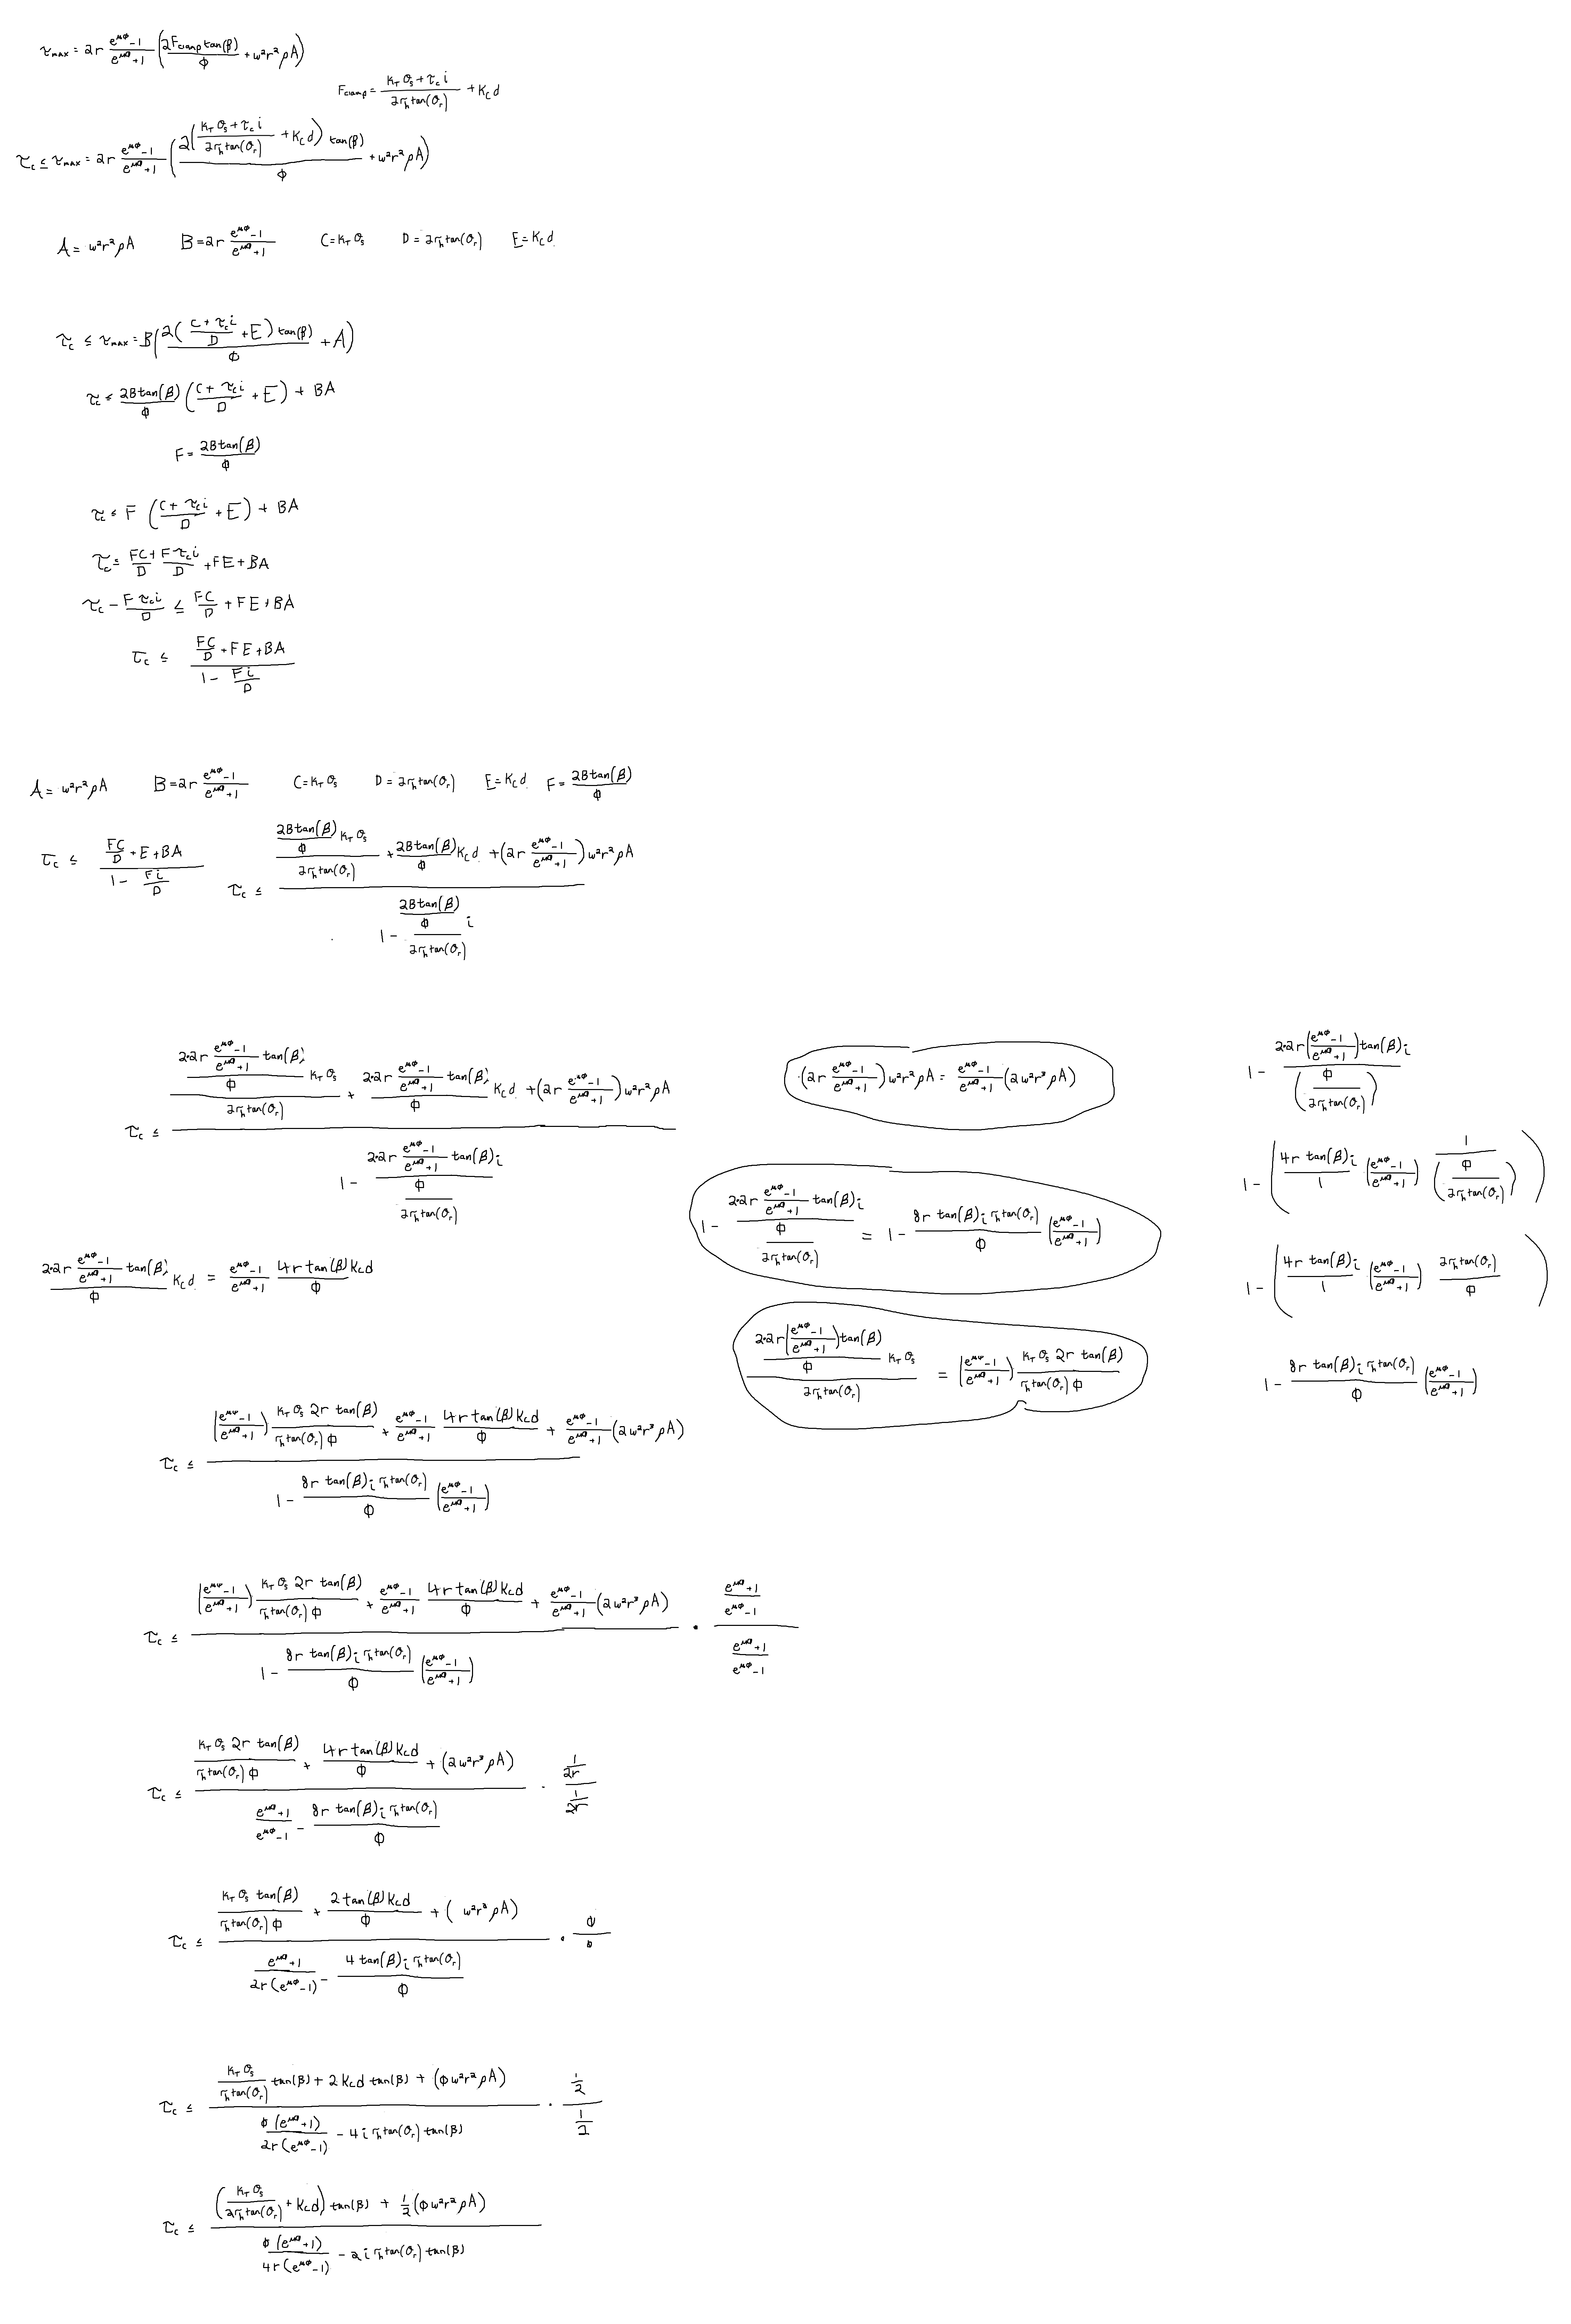
\includegraphics[width=0.75\linewidth]{../Kai's folder of derivations/t_maxSecondaryDerivation.png}
\label{fig:secondary_capacity_closure}
\end{figure}


\newpage
\bibliographystyle{plainnat}
\bibliography{../../refs/References}

\end{document}
